\chapter{Experimentos e Resultados}
\label{cap:resultados}

\section{Configuração Experimental}
\label{sec:configuracao_experimental}

Os experimentos realizados neste trabalho buscaram avaliar a eficácia da abordagem proposta, que combina curriculum learning e self-play para o treinamento de agentes no ambiente de futebol de robôs. Para garantir uma avaliação consistente e comparativa, foi estabelecida uma configuração experimental padronizada, detalhada nesta seção.

\subsection{Hardware Utilizado}

Todos os experimentos foram executados em um ambiente computacional de alto desempenho, com especificações adequadas para treinamento de aprendizado por reforço distribuído. A configuração de hardware incluiu:

\begin{itemize}
    \item Processador: AMD Ryzen 7 7700x com 16 núcleos virtuais
    \item Memória RAM: 32GB DDR5
    \item GPU: NVIDIA GeForce RTX 3090 com 24GB de memória VRAM
    \item Armazenamento: SSD NVMe de 2TB para leitura e escrita rápidas de checkpoints
\end{itemize}

A utilização de hardware especializado foi fundamental para viabilizar o treinamento distribuído com múltiplos trabalhadores paralelos, acelerando significativamente o processo experimental.

\subsection{Parâmetros de Treinamento}

Os parâmetros de treinamento foram cuidadosamente selecionados para garantir um equilíbrio entre eficiência computacional e qualidade do aprendizado, tentando mater o mais próximo possível do padrão utilizado no artigo original. Os principais parâmetros utilizados incluem:

\begin{itemize}
    \item \textbf{Algoritmo}: Proximal Policy Optimization (PPO) 
    \item \textbf{Taxa de aprendizado}: 0.0004 - Define o tamanho dos passos durante a otimização, controlando a velocidade do aprendizado
    \item \textbf{Função de ativação}: ReLU - Função não-linear que permite à rede neural aprender padrões complexos, zerando valores negativos
    \item \textbf{Arquitetura da rede neural}: Fully Connected com camadas [300, 200, 100] - Estrutura da rede neural com três camadas ocultas totalmente conectadas
    \item \textbf{Batch size}: 96000 (calculado como workers x envs x fragment) - Quantidade total de amostras processadas em cada iteração de treinamento
    \item \textbf{Mini-batch size}: 24000 (batch/4) - Subdivisão do batch para processamento em lotes menores, otimizando o uso de memória
    \item \textbf{Número de workers}: 12 (ambientes paralelos) - Quantidade de processos paralelos executando o ambiente de simulação
    \item \textbf{Ambientes por workers}: 4 - Número de ambientes simultâneos gerenciados por cada worker
    \item \textbf{Gamma}: 0.99 - Fator de desconto que determina a importância de recompensas futuras
    \item \textbf{Lambda}: 0.95 - Parâmetro de equilíbrio entre viés e variância no cálculo da vantagem generalizada
    \item \textbf{Coeficiente de entropia}: 0.01 - Incentiva a exploração ao adicionar aleatoriedade na política
    \item \textbf{Clip param}: 0.2 - Limita o tamanho das atualizações da política para evitar mudanças muito grandes
    \item \textbf{Iterações SGD}: 8 - Número de passos de otimização realizados em cada batch de dados
\end{itemize}

No caso específico do curriculum learning, foram configurados dois estágios progressivos, com parâmetros específicos para cada um, conforme detalhado no Capítulo 3. A taxa de promoção entre estágios foi estabelecida em 80\% de sucesso em uma janela de 100 episódios.

Para todos os experimentos realizados, foi definido um limite máximo de 900 iterações de treinamento, proporcionando uma base comparativa consistente entre as diferentes abordagens. No entanto, o número efetivo de iterações variou conforme o tipo de experimento e a complexidade das tarefas envolvidas, como pode ser observado na Tabela \ref{tab:iteracoes_experimentos}.

\begin{table}[h]
    \centering
    \caption{Número de iterações por experimento}
    \label{tab:iteracoes_experimentos}
    \begin{tabular}{|l|c|}
        \hline
        \textbf{Experimento} & \textbf{Total de Iterações} \\
        \hline
        Curriculum Task 0 & 55 \\
        Curriculum Task 1 & 60 \\
        Selfplay Após Curriculum & 781 \\
        Full Selfplay & 900 \\
        \hline
    \end{tabular}
\end{table}

Esta distribuição de iterações evidencia a diferença de complexidade entre as fases do treinamento, com as tarefas iniciais do curriculum exigindo significativamente menos iterações para convergência em comparação com as fases de self-play.

\subsection{Tempo de Treinamento}

O tempo total de treinamento para cada experimento foi medido em termos de horas de execução na configuração de hardware utilizada. A Figura \ref{fig:tempo_treinamento} apresenta uma comparação dos tempos de treinamento para as diferentes abordagens implementadas.

\begin{figure}[H]
    \centering
    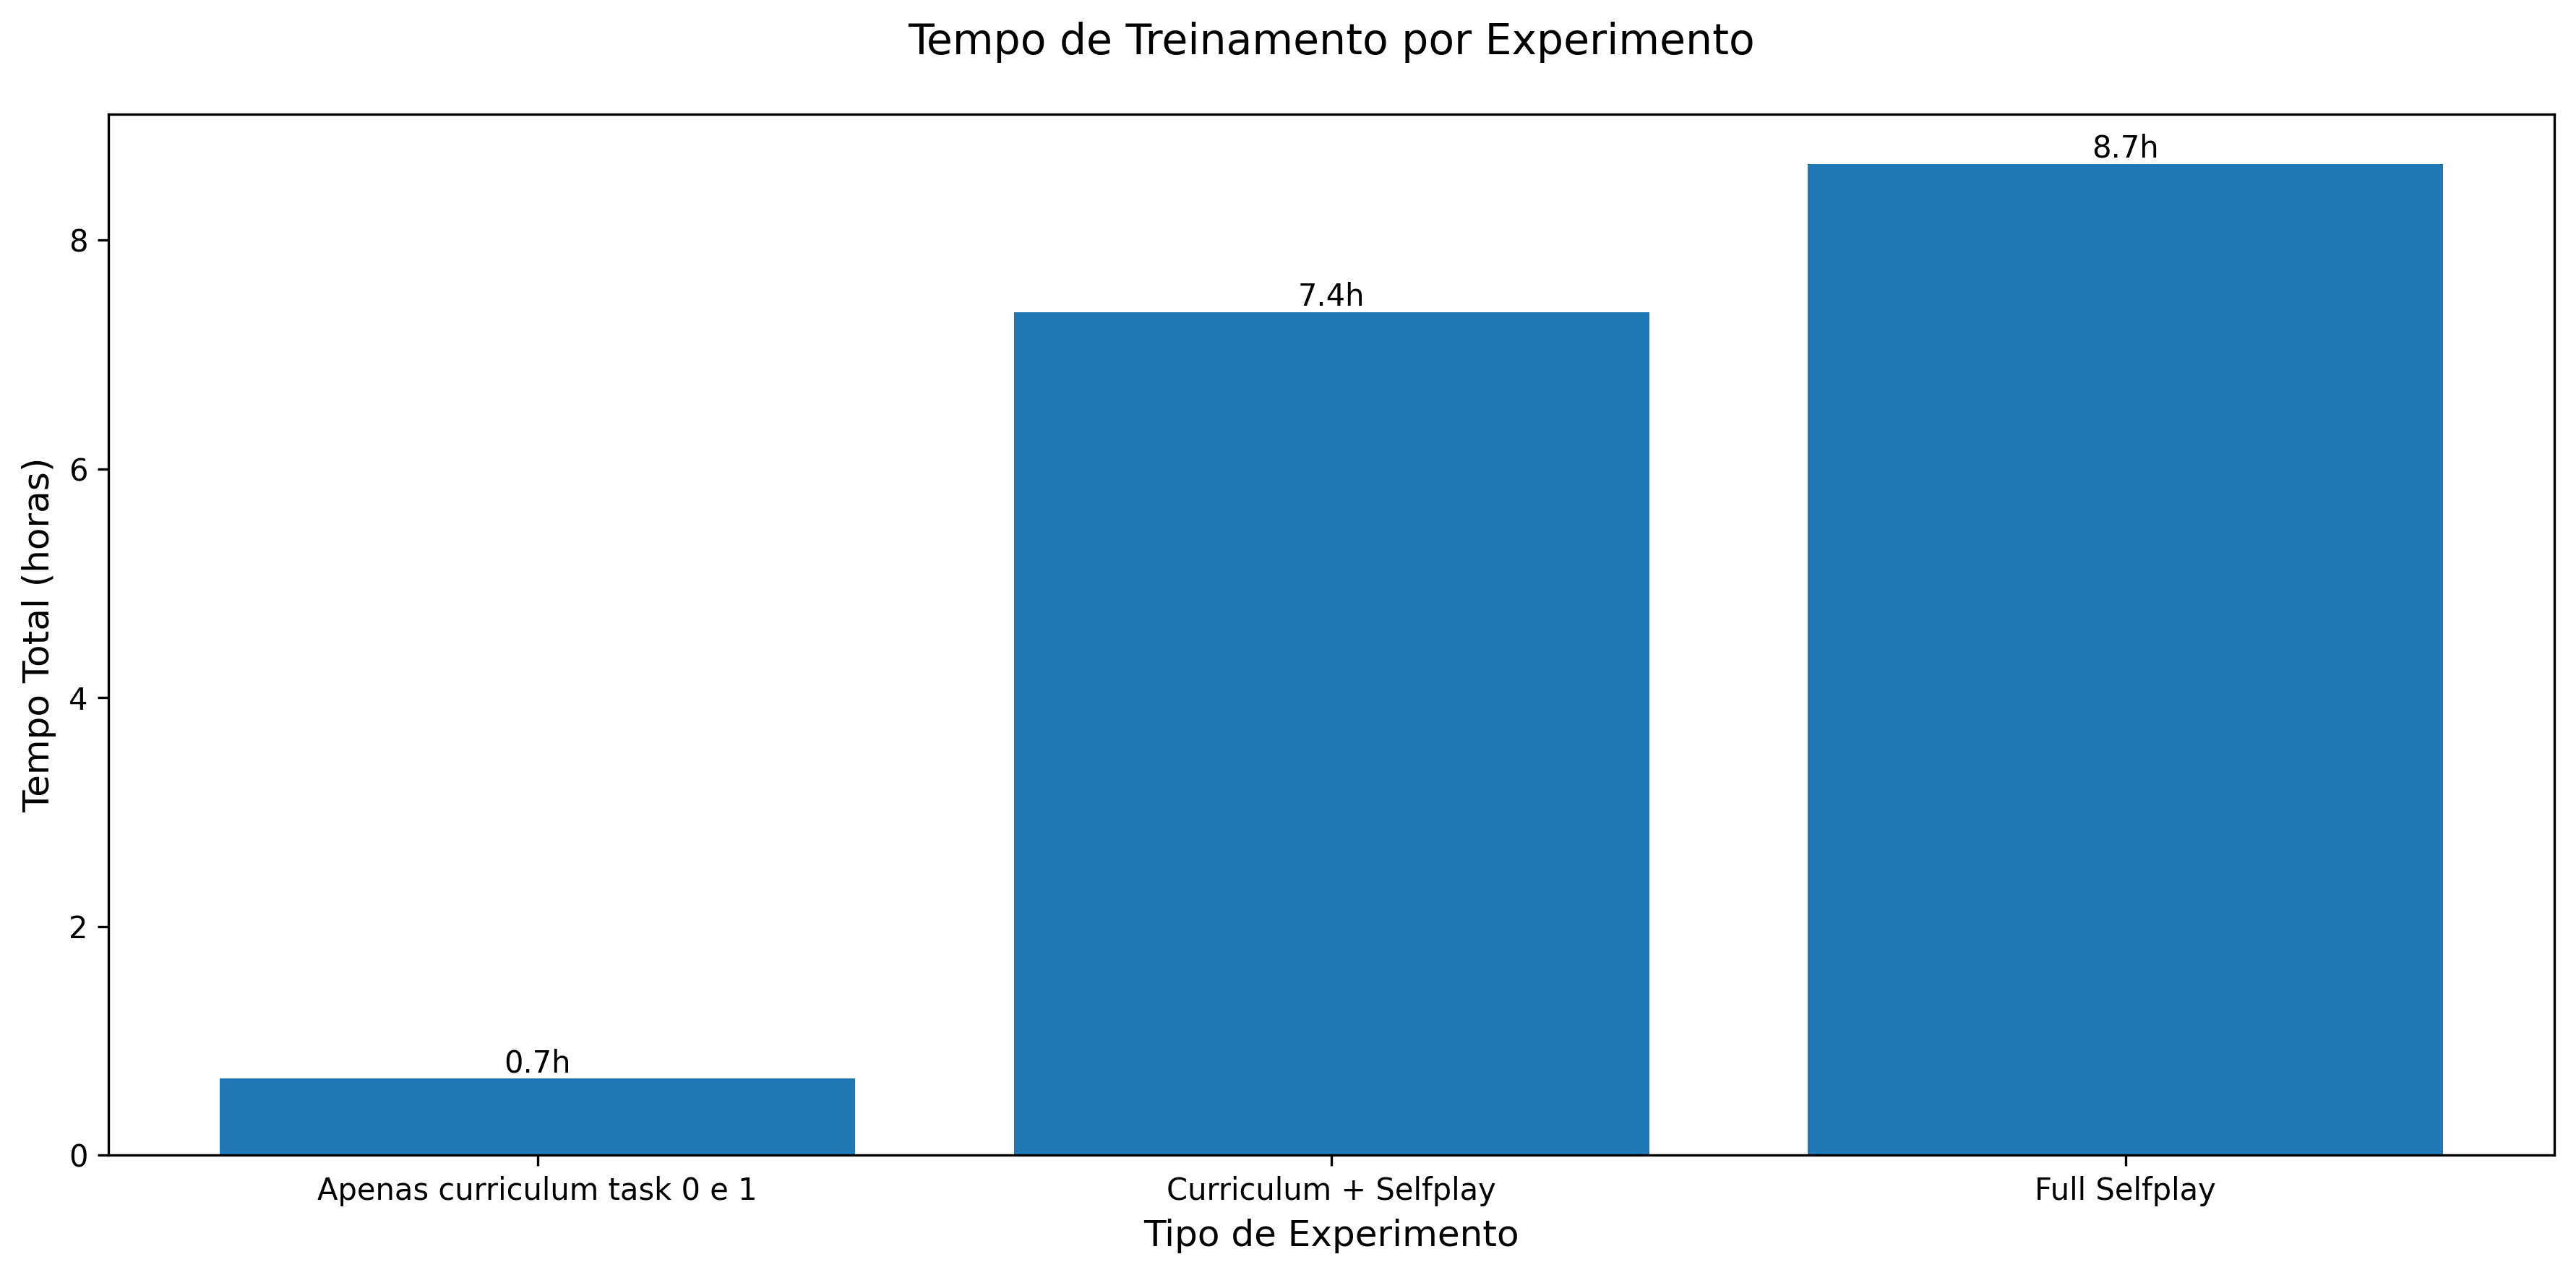
\includegraphics[width=0.9\textwidth]{fig/graficos_trabalho/graficos_experimentos/graficos_tempo_treino/tempo_treinamento.png}
    \caption{Comparação do tempo total de treinamento em horas para cada abordagem experimental}
    \label{fig:tempo_treinamento}
\end{figure}

A análise dos tempos de treinamento revela diferenças significativas entre as abordagens:

\begin{itemize}
    \item \textbf{Apenas curriculum (tasks 0 e 1)}: Aproximadamente 0,7 horas (42 minutos)
    \item \textbf{Curriculum + Self-play}: Aproximadamente 7,4 horas
    \item \textbf{Full Self-play}: Aproximadamente 8,7 horas
\end{itemize}

Estas diferenças nos tempos de treinamento refletem a complexidade e a natureza de cada abordagem. O treinamento exclusivo com curriculum tasks é significativamente mais rápido, pois envolve ambientes mais simples e objetivos bem definidos. A abordagem combinada (curriculum + self-play) apresenta um tempo de treinamento aproximadamente 15\% menor em relação ao full self-play tradicional.

Esta economia de tempo é uma observação particularmente relevante do ponto de vista prático, especialmente considerando que a abordagem combinada também proporcionou resultados superiores (conforme demonstrado nas seções anteriores). Esta vantagem em termos de eficiência computacional representa um aspecto importante para aplicações práticas, onde os recursos de processamento são frequentemente limitados.

A maior eficiência da abordagem combinada pode ser atribuída ao fato de que as habilidades fundamentais desenvolvidas durante o curriculum permitem que o agente aproveite melhor a fase de self-play, convergindo mais rapidamente para políticas efetivas. Os agentes que iniciam diretamente no self-play gastam mais tempo em fases iniciais de exploração aleatória, necessitando de iterações adicionais para desenvolver as mesmas capacidades que são adquiridas de forma estruturada no curriculum.

\section{Análise Comparativa}
\label{sec:analise_comparativa}

Para avaliar a eficácia da abordagem proposta, realizamos uma análise comparativa entre o modelo treinado apenas com self-play (baseline) e o modelo treinado com a combinação de curriculum learning e self-play (modelo proposto). Esta análise abrange diversas métricas relevantes para o domínio do futebol de robôs.

\subsection{Evolução da Recompensa}

A análise da evolução da recompensa média ao longo do treinamento oferece insights valiosos sobre o processo de aprendizagem dos agentes. A Figura \ref{fig:episode_reward} apresenta esta evolução para ambas as abordagens.

\begin{figure}[H]
    \centering
    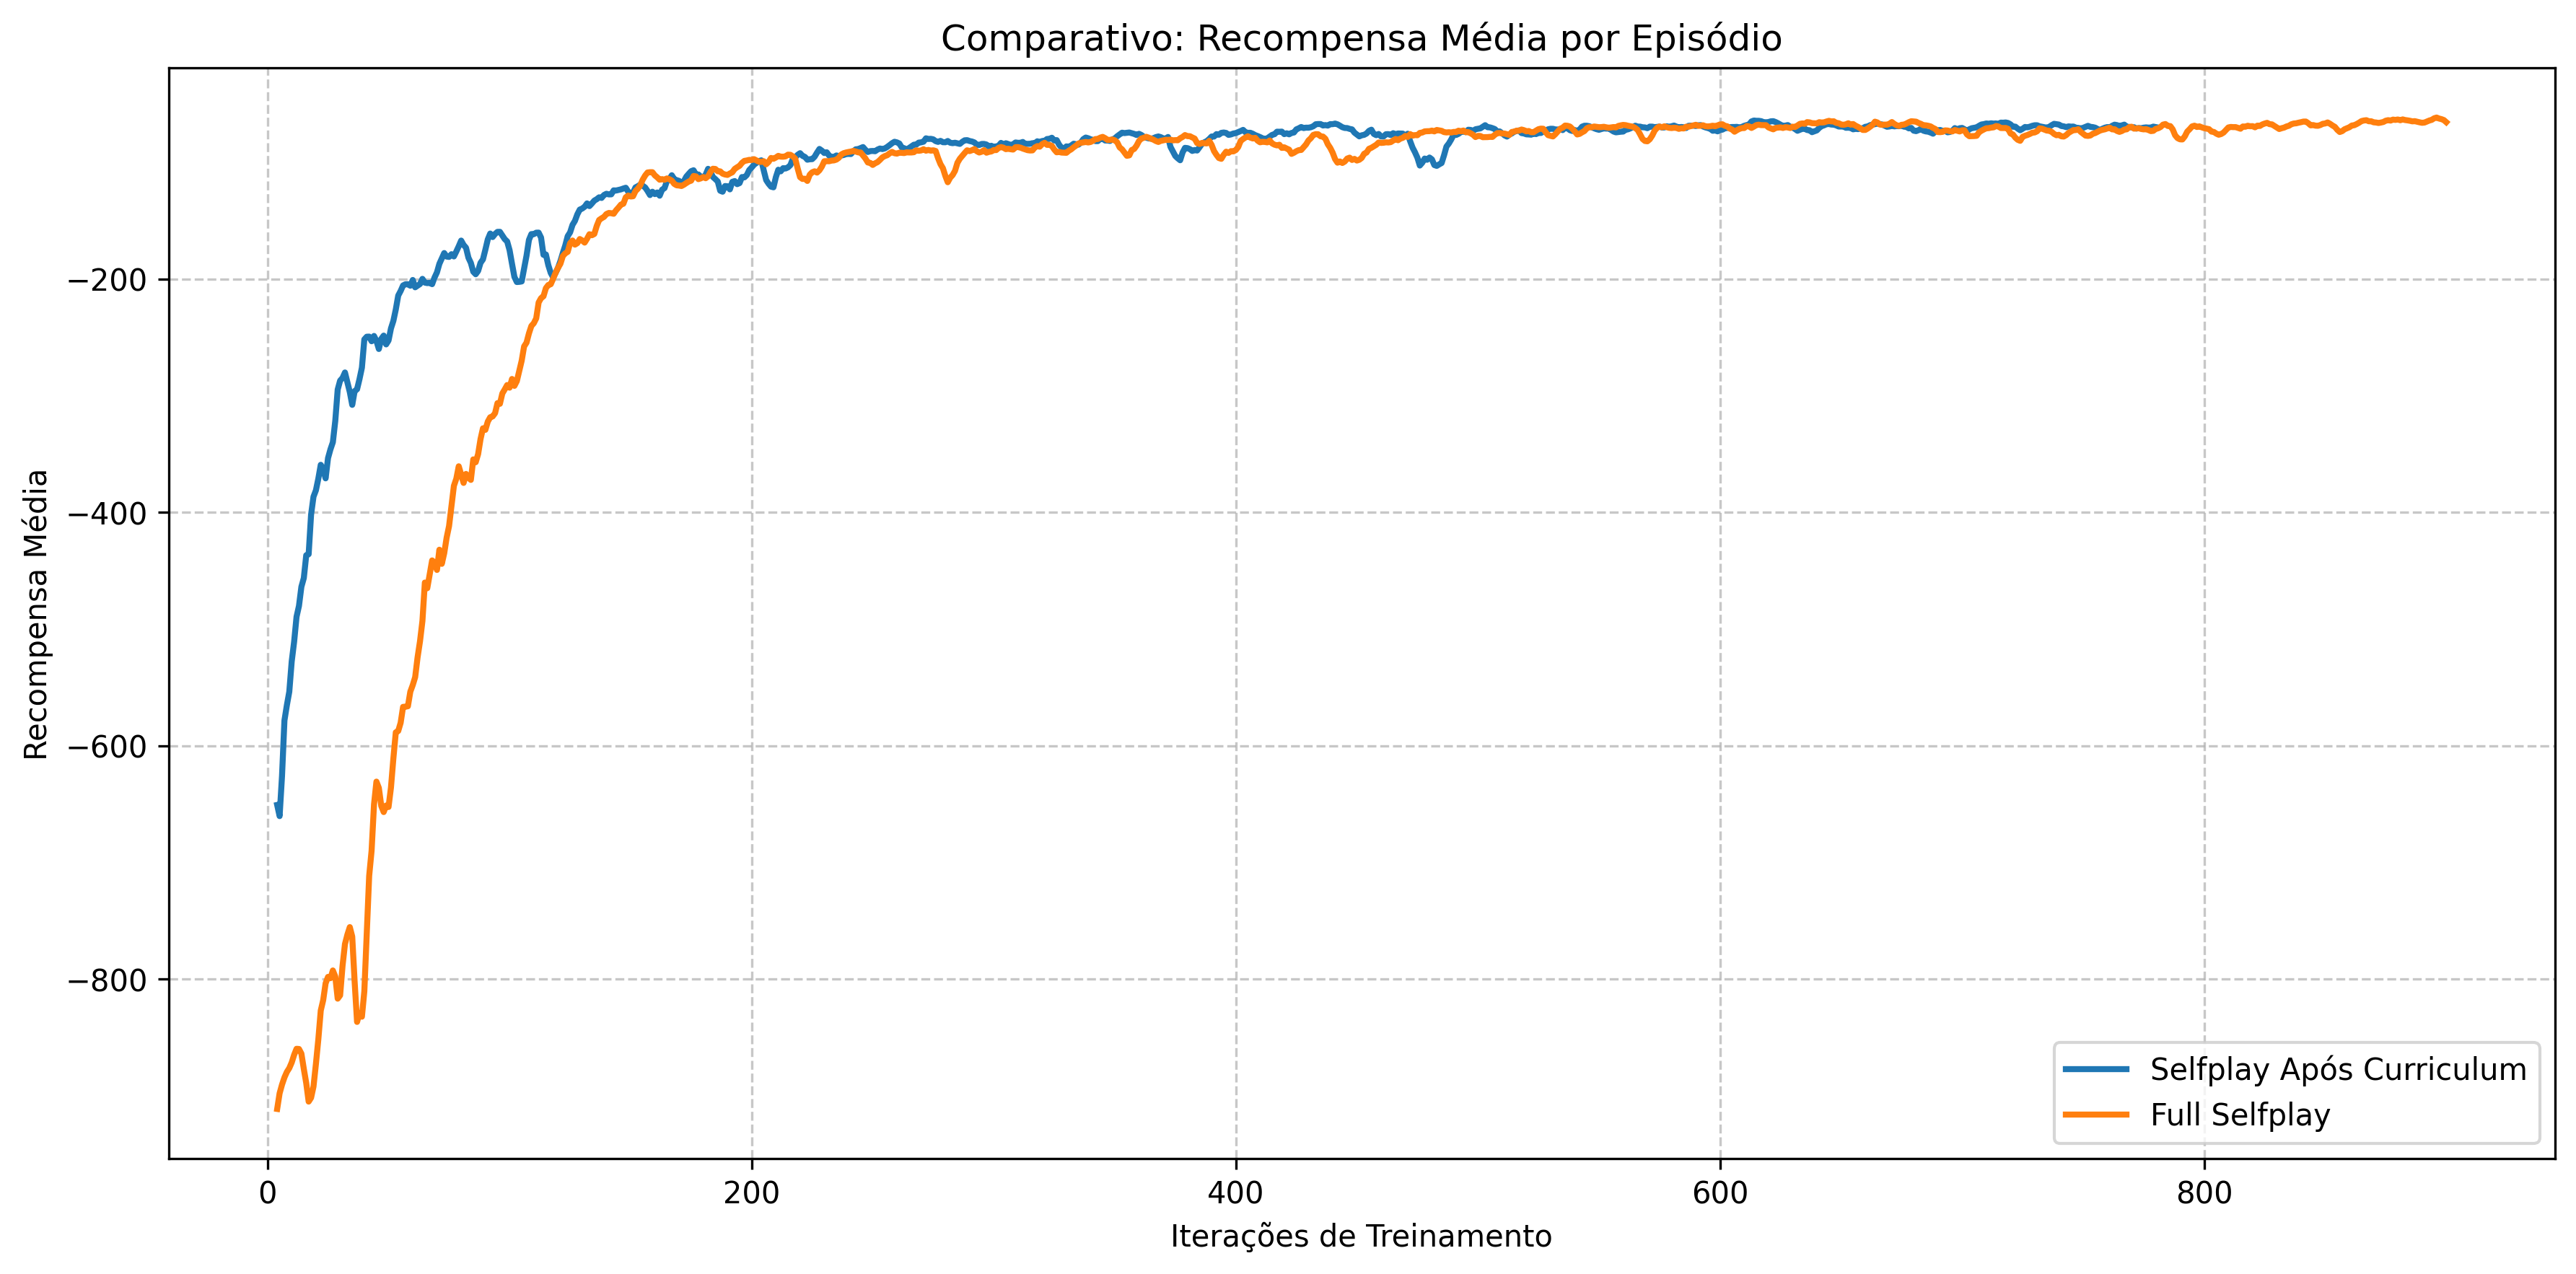
\includegraphics[width=0.8\textwidth]{fig/graficos_trabalho/graficos_experimentos/geral/comparativo_recompensa_media.png}
    \caption{Evolução da recompensa média por episódio ao longo do treinamento}
    \label{fig:episode_reward}
\end{figure}

O gráfico revela que o modelo treinado com curriculum learning apresenta um crescimento mais acelerado da recompensa nas fases iniciais do treinamento. Esta vantagem inicial é atribuída à aprendizagem estruturada de habilidades fundamentais durante os estágios do curriculum. Embora ambas as abordagens apresentem convergência em termos de recompensa acumulada, o modelo proposto atinge níveis equivalentes com menos timesteps de treinamento, sugerindo maior eficiência no processo de aprendizagem.

Nota-se também que o modelo proposto apresenta menor variabilidade na curva de recompensa, indicando maior estabilidade durante o processo de treinamento.

Para compreender melhor como as habilidades fundamentais são desenvolvidas durante o curriculum, é interessante analisar a evolução da recompensa em cada estágio específico. As Figuras \ref{fig:reward_task0} e \ref{fig:reward_task1} apresentam esta evolução para os estágios Task 0 e Task 1, respectivamente.

\begin{figure}[H]
    \centering
    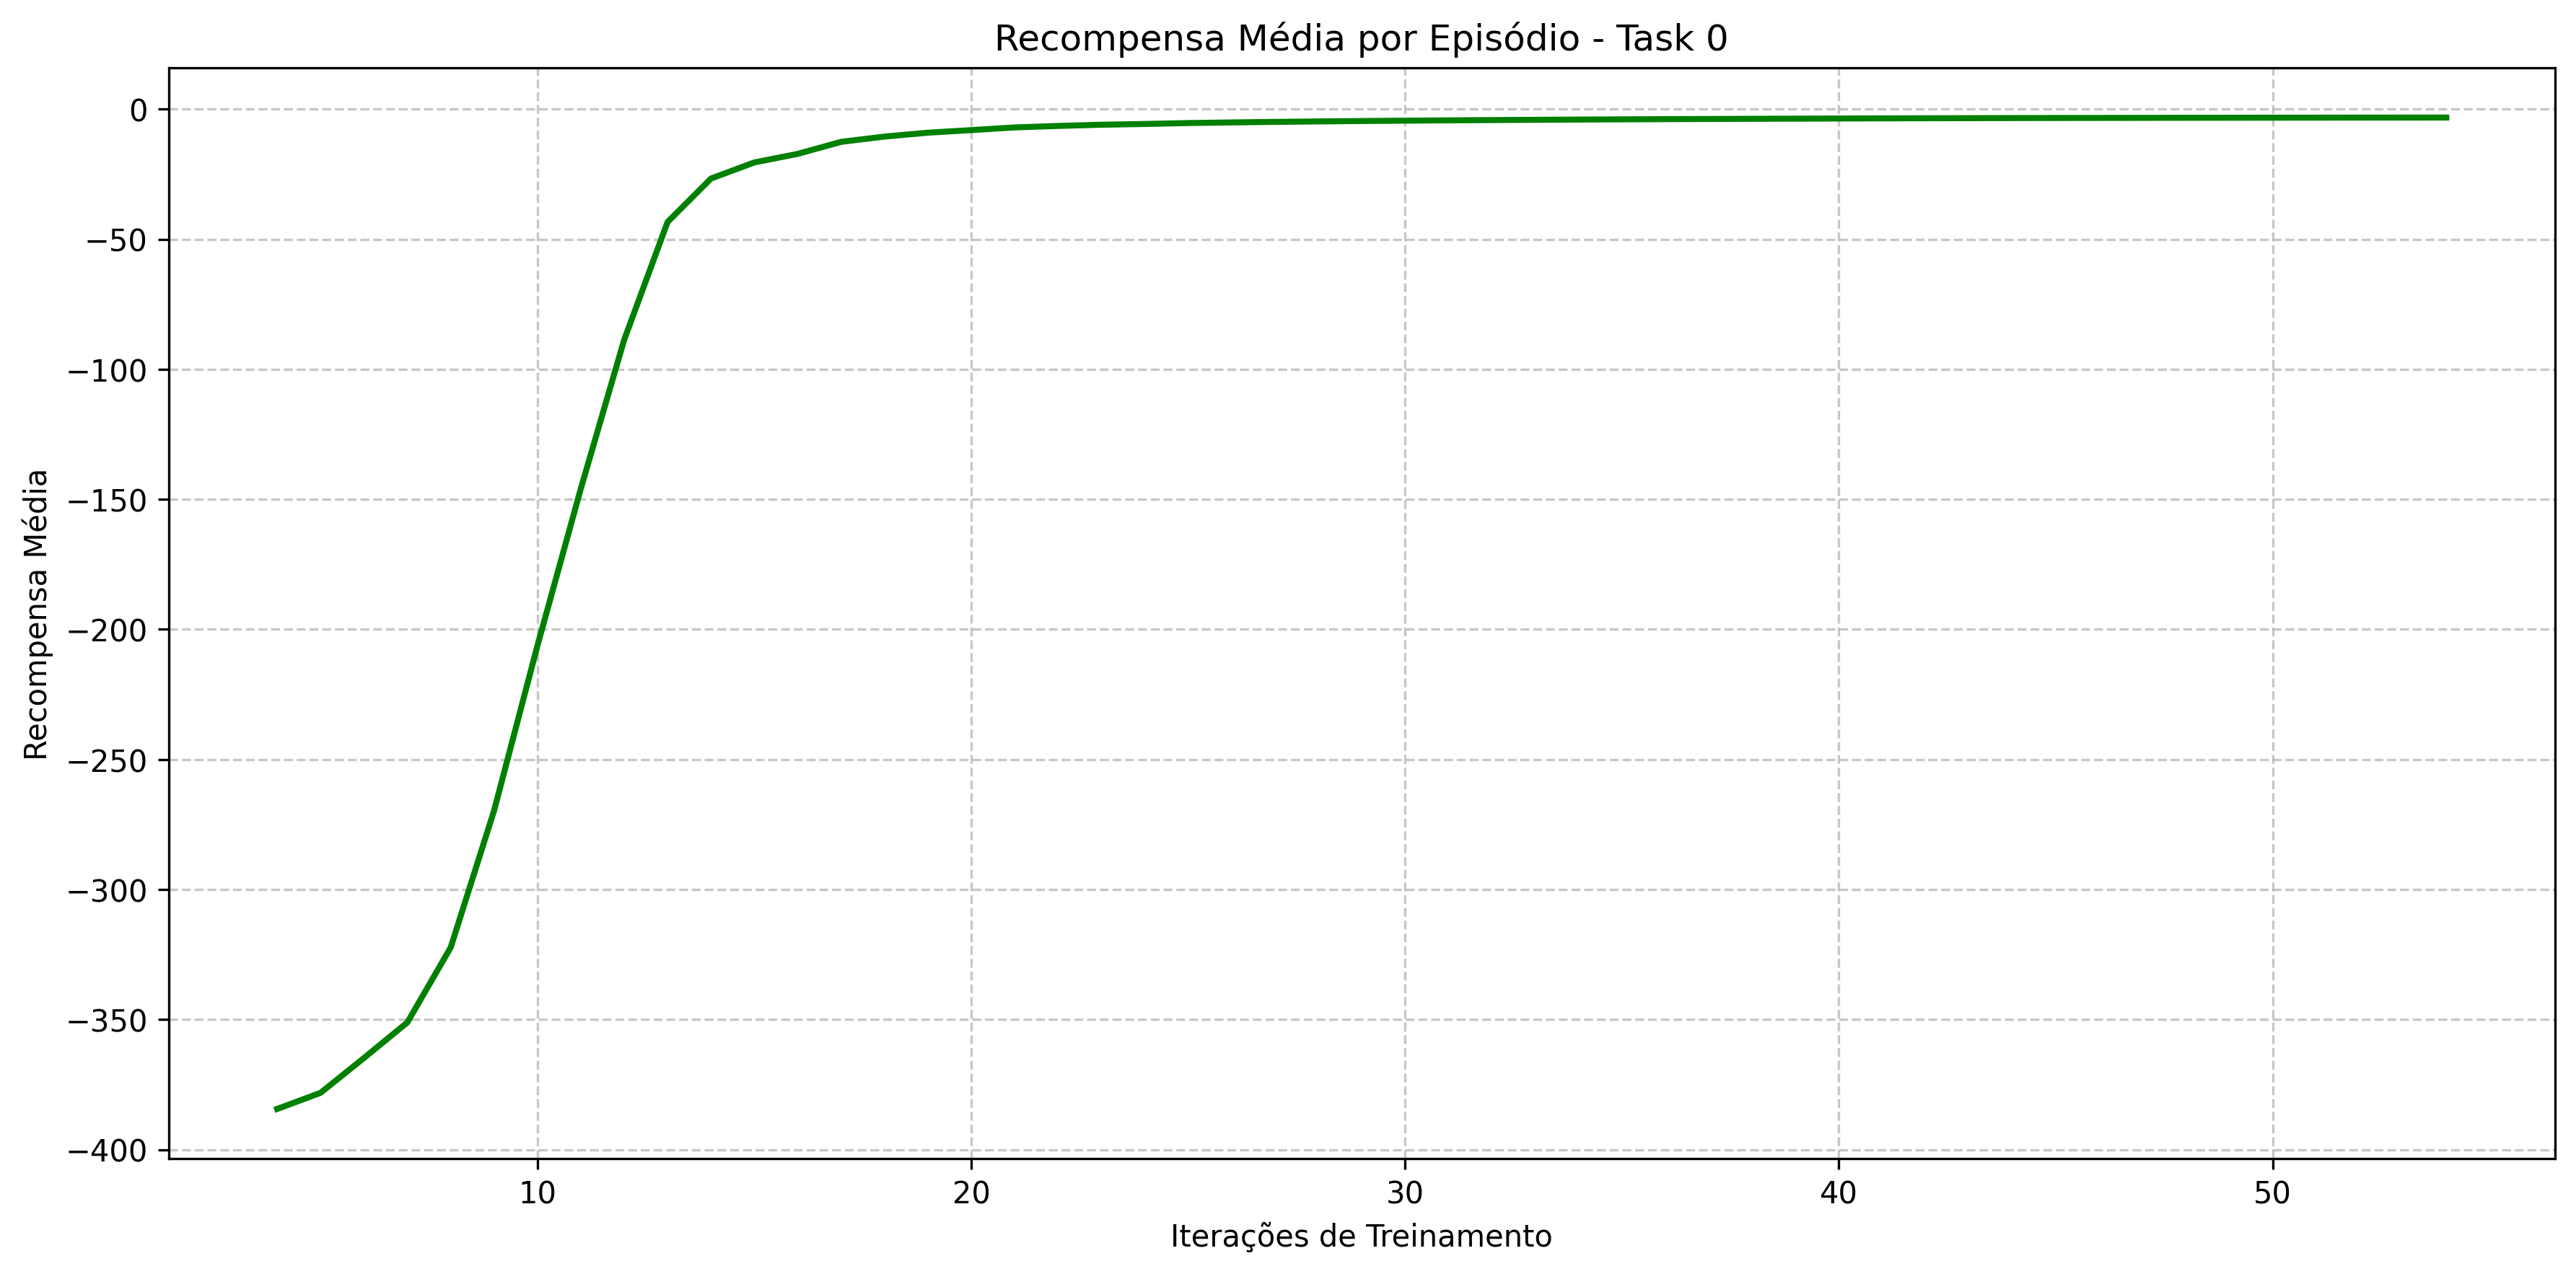
\includegraphics[width=0.8\textwidth]{fig/graficos_trabalho/graficos_experimentos/geral/recompensa_media_curriculum_task_0.png}
    \caption{Evolução da recompensa média por episódio durante o Curriculum Task 0}
    \label{fig:reward_task0}
\end{figure}

\begin{figure}[H]
    \centering
    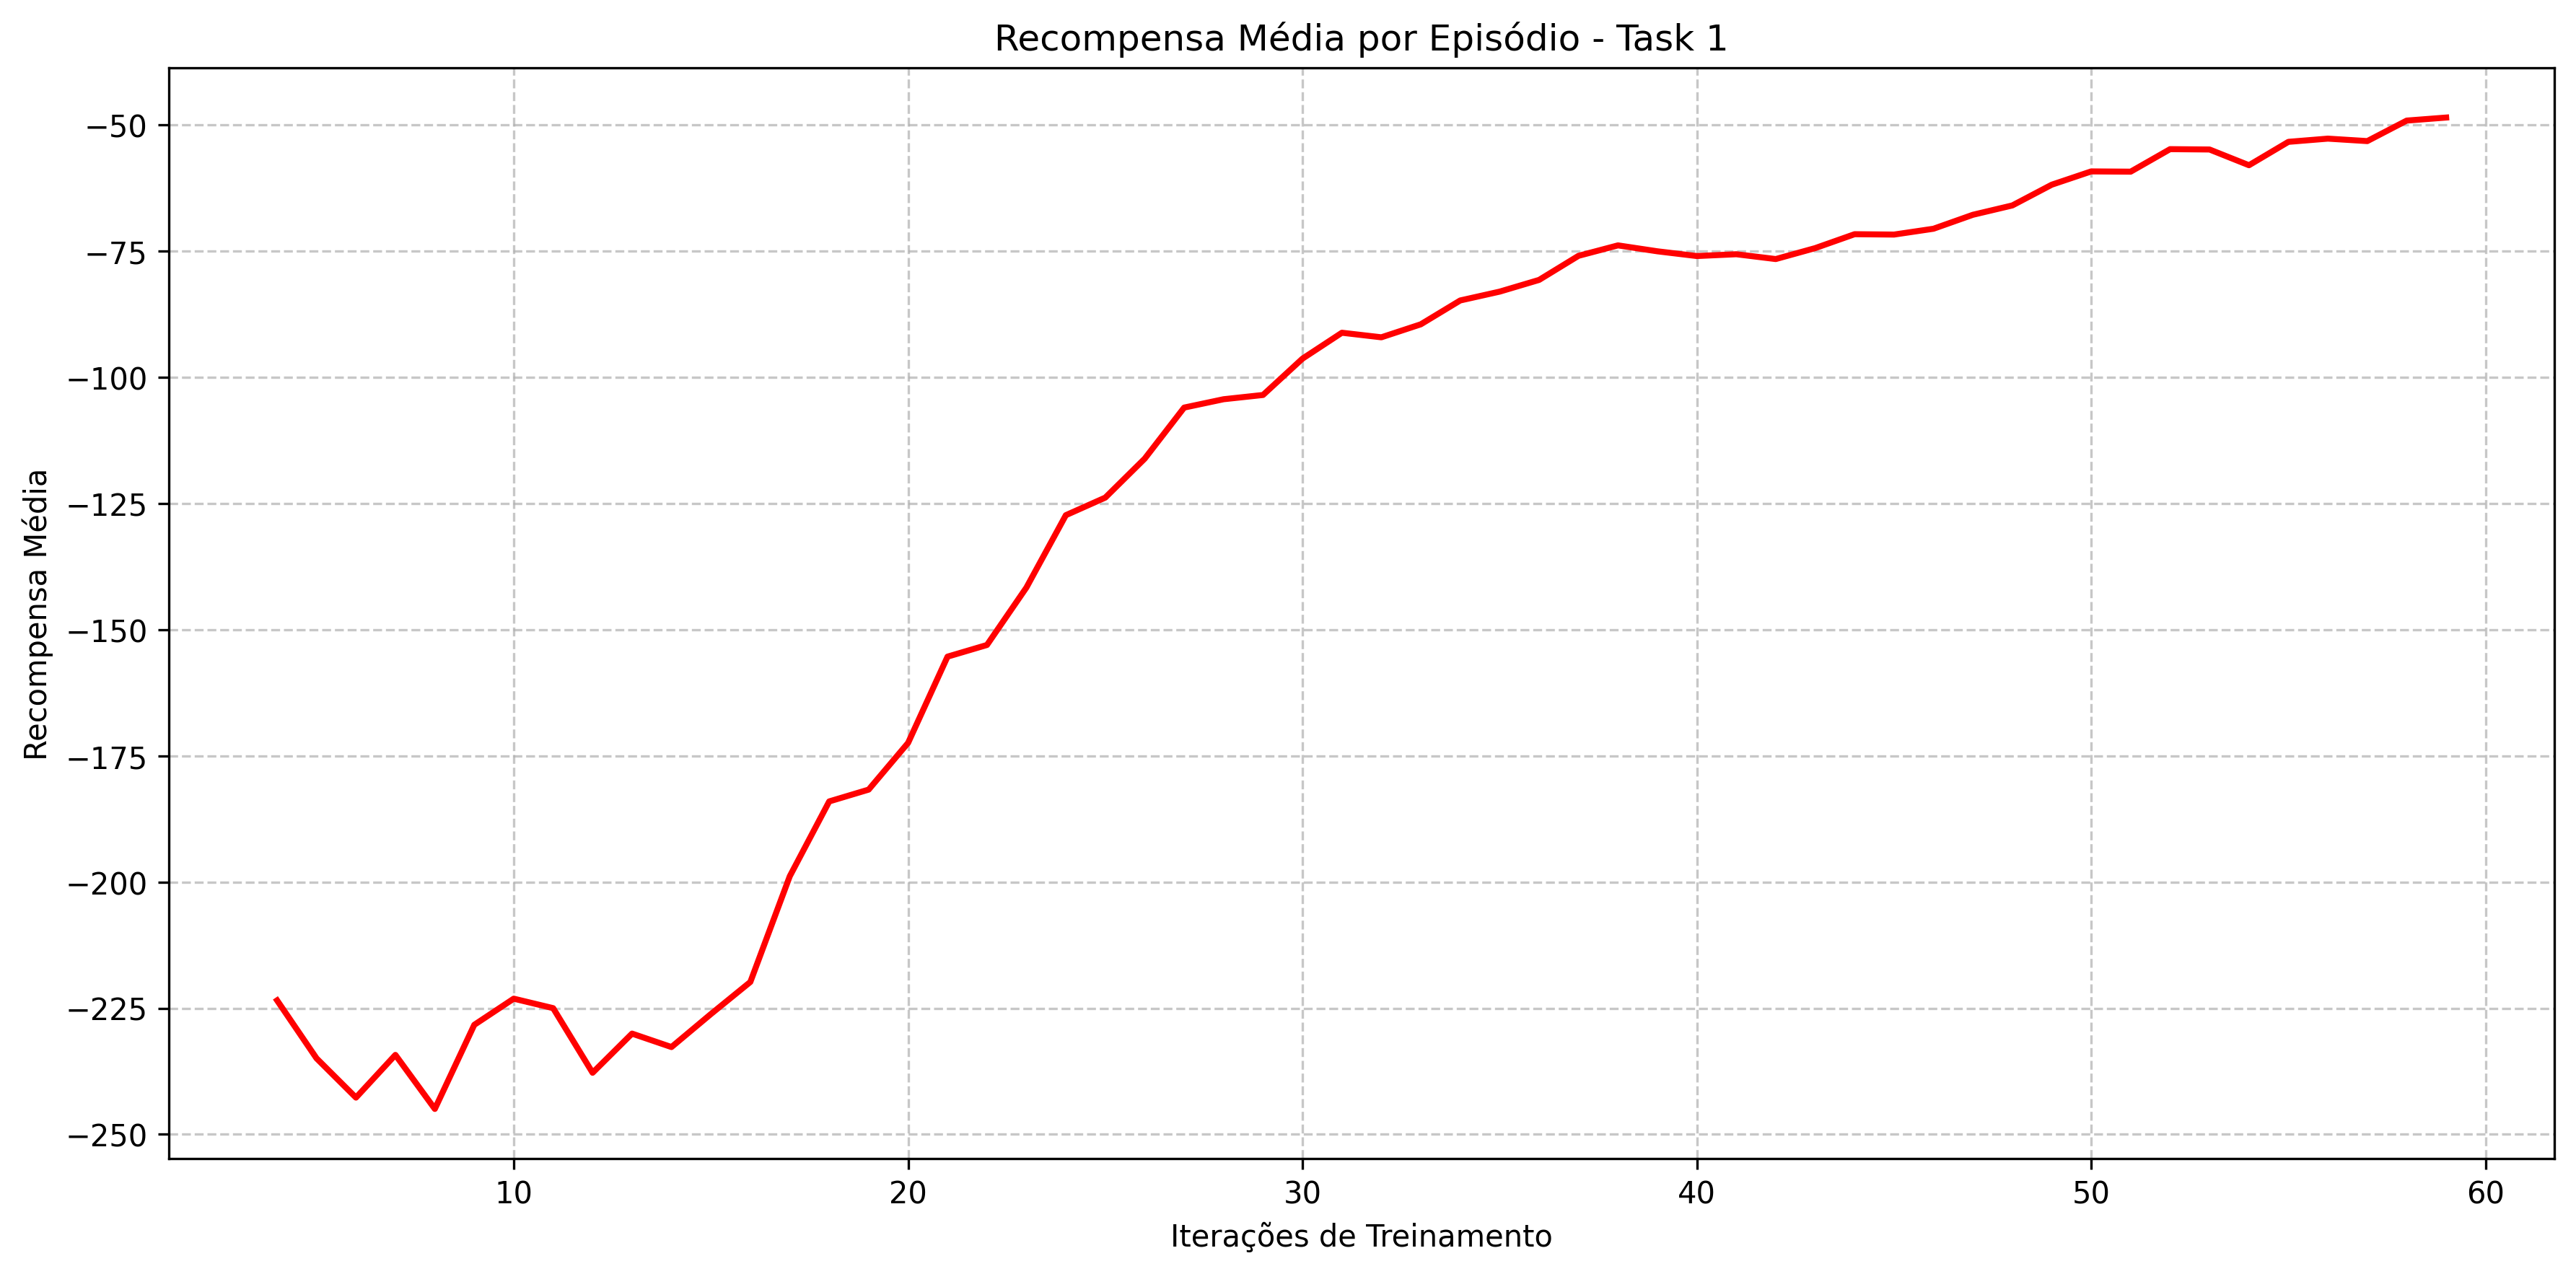
\includegraphics[width=0.8\textwidth]{fig/graficos_trabalho/graficos_experimentos/geral/recompensa_media_curriculum_task_1.png}
    \caption{Evolução da recompensa média por episódio durante o Curriculum Task 1}
    \label{fig:reward_task1}
\end{figure}

Estes gráficos revelam padrões distintos de aprendizado em cada estágio do curriculum. No Task 0 (Figura \ref{fig:reward_task0}), observa-se um crescimento acentuado da recompensa nas primeiras 15 iterações, partindo de valores próximos a -400 e estabilizando rapidamente em torno de 0. Esta evolução demonstra que os agentes aprendem eficientemente as habilidades básicas de controle e aproximação da bola, atingindo o critério de promoção em poucas iterações.

Já no Task 1 (Figura \ref{fig:reward_task1}), nota-se um padrão de aprendizado mais gradual e complexo. A curva apresenta oscilações iniciais entre as iterações 5 e 15, seguidas por um crescimento consistente até a iteração 60, quando a recompensa média atinge aproximadamente -50. Este comportamento reflete a maior complexidade desta tarefa, que exige coordenação entre múltiplos agentes e estratégias ofensivas mais sofisticadas na presença de oponentes estáticos.

A comparação entre estes dois estágios ilustra claramente a progressão de complexidade no curriculum e como os agentes desenvolvem diferentes habilidades em cada fase. O rápido progresso no Task 0 estabelece a base motora fundamental, enquanto o aprendizado mais gradual no Task 1 desenvolve capacidades táticas e coordenativas que serão cruciais durante o posterior treinamento com self-play.

\subsection{Desempenho Ofensivo}

O desempenho ofensivo dos agentes foi avaliado principalmente através da análise da taxa de sucesso na conclusão dos objetivos. A Figura \ref{fig:goals_blue_comparison} apresenta a evolução desta métrica ao longo do treinamento para ambas as abordagens.

\begin{figure}[H]
    \centering
    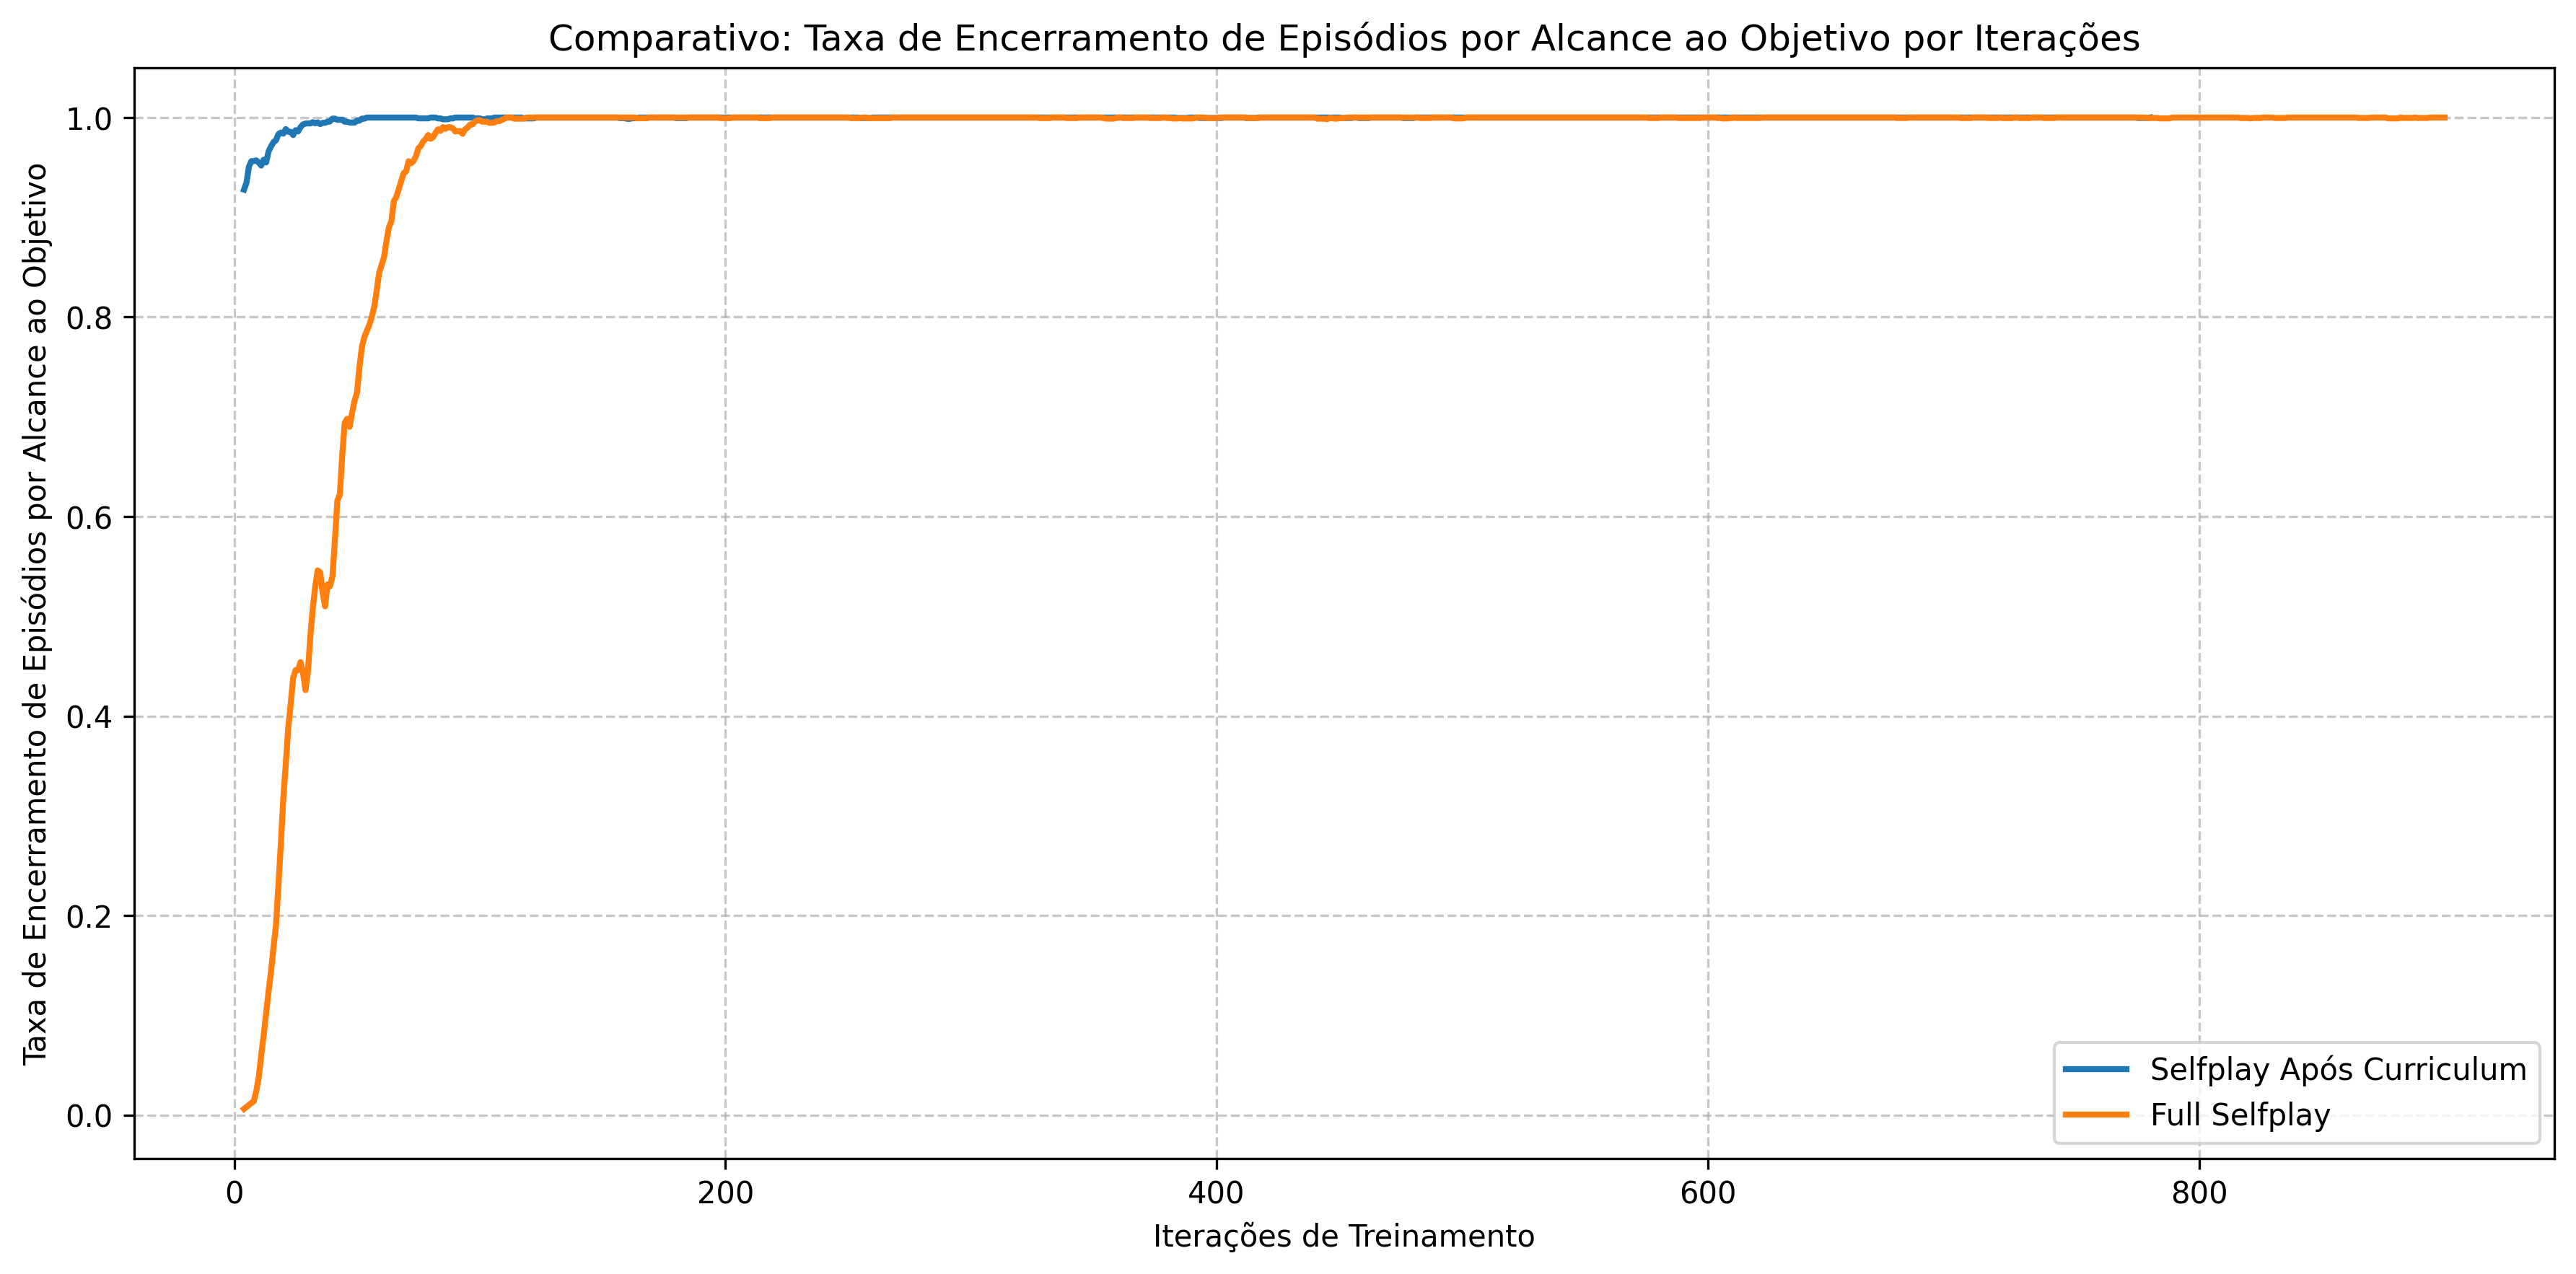
\includegraphics[width=0.95\textwidth]{fig/graficos_trabalho/graficos_experimentos/geral/comparativo_taxa_encerramento_episodios.png}
    \caption{Comparativo: Taxa de Encerramento de Episódios por Alcance ao Objetivo por Iterações entre as abordagens Selfplay após Curriculum e Full Selfplay}
    \label{fig:goals_blue_comparison}
\end{figure}

A análise comparativa do gráfico revela padrões interessantes na evolução da capacidade dos agentes de atingir seus objetivos. Ambas as abordagens apresentam uma progressão crescente na taxa de sucesso, eventualmente atingindo valores próximos a 100\%. No entanto, observam-se diferenças significativas no processo de aprendizado:

\begin{itemize}
    \item \textbf{Velocidade de convergência}: O Selfplay após Curriculum (linha azul) atinge o patamar próximo a 100\% de sucesso muito mais rapidamente, convergindo nas primeiras 50 iterações, enquanto o Full Selfplay (linha laranja) requer cerca de 150 iterações para alcançar desempenho semelhante.
    
    \item \textbf{Fase inicial}: Nas primeiras iterações, o Selfplay após Curriculum já começa com uma taxa de sucesso em torno de 90\%, demonstrando que as habilidades adquiridas durante a fase de curriculum proporcionam um ponto de partida significativamente mais avançado.
    
    \item \textbf{Estabilidade}: Ambas as abordagens eventualmente atingem estabilidade, mas o Selfplay após Curriculum apresenta menor variabilidade durante todo o processo, indicando um aprendizado mais consistente e robusto.
\end{itemize}

Esta comparação com iterações alinhadas evidencia de forma clara uma vantagem significativa da abordagem proposta: ao iniciar o self-play com agentes já treinados em tarefas fundamentais através do curriculum, obtém-se uma aceleração substancial na capacidade de atingir objetivos. Esta característica é particularmente valiosa em cenários com restrições de tempo computacional, onde a convergência mais rápida para políticas de alta qualidade representa uma vantagem considerável.

\subsection{Eficiência e Continuidade do Jogo}

Um aspecto diferencial da abordagem proposta é a melhoria significativa nas métricas relacionadas à continuidade do jogo, que refletem a capacidade dos agentes de manter a bola em jogo por períodos mais longos. A Figura \ref{fig:total_resets} apresenta a evolução do número médio de resets por episódio.

\begin{figure}[H]
    \centering
    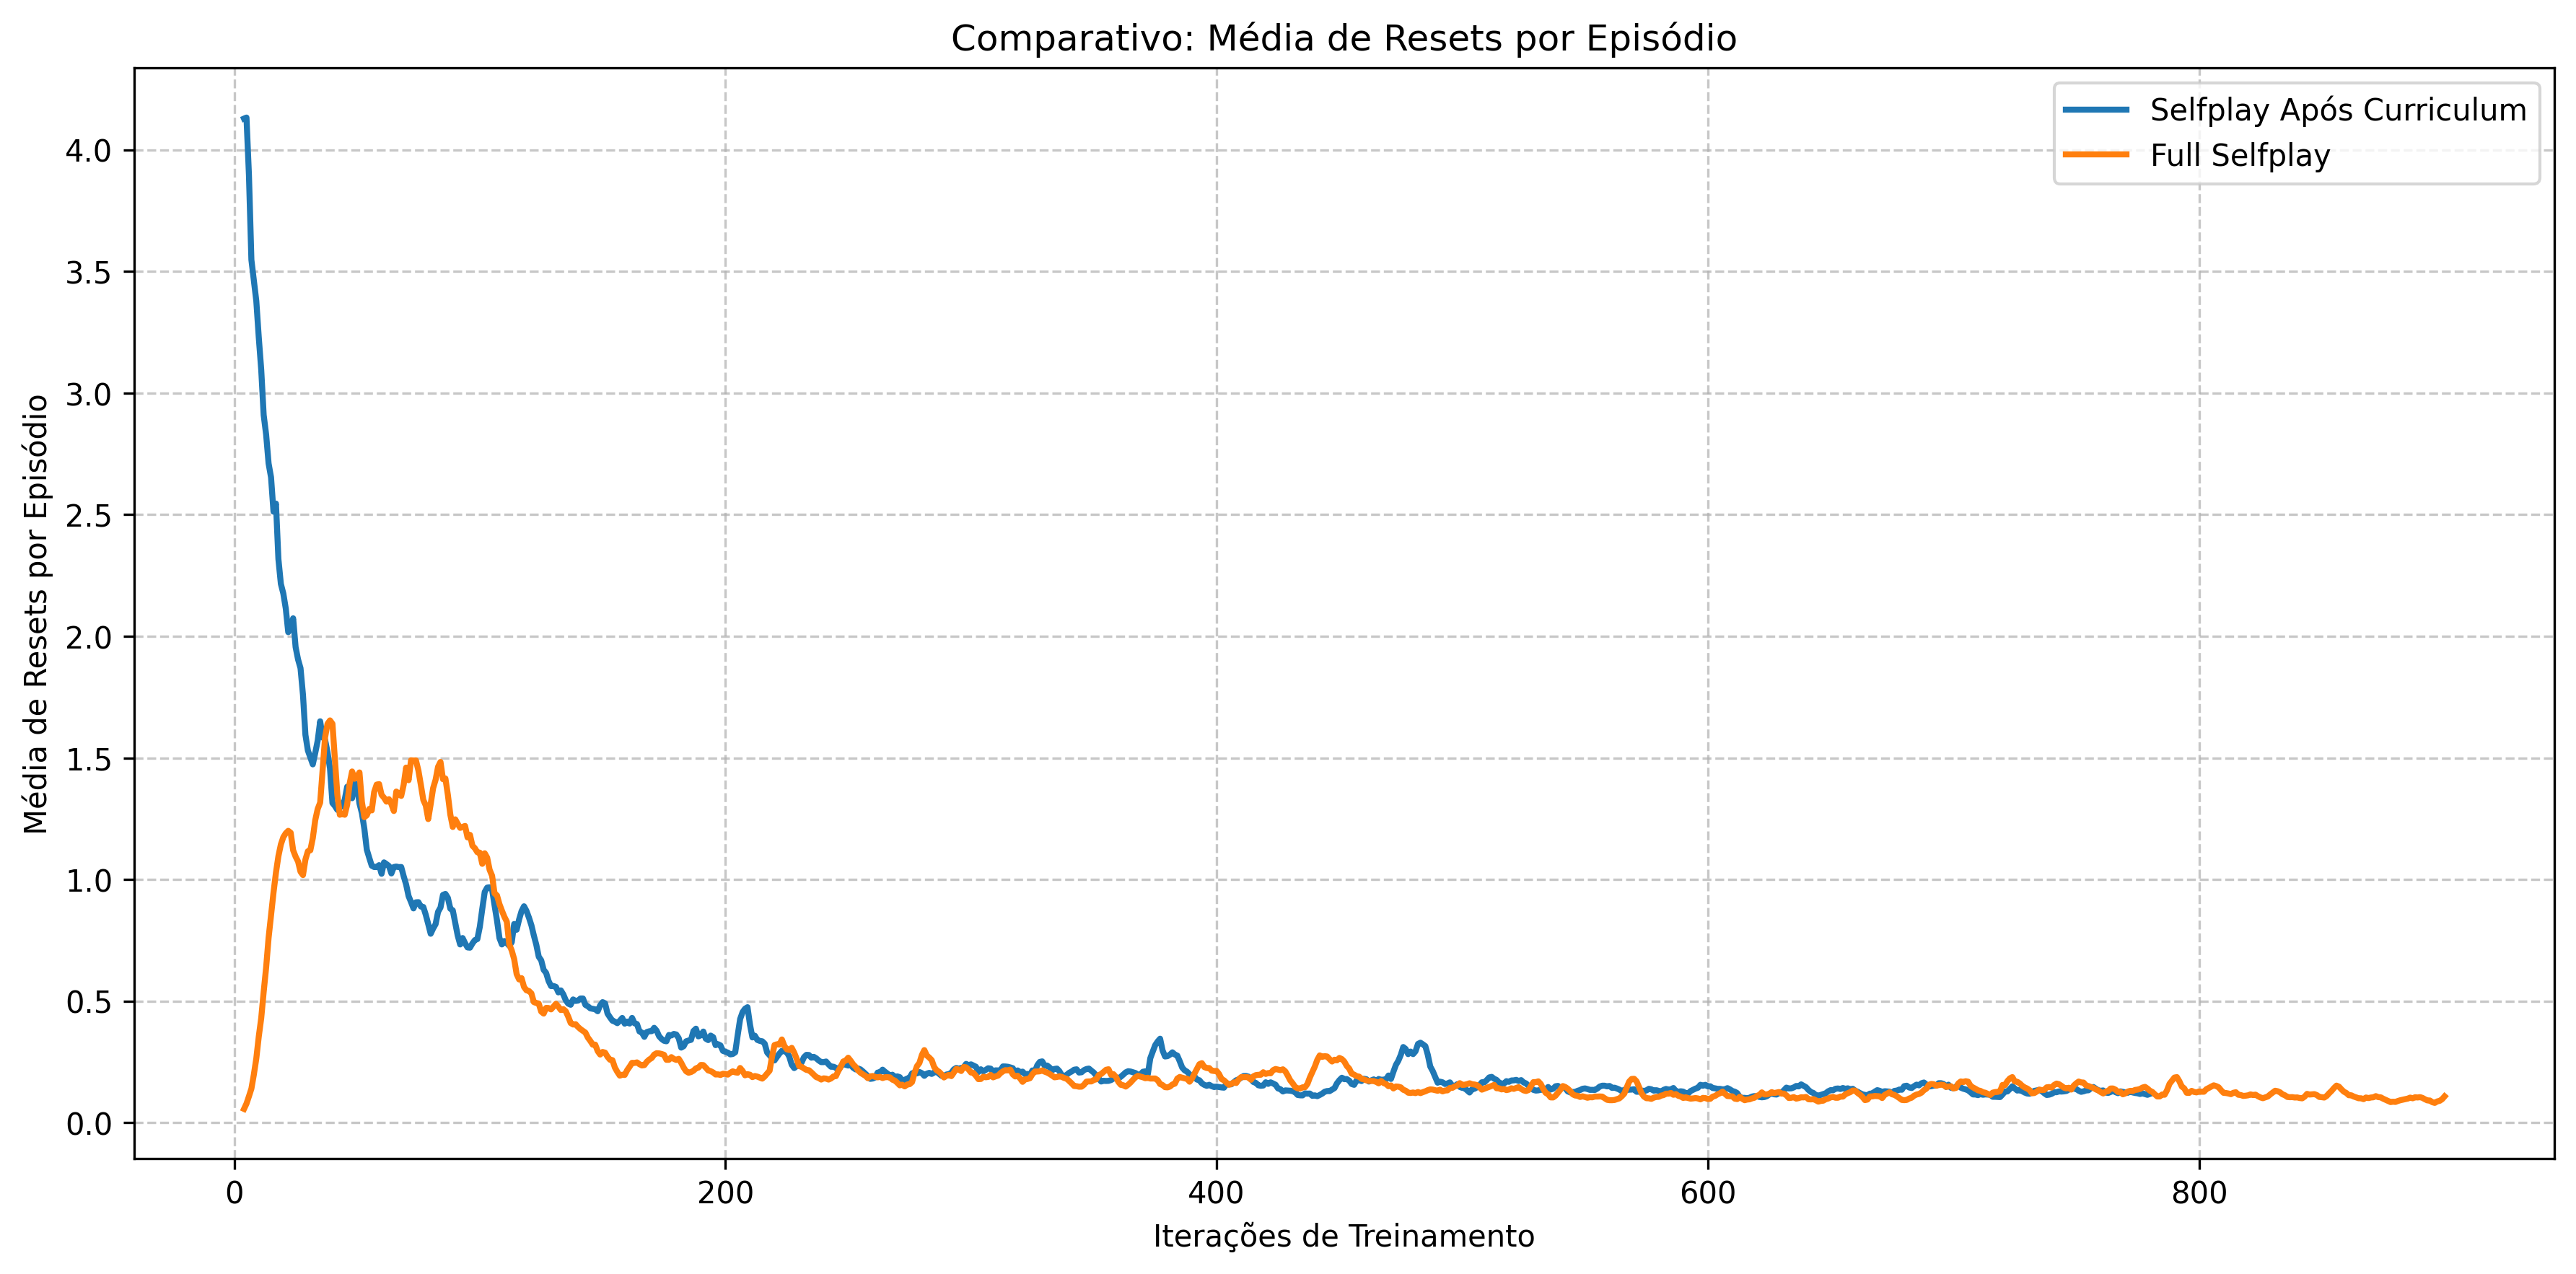
\includegraphics[width=0.95\textwidth]{fig/graficos_trabalho/graficos_experimentos/geral/comparativo_resets_por_episodio.png}
    \caption{Comparativo da média de resets por episódio com iterações alinhadas entre as abordagens Selfplay após Curriculum e Full Selfplay}
    \label{fig:total_resets}
\end{figure}

A análise do gráfico revela diferenças significativas nos padrões de aprendizado relacionados à continuidade do jogo. Inicialmente, o Selfplay após Curriculum (linha azul) apresenta um pico maior de resets por episódio, mas rapidamente consegue reduzir esse número. O Full Selfplay (linha laranja) mostra um comportamento diferente, com um aumento gradual seguido por uma redução mais lenta.

Após aproximadamente 200 iterações, ambas as abordagens convergem para valores similares, com ligeira vantagem para o Full Selfplay nas iterações finais. No entanto, é notável que o Selfplay após Curriculum consegue reduzir o número de resets de forma mais rápida nas fases iniciais do treinamento, evidenciando a transferência positiva das habilidades adquiridas durante o curriculum.

Complementarmente, a análise do tempo médio entre resets (Figura \ref{fig:time_between_resets}), que compara o intervalo de tempo entre as interrupções do jogo nas duas abordagens, reforça esta observação sobre os diferentes padrões de aprendizado. O gráfico apresenta o tempo médio entre resets ao longo das iterações de treinamento, permitindo avaliar a capacidade dos agentes em manter a bola em jogo por períodos mais longos.

\begin{figure}[H]
    \centering
    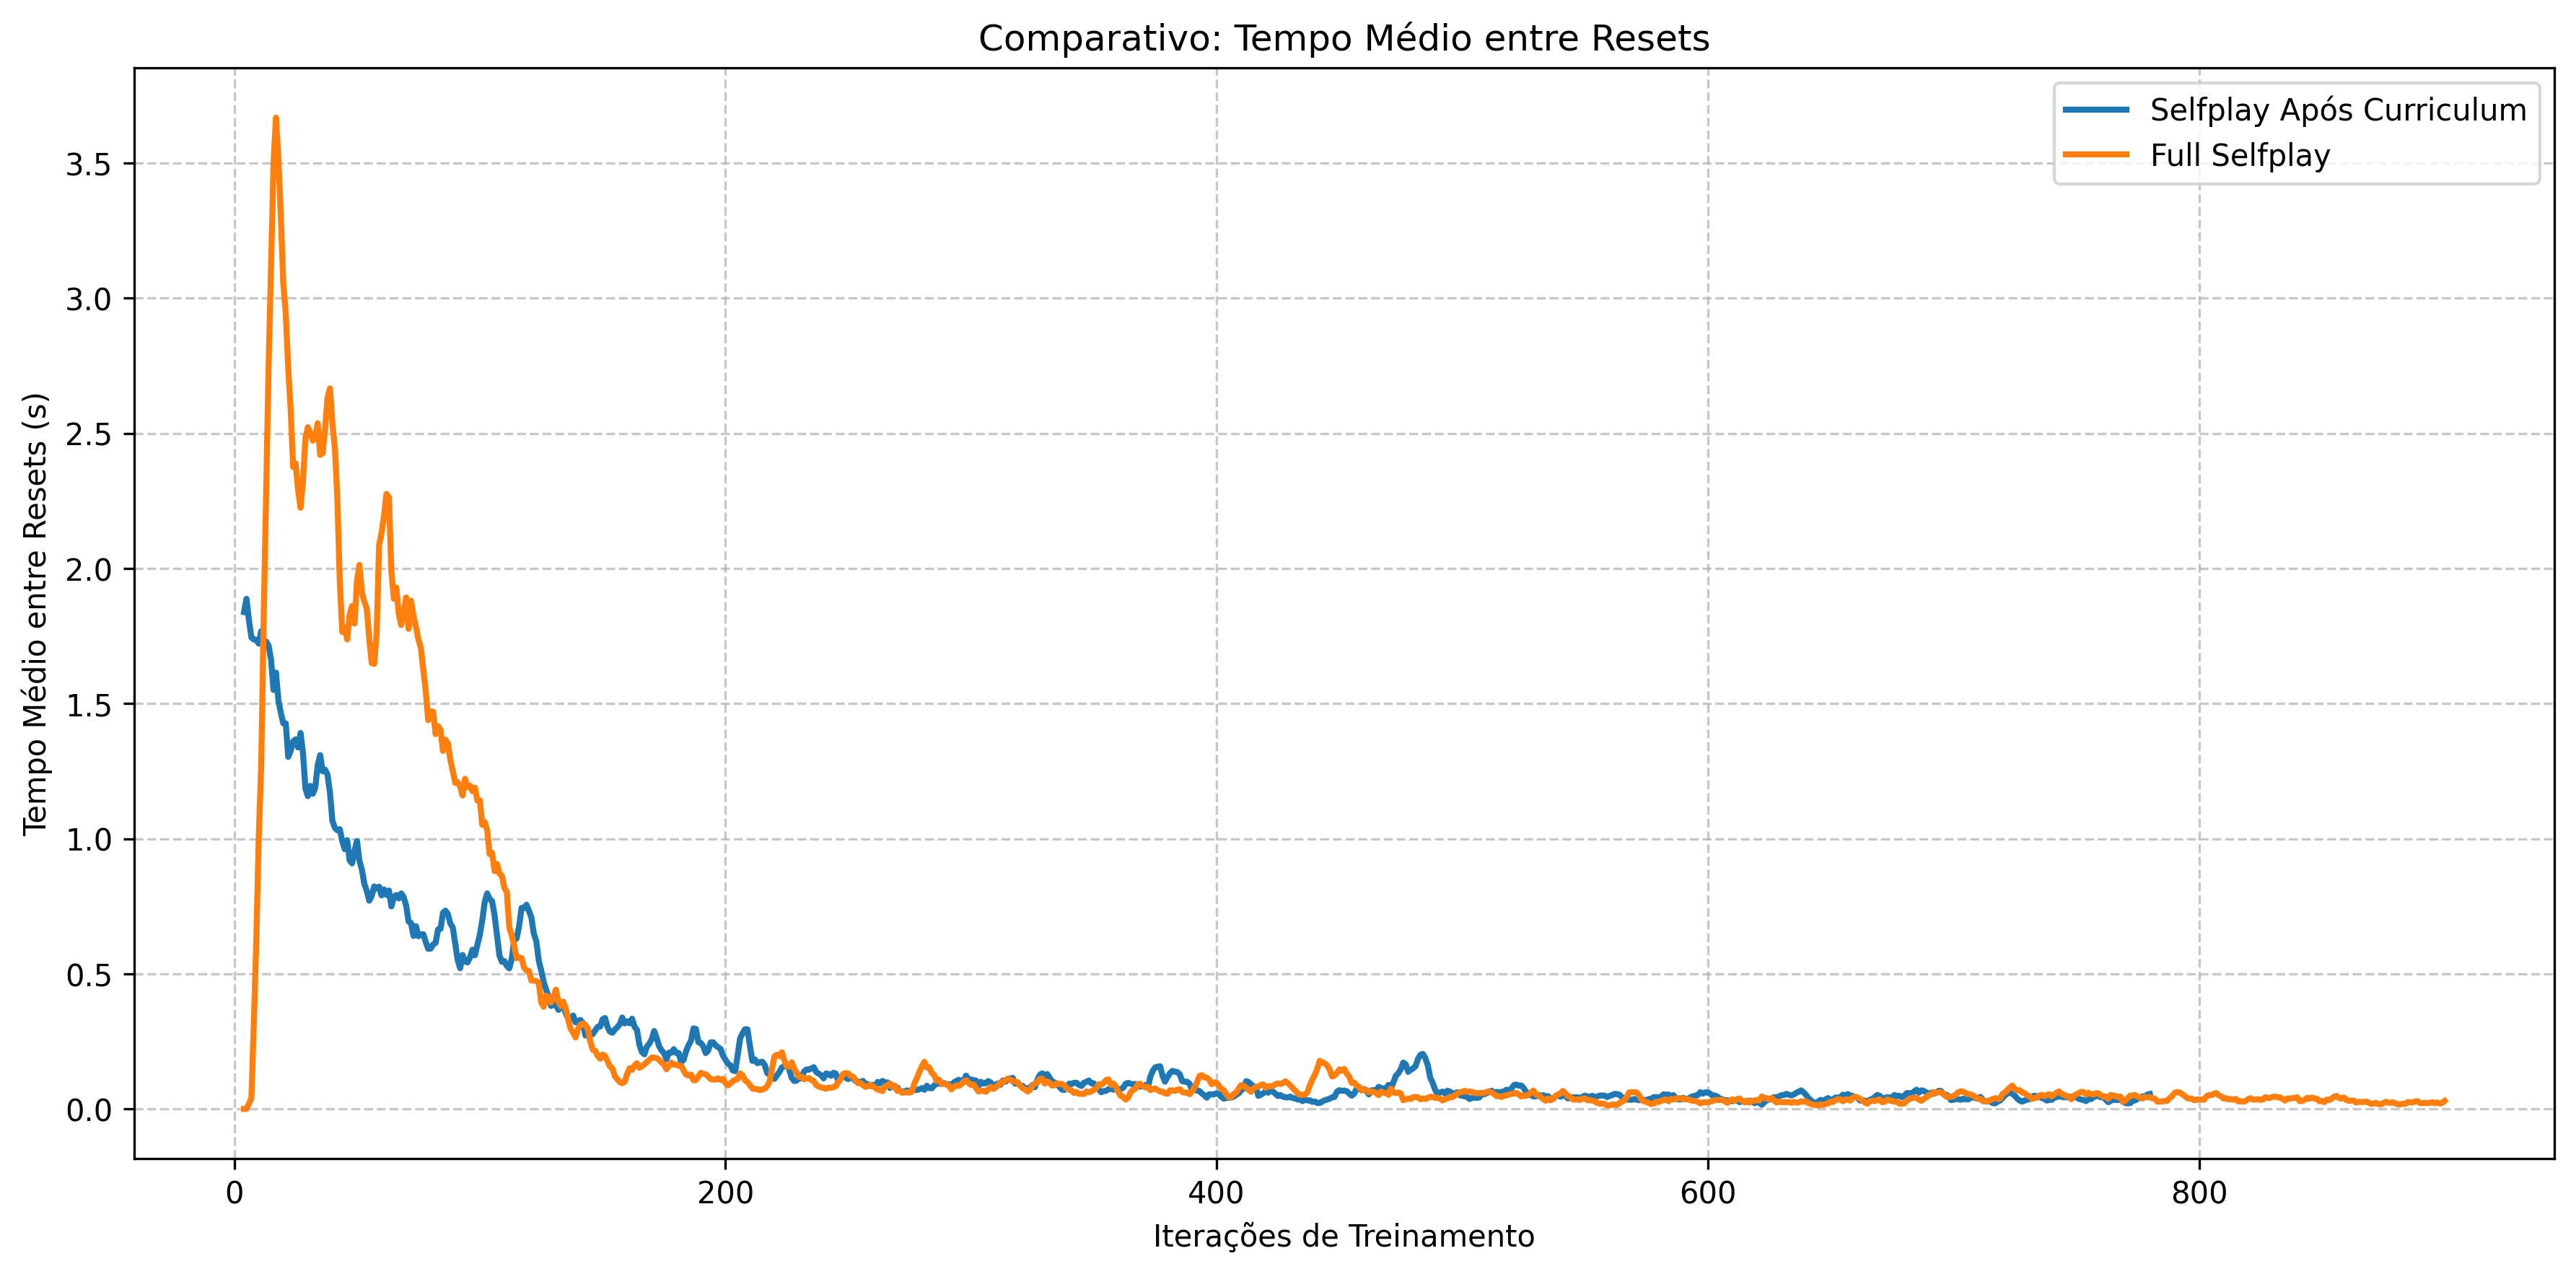
\includegraphics[width=0.95\textwidth]{fig/graficos_trabalho/graficos_experimentos/geral/comparativo_tempo_entre_resets.png}
    \caption{Comparativo do tempo médio entre resets com iterações alinhadas entre as abordagens Selfplay após Curriculum e Full Selfplay}
    \label{fig:time_between_resets}
\end{figure}

O gráfico de tempo médio entre resets mostra tendências inversamente relacionadas ao número de resets, como esperado. Interessantemente, enquanto o Full Selfplay (linha laranja) apresenta inicialmente picos mais altos, indicando períodos mais longos sem interrupções, sua curva de aprendizado para esta métrica é mais lenta e volátil.

O Selfplay após Curriculum demonstra uma curva de aprendizado mais estável, sem os picos extremos, mas com uma progressão mais consistente. Após a iteração 200, ambas as abordagens convergem para valores similares.

Esta análise comparativa com iterações alinhadas demonstra que, embora ambas as abordagens eventualmente atinjam desempenhos similares em termos de continuidade do jogo em suas fases finais, o Selfplay após Curriculum oferece um processo de aprendizado mais eficiente e estável, especialmente durante as fases iniciais e intermediárias do treinamento.

\subsection{Duração dos Episódios}

A análise da duração média dos episódios ao longo do treinamento (Figura \ref{fig:episode_len}) revela padrões interessantes sobre a evolução das estratégias desenvolvidas pelos agentes.

\begin{figure}[H]
    \centering
    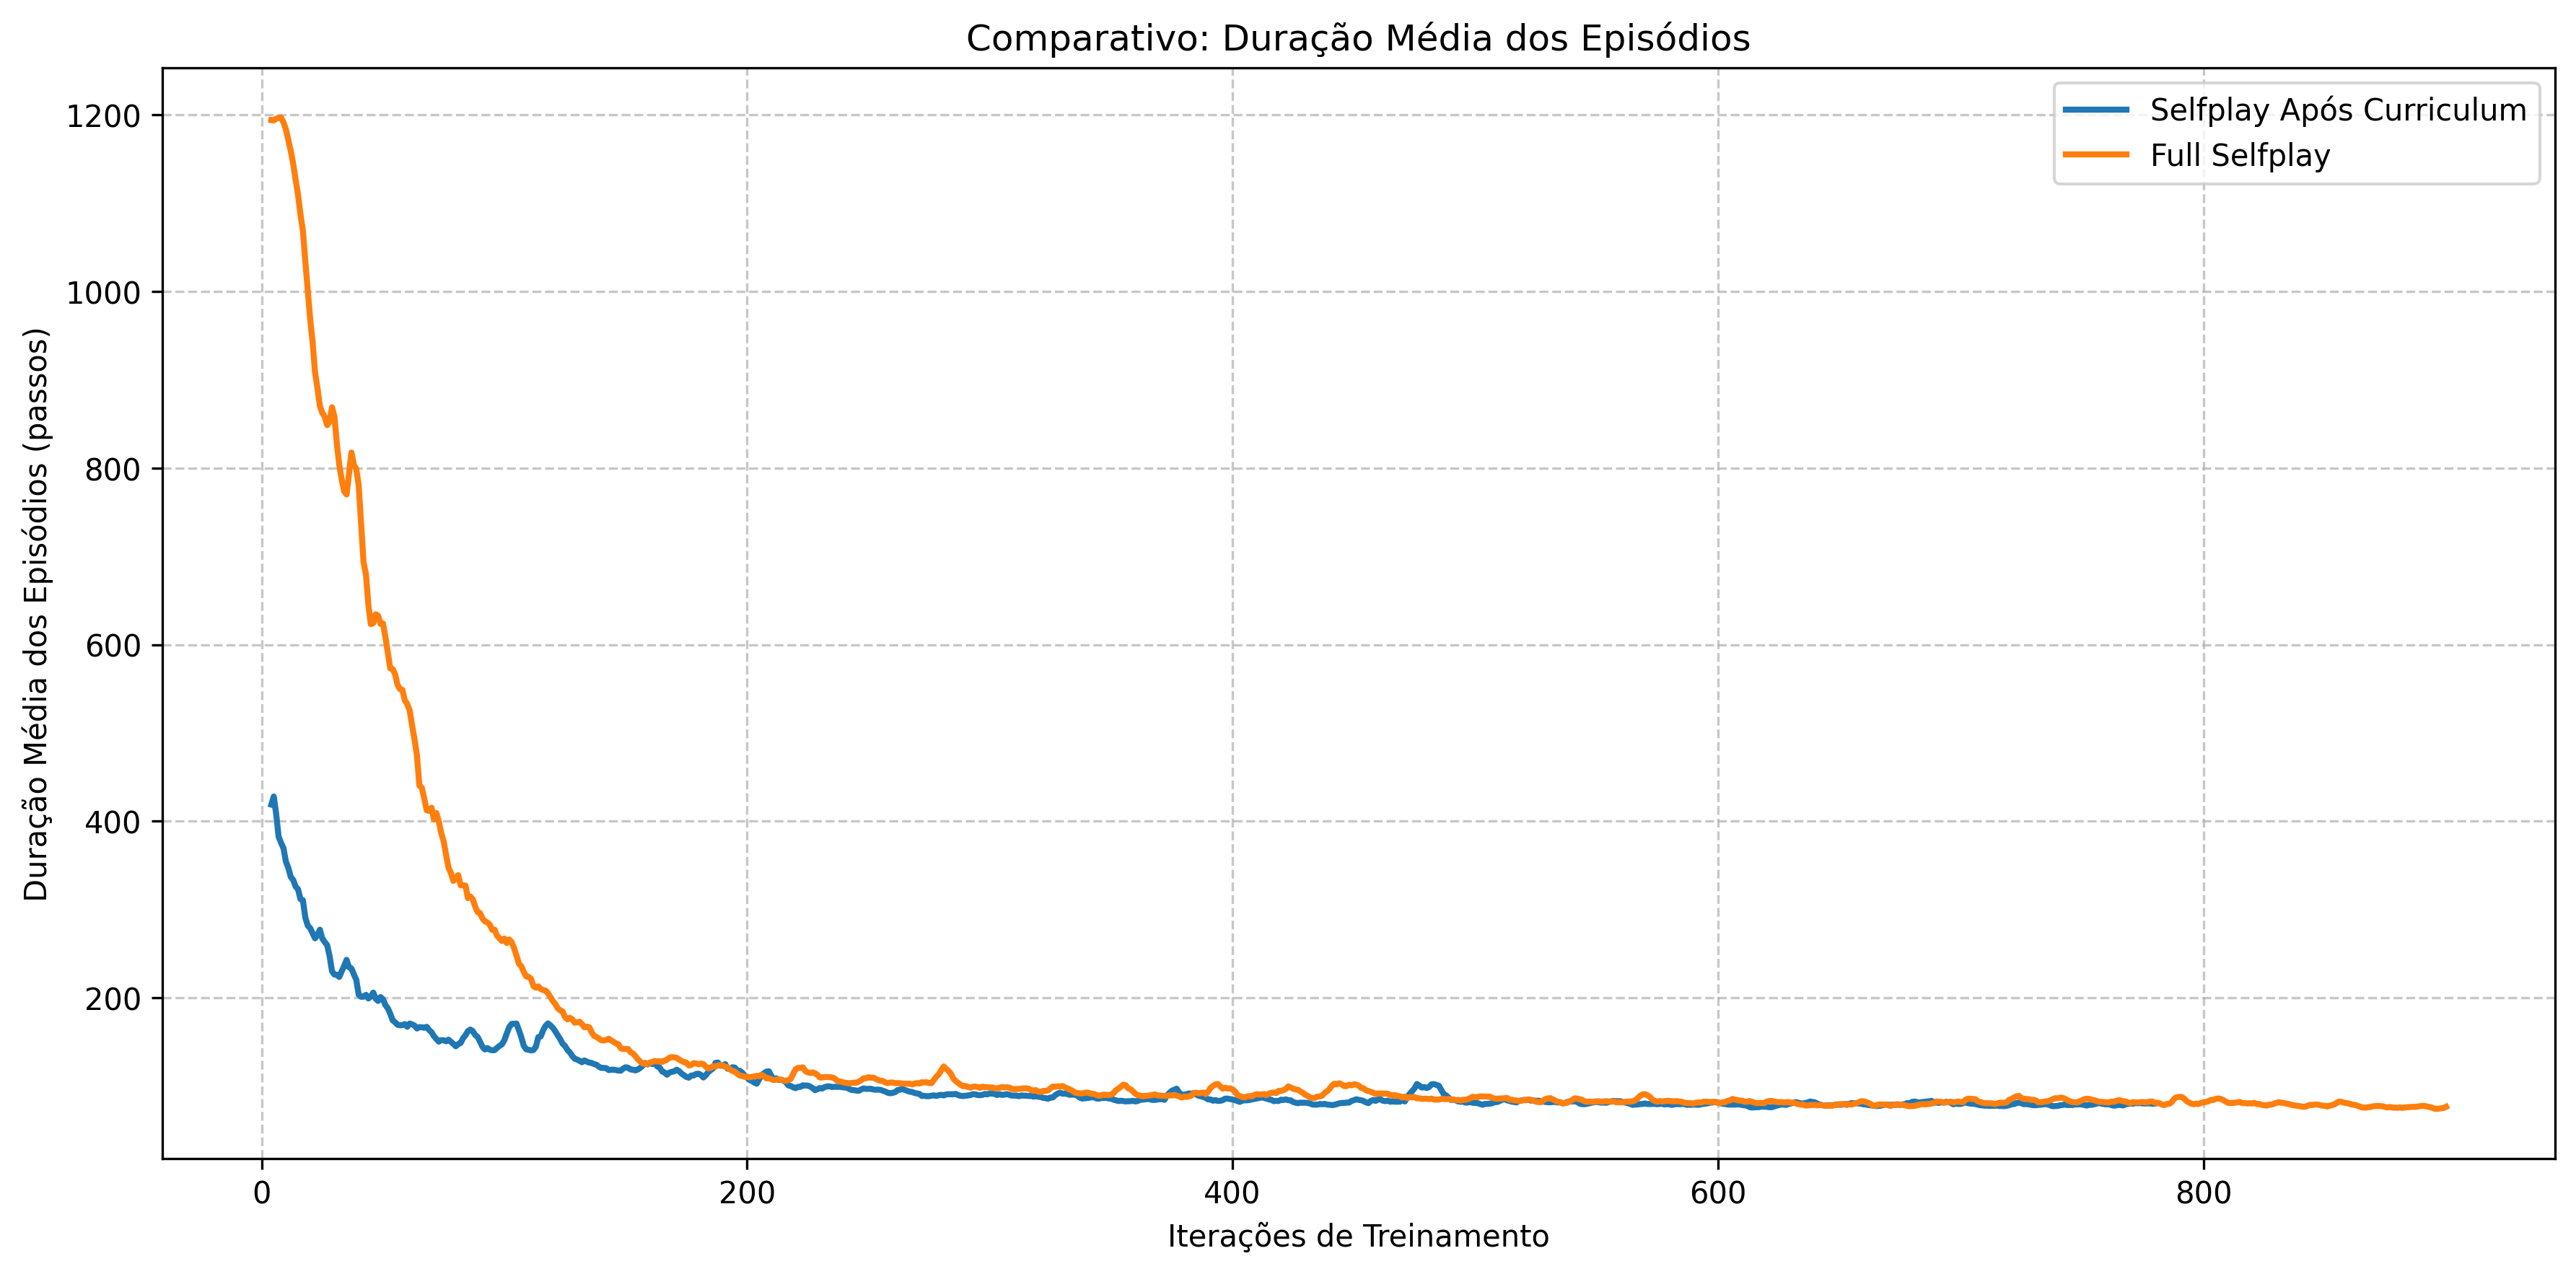
\includegraphics[width=0.95\textwidth]{fig/graficos_trabalho/graficos_experimentos/geral/comparativo_duracao_episodios.png}
    \caption{Comparativo da duração média dos episódios com iterações alinhadas entre as abordagens Selfplay após Curriculum e Full Selfplay}
    \label{fig:episode_len}
\end{figure}

A análise do gráfico revela diferenças marcantes no comportamento dos agentes em relação à duração dos episódios. O Full Selfplay (linha laranja) inicia com episódios significativamente mais longos, atingindo aproximadamente 1200 passos nas primeiras iterações, enquanto o Selfplay após Curriculum (linha azul) começa com episódios bem mais curtos, em torno de 400 passos. Esta diferença inicial demonstra que as habilidades adquiridas durante as fases de curriculum proporcionam um ponto de partida mais eficiente, permitindo aos agentes atingir seus objetivos em menos passos desde o início.

Ao longo do treinamento, ambas as abordagens apresentam uma redução gradual na duração dos episódios, convergindo para valores similares após aproximadamente 200 iterações, quando estabilizam em torno de 100 passos por episódio. Esta redução na duração dos episódios é um indicador positivo, pois demonstra que os agentes estão se tornando mais eficientes em marcar gols, já que cada episódio é encerrado quando um gol é marcado. É notável que o Selfplay após Curriculum apresenta uma curva de aprendizado mais suave e consistente, sem as oscilações pronunciadas observadas no Full Selfplay, indicando um processo de aprendizagem mais estável e uma evolução mais consistente na capacidade de finalização. Nas iterações finais, ambas as abordagens mantêm desempenho similar em termos de velocidade para marcar gols, mas o caminho percorrido pelo Selfplay após Curriculum para atingir este patamar demonstra maior eficiência, especialmente nas fases críticas iniciais e intermediárias do treinamento.

\subsection{Avaliação por Torneios}

Para uma avaliação mais abrangente e realista do desempenho dos modelos treinados, foram realizados torneios controlados com 500 partidas cada, utilizando o sistema Arena Serra Dourada, implementado especificamente para este trabalho. Este sistema permitiu a realização de partidas completas com 10 minutos de duração entre agentes treinados por diferentes métodos.

Os torneios foram organizados em dois confrontos distintos:
\begin{itemize}
    \item \textbf{Torneio 1}: Full Selfplay vs Curriculum - 500 partidas entre agentes treinados apenas com self-play e agentes treinados apenas com curriculum learning.
    \item \textbf{Torneio 2}: Full Selfplay vs Curriculum + Selfplay - 500 partidas entre agentes treinados apenas com self-play e agentes treinados com a abordagem combinada (curriculum seguido por self-play).
\end{itemize}

Cada partida tinha duração de 10 minutos e seguia as regras básicas do futebol de robôs, como cobrança de laterais, faltas e contabilização de gols. Esta configuração experimental permitiu avaliar não apenas a eficácia em marcar gols, mas também a estabilidade das políticas aprendidas em jogos completos e a capacidade de adaptação a diferentes situações de jogo.

A Tabela \ref{tab:resultados_torneios} apresenta um resumo dos resultados dos dois torneios realizados.

\begin{table}[H]
    \centering
    \begin{tabular}{|c|c|c|c|c|c|}
        \hline
        \textbf{Torneio} & \textbf{Partidas} & \textbf{Equipe} & \textbf{Vitórias} & \textbf{Gols} & \textbf{Empates} \\
        \hline
        Torneio 1 & \multicolumn{1}{c|}{500} & Full Selfplay & 247 (49,4\%) & 503 & \multicolumn{1}{c|}{220 (44\%)} \\
        \cline{3-5}
        & & Curriculum & 33 (6,6\%) & 58 & \\
        \hline
        Torneio 2 & \multicolumn{1}{c|}{500} & Full Selfplay & 7 (1,4\%) & 9 & \multicolumn{1}{c|}{63 (12,6\%)} \\
        \cline{3-5}
        & & Curriculum + Selfplay & 430 (86\%) & 1012 & \\
        \hline
    \end{tabular}
    \caption{Resumo dos resultados dos torneios realizados com 500 partidas cada}
    \label{tab:resultados_torneios}
\end{table}

Os resultados revelam padrões interessantes sobre o desempenho de cada abordagem. No Torneio 1 (Full Selfplay vs Curriculum), observamos uma clara superioridade do modelo treinado apenas com self-play, que obteve 247 vitórias (49,4\%) contra apenas 33 vitórias (6,6\%) do modelo treinado somente com curriculum learning. É notável também o alto número de empates (220, correspondendo a 44\% dos jogos), sugerindo que o modelo de curriculum, apesar de seu desempenho inferior em termos de vitórias, desenvolveu capacidades defensivas significativas.

No Torneio 2 (Full Selfplay vs Curriculum + Selfplay), os resultados evidenciam a esmagadora superioridade do modelo treinado com a combinação de curriculum learning e self-play, que obteve 430 vitórias (86\%) em comparação com apenas 7 vitórias (1,4\%) do modelo full self-play. O número de empates foi significativamente menor (63, apenas 12,6\% dos jogos), indicando partidas mais decisivas e menos equilibradas.

Esta diferença dramática no desempenho destaca o poderoso efeito sinérgico obtido ao combinar as duas abordagens. Enquanto o curriculum learning isolado apresenta limitações significativas em um cenário competitivo completo, sua integração com o self-play resulta em políticas substancialmente mais eficazes do que aquelas desenvolvidas apenas com self-play.

\begin{figure}[H]
    \centering
    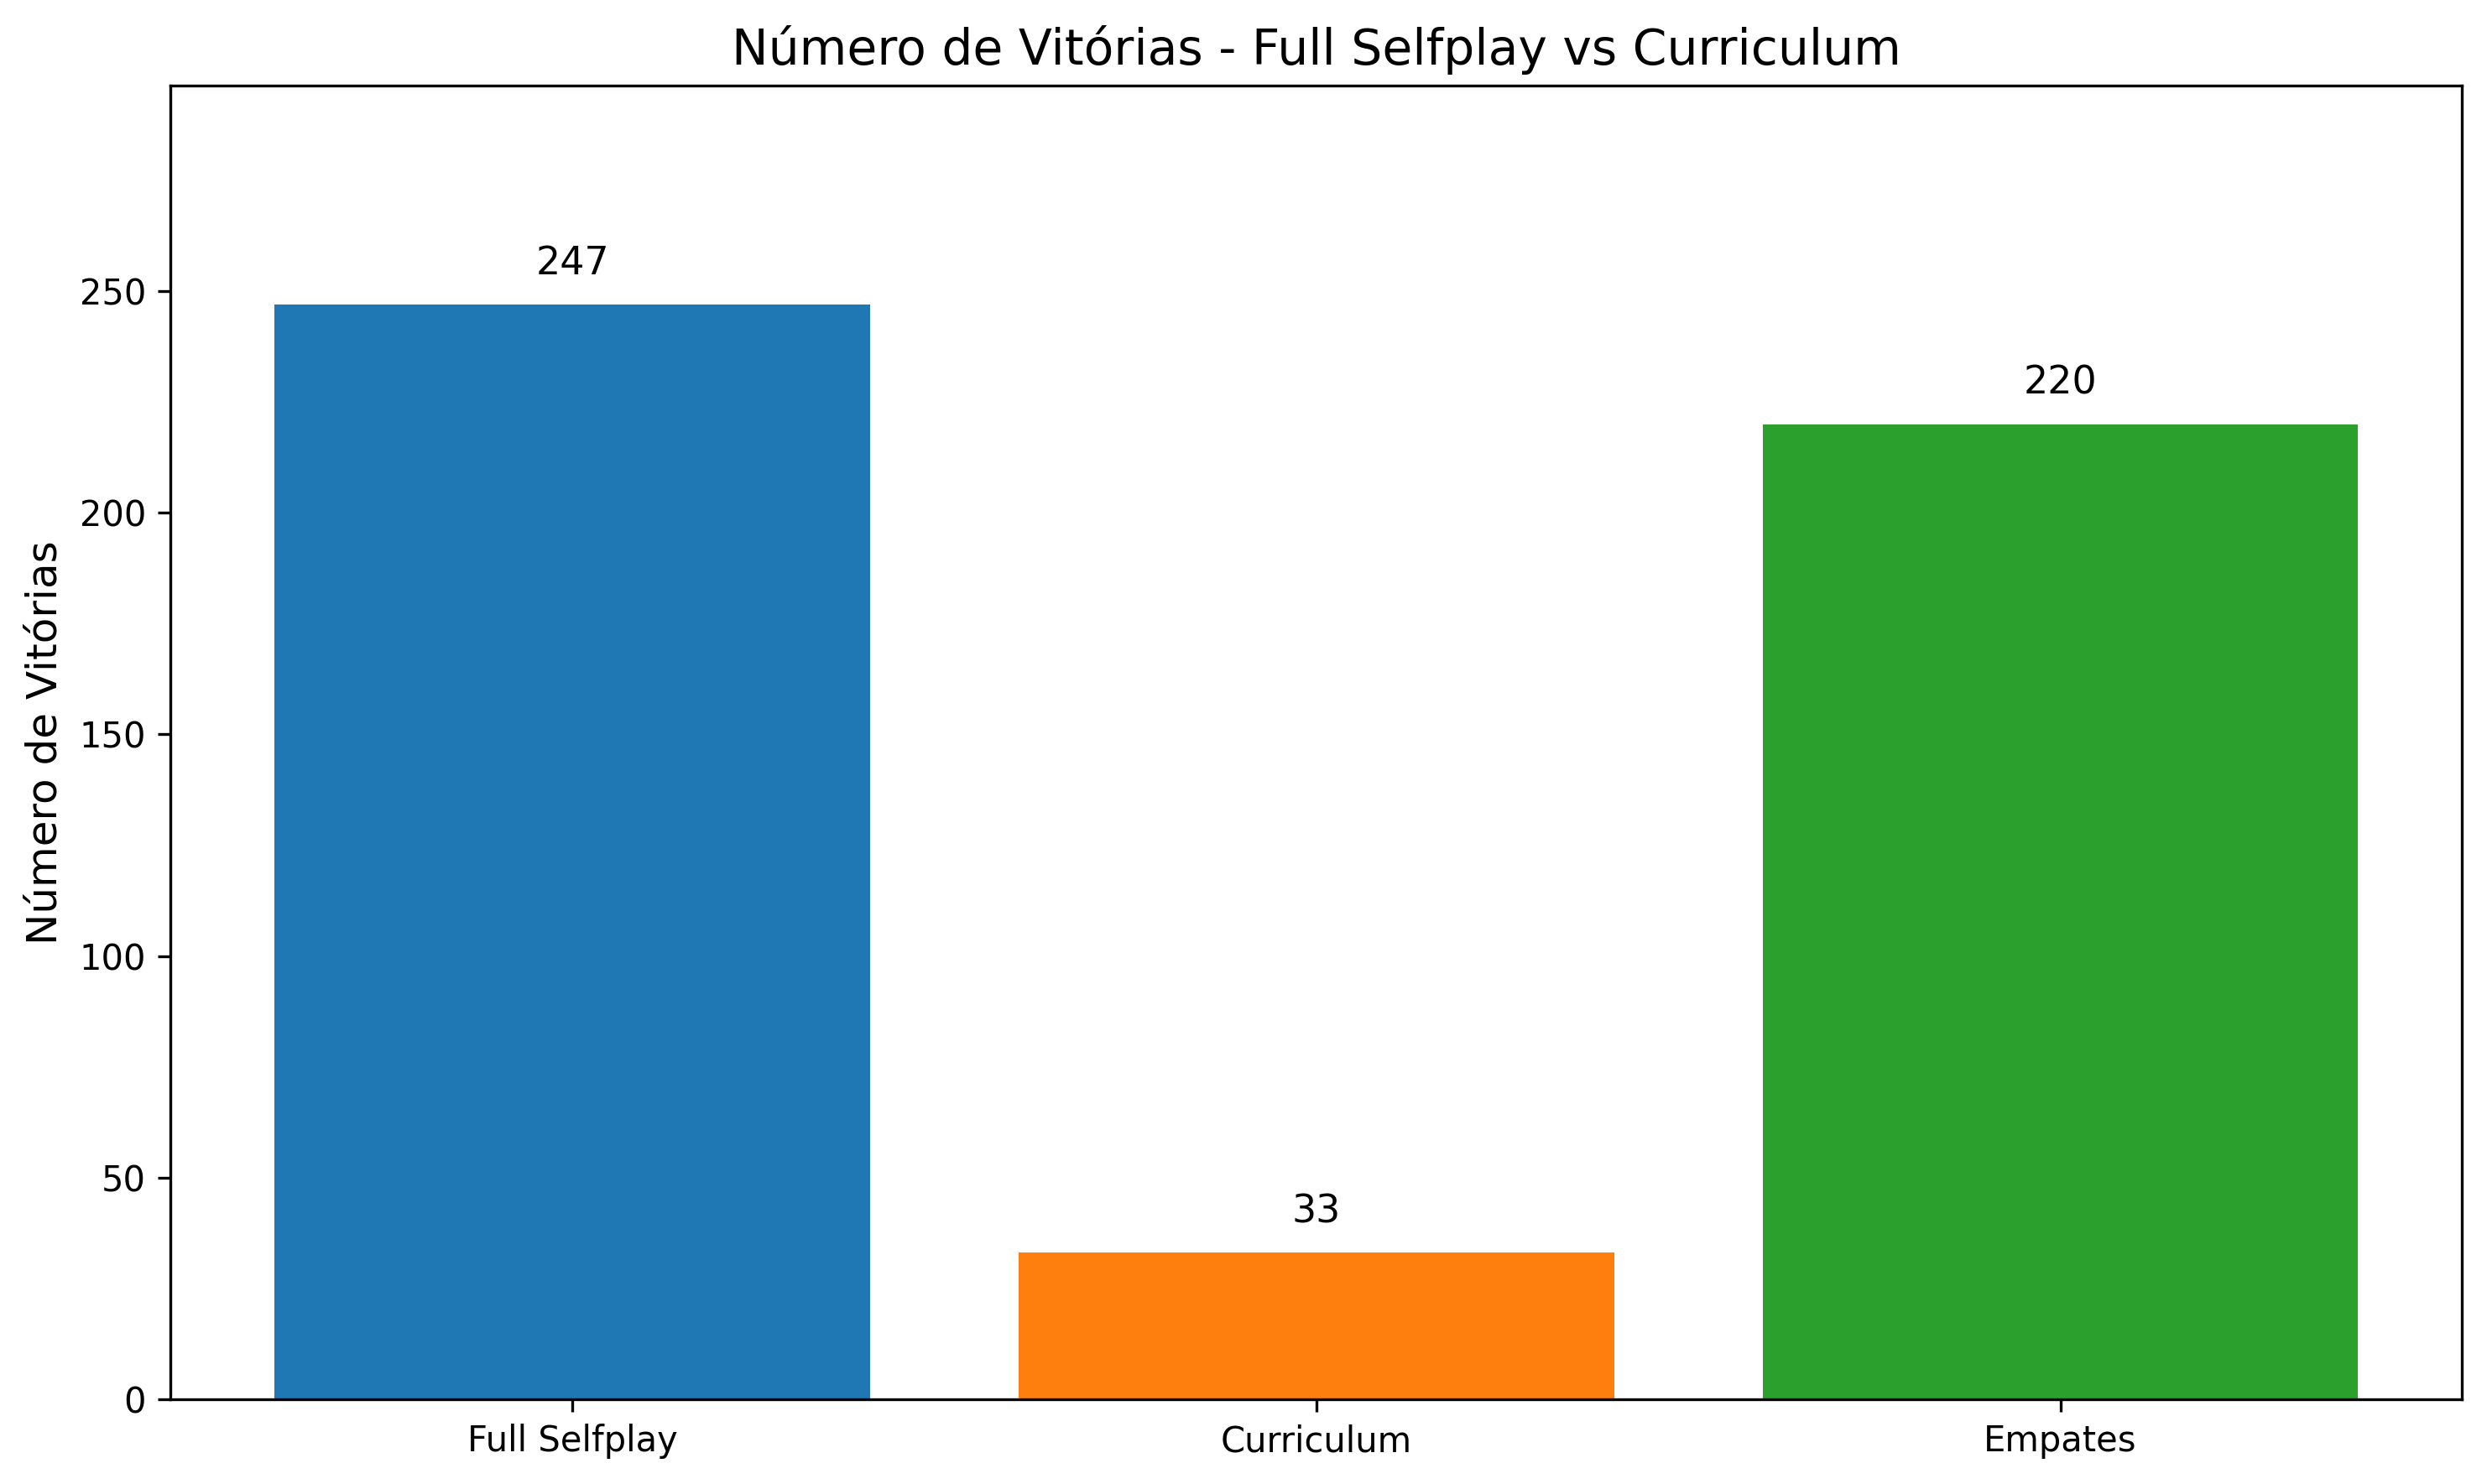
\includegraphics[width=0.8\textwidth]{fig/graficos_trabalho/graficos_torneios/torneios/vitorias_full_selfplay_vs_curriculum.png}
    \caption{Distribuição de resultados no Torneio 1: Full Selfplay vs Curriculum}
    \label{fig:vitorias_torneio1}
\end{figure}

\begin{figure}[H]
    \centering
    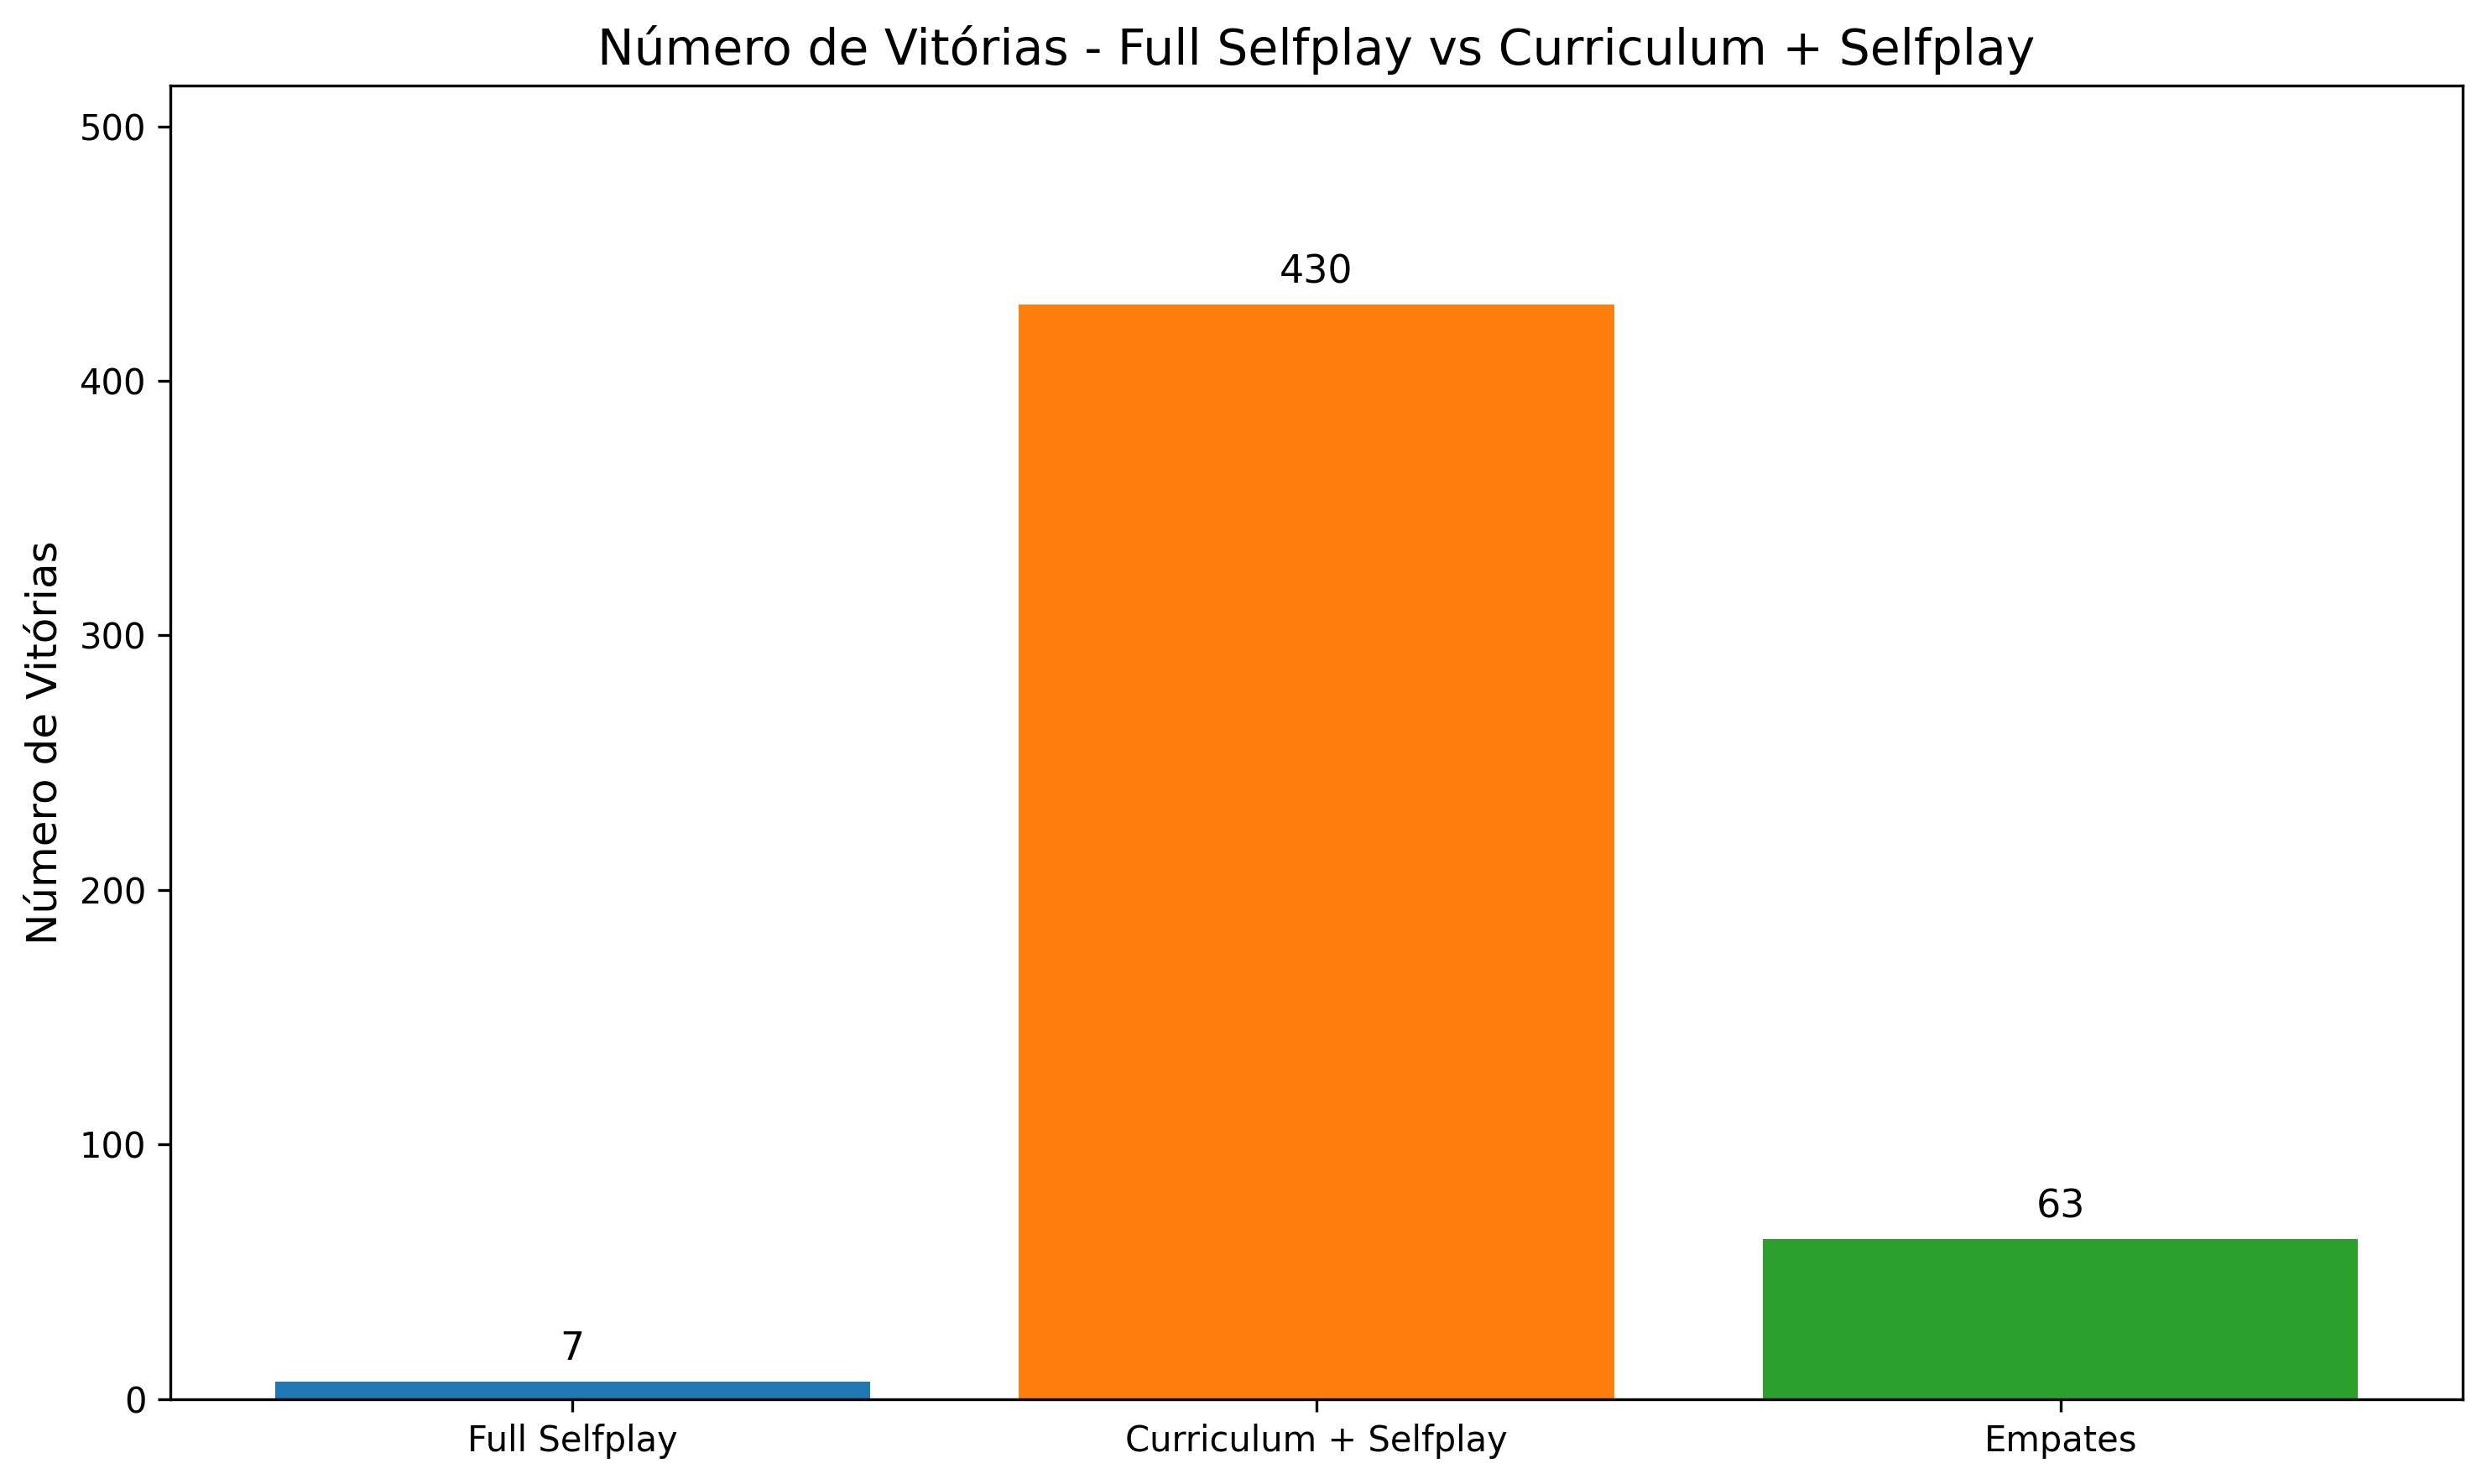
\includegraphics[width=0.8\textwidth]{fig/graficos_trabalho/graficos_torneios/torneios/vitorias_full_selfplay_vs_curriculum_+_selfplay.png}
    \caption{Distribuição de resultados no Torneio 2: Full Selfplay vs Curriculum + Selfplay}
    \label{fig:vitorias_torneio2}
\end{figure}

A comparação visual das Figuras \ref{fig:vitorias_torneio1} e \ref{fig:vitorias_torneio2} evidencia claramente a inversão de desempenho entre os torneios e o impacto transformador da abordagem combinada.

\subsection{Análise de Gols nos Torneios}

Além da taxa de vitória, analisamos também o desempenho ofensivo dos modelos nos torneios realizados, com foco na capacidade de marcar gols, que representa um indicador fundamental de eficácia no futebol de robôs.

\begin{figure}[H]
    \centering
    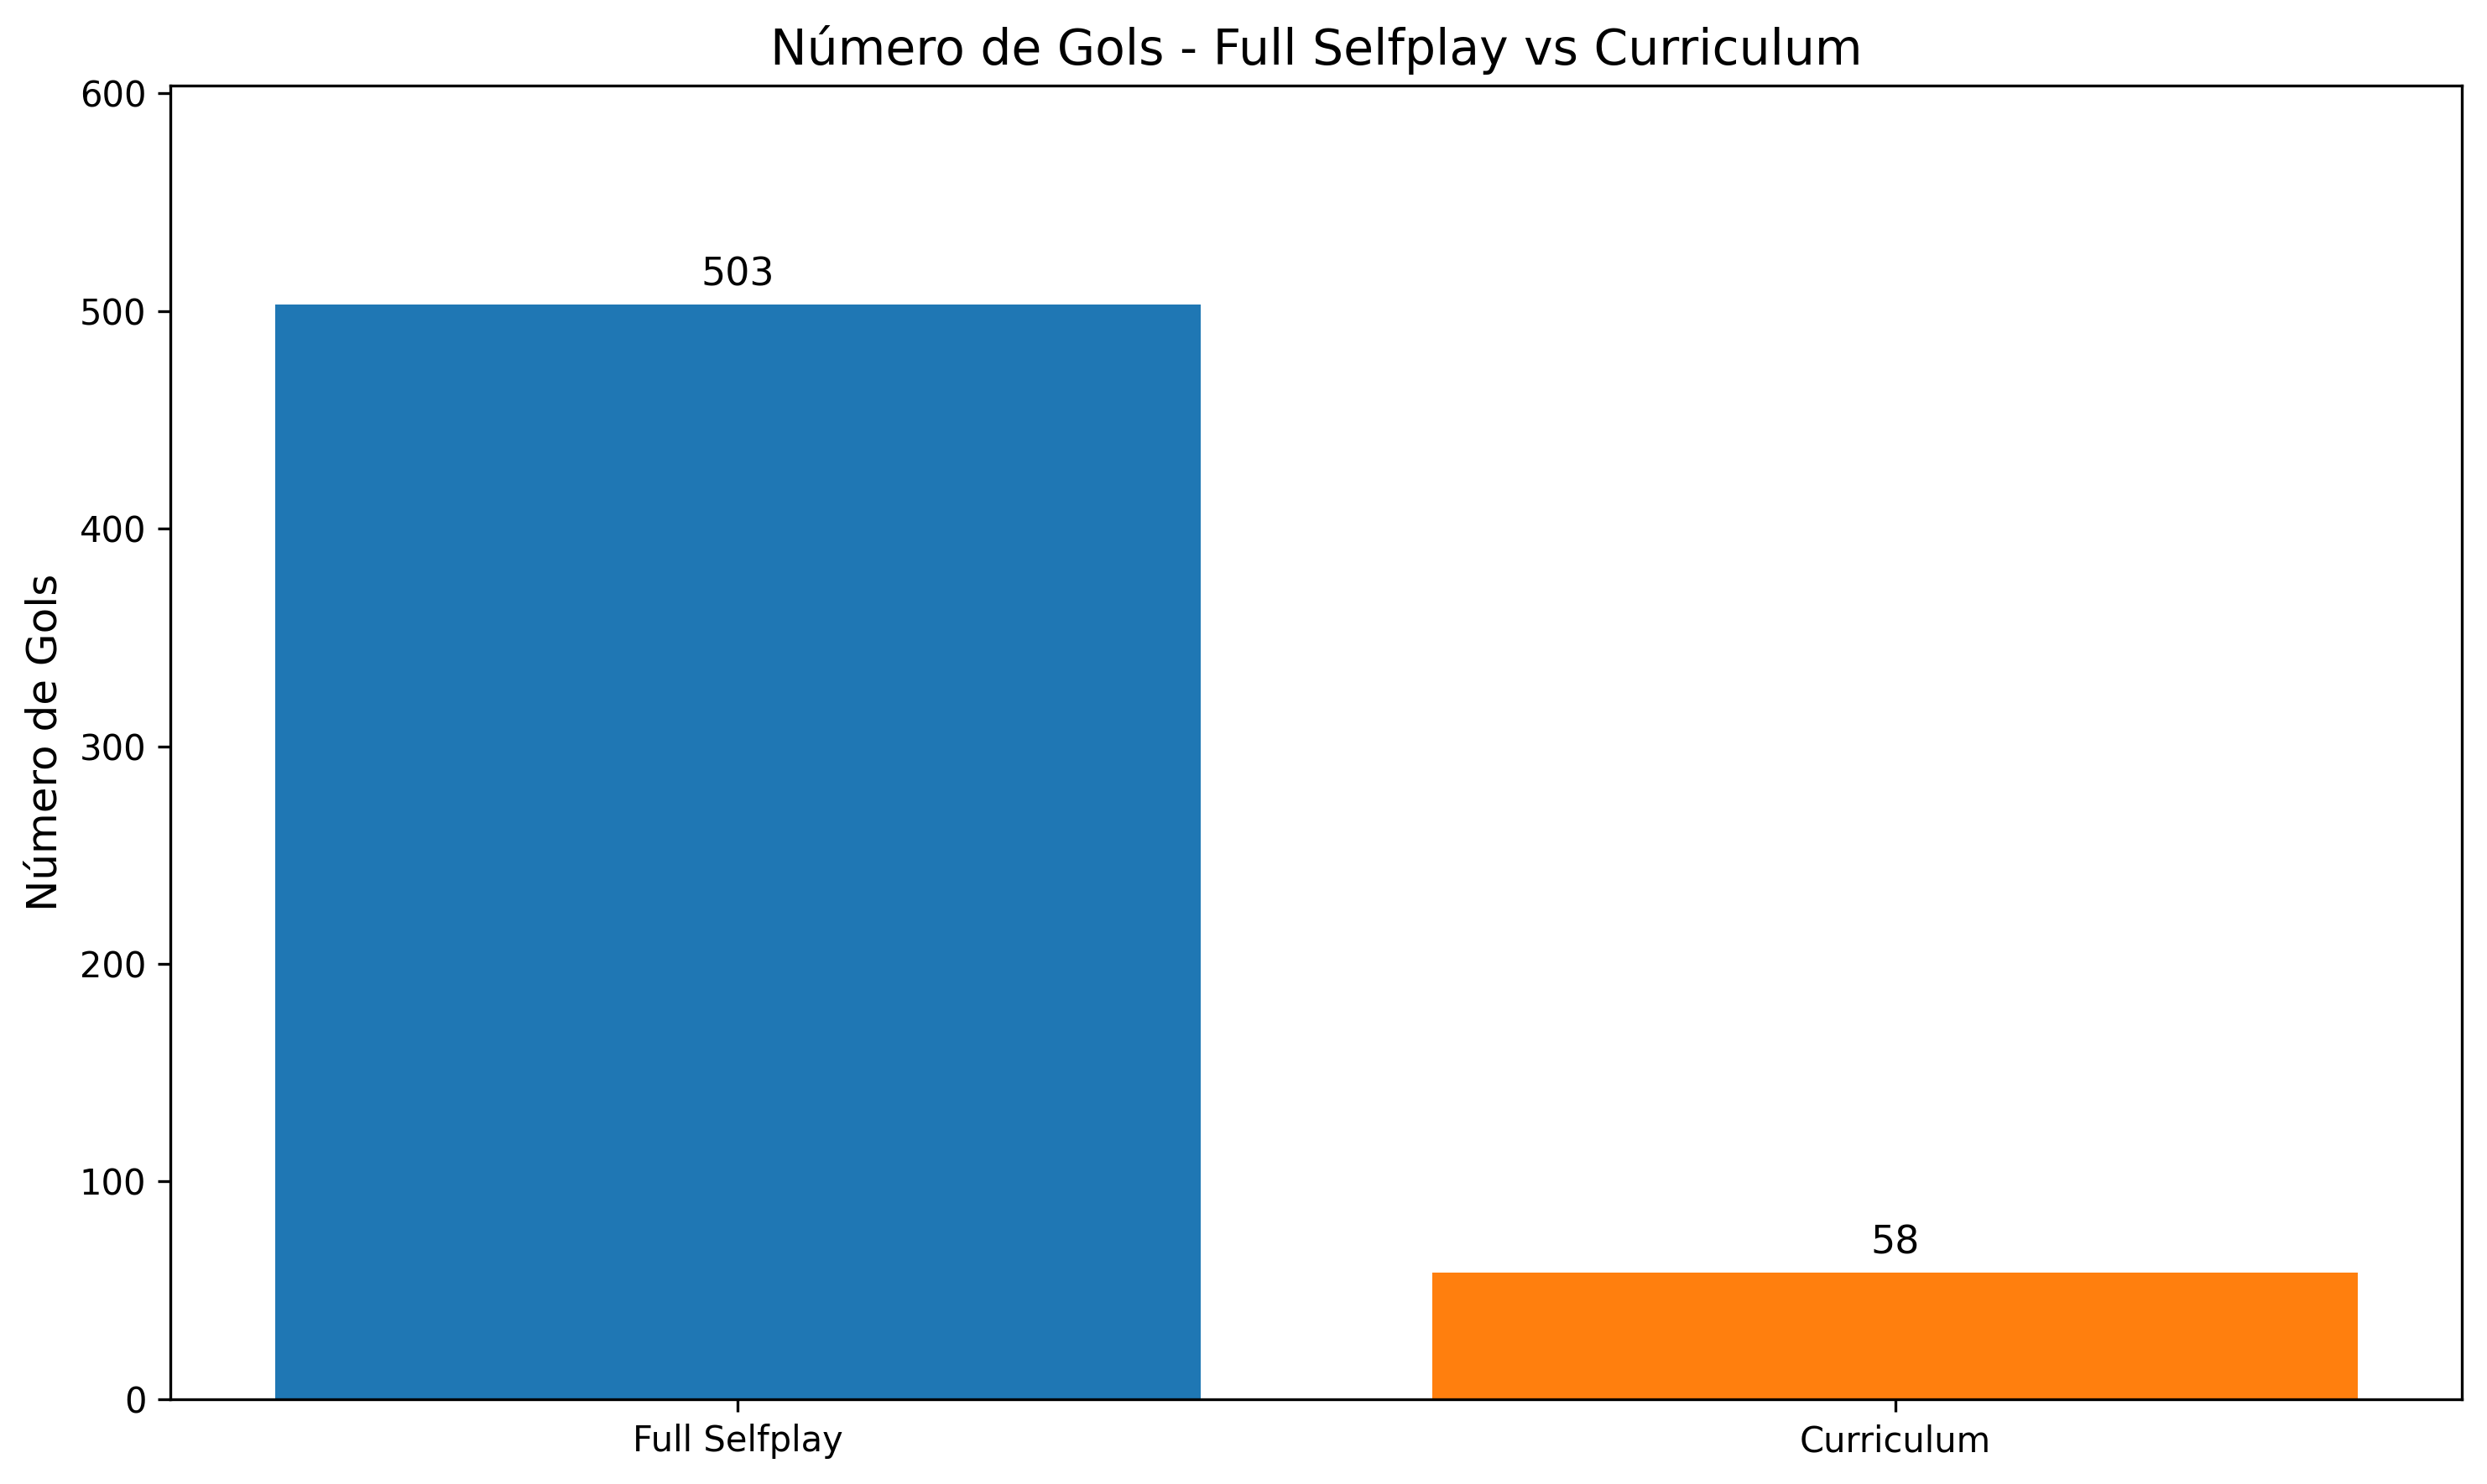
\includegraphics[width=0.8\textwidth]{fig/graficos_trabalho/graficos_torneios/torneios/gols_full_selfplay_vs_curriculum.png}
    \caption{Comparação de gols marcados no Torneio 1: Full Selfplay vs Curriculum}
    \label{fig:gols_torneio1}
\end{figure}

\begin{figure}[H]
    \centering
    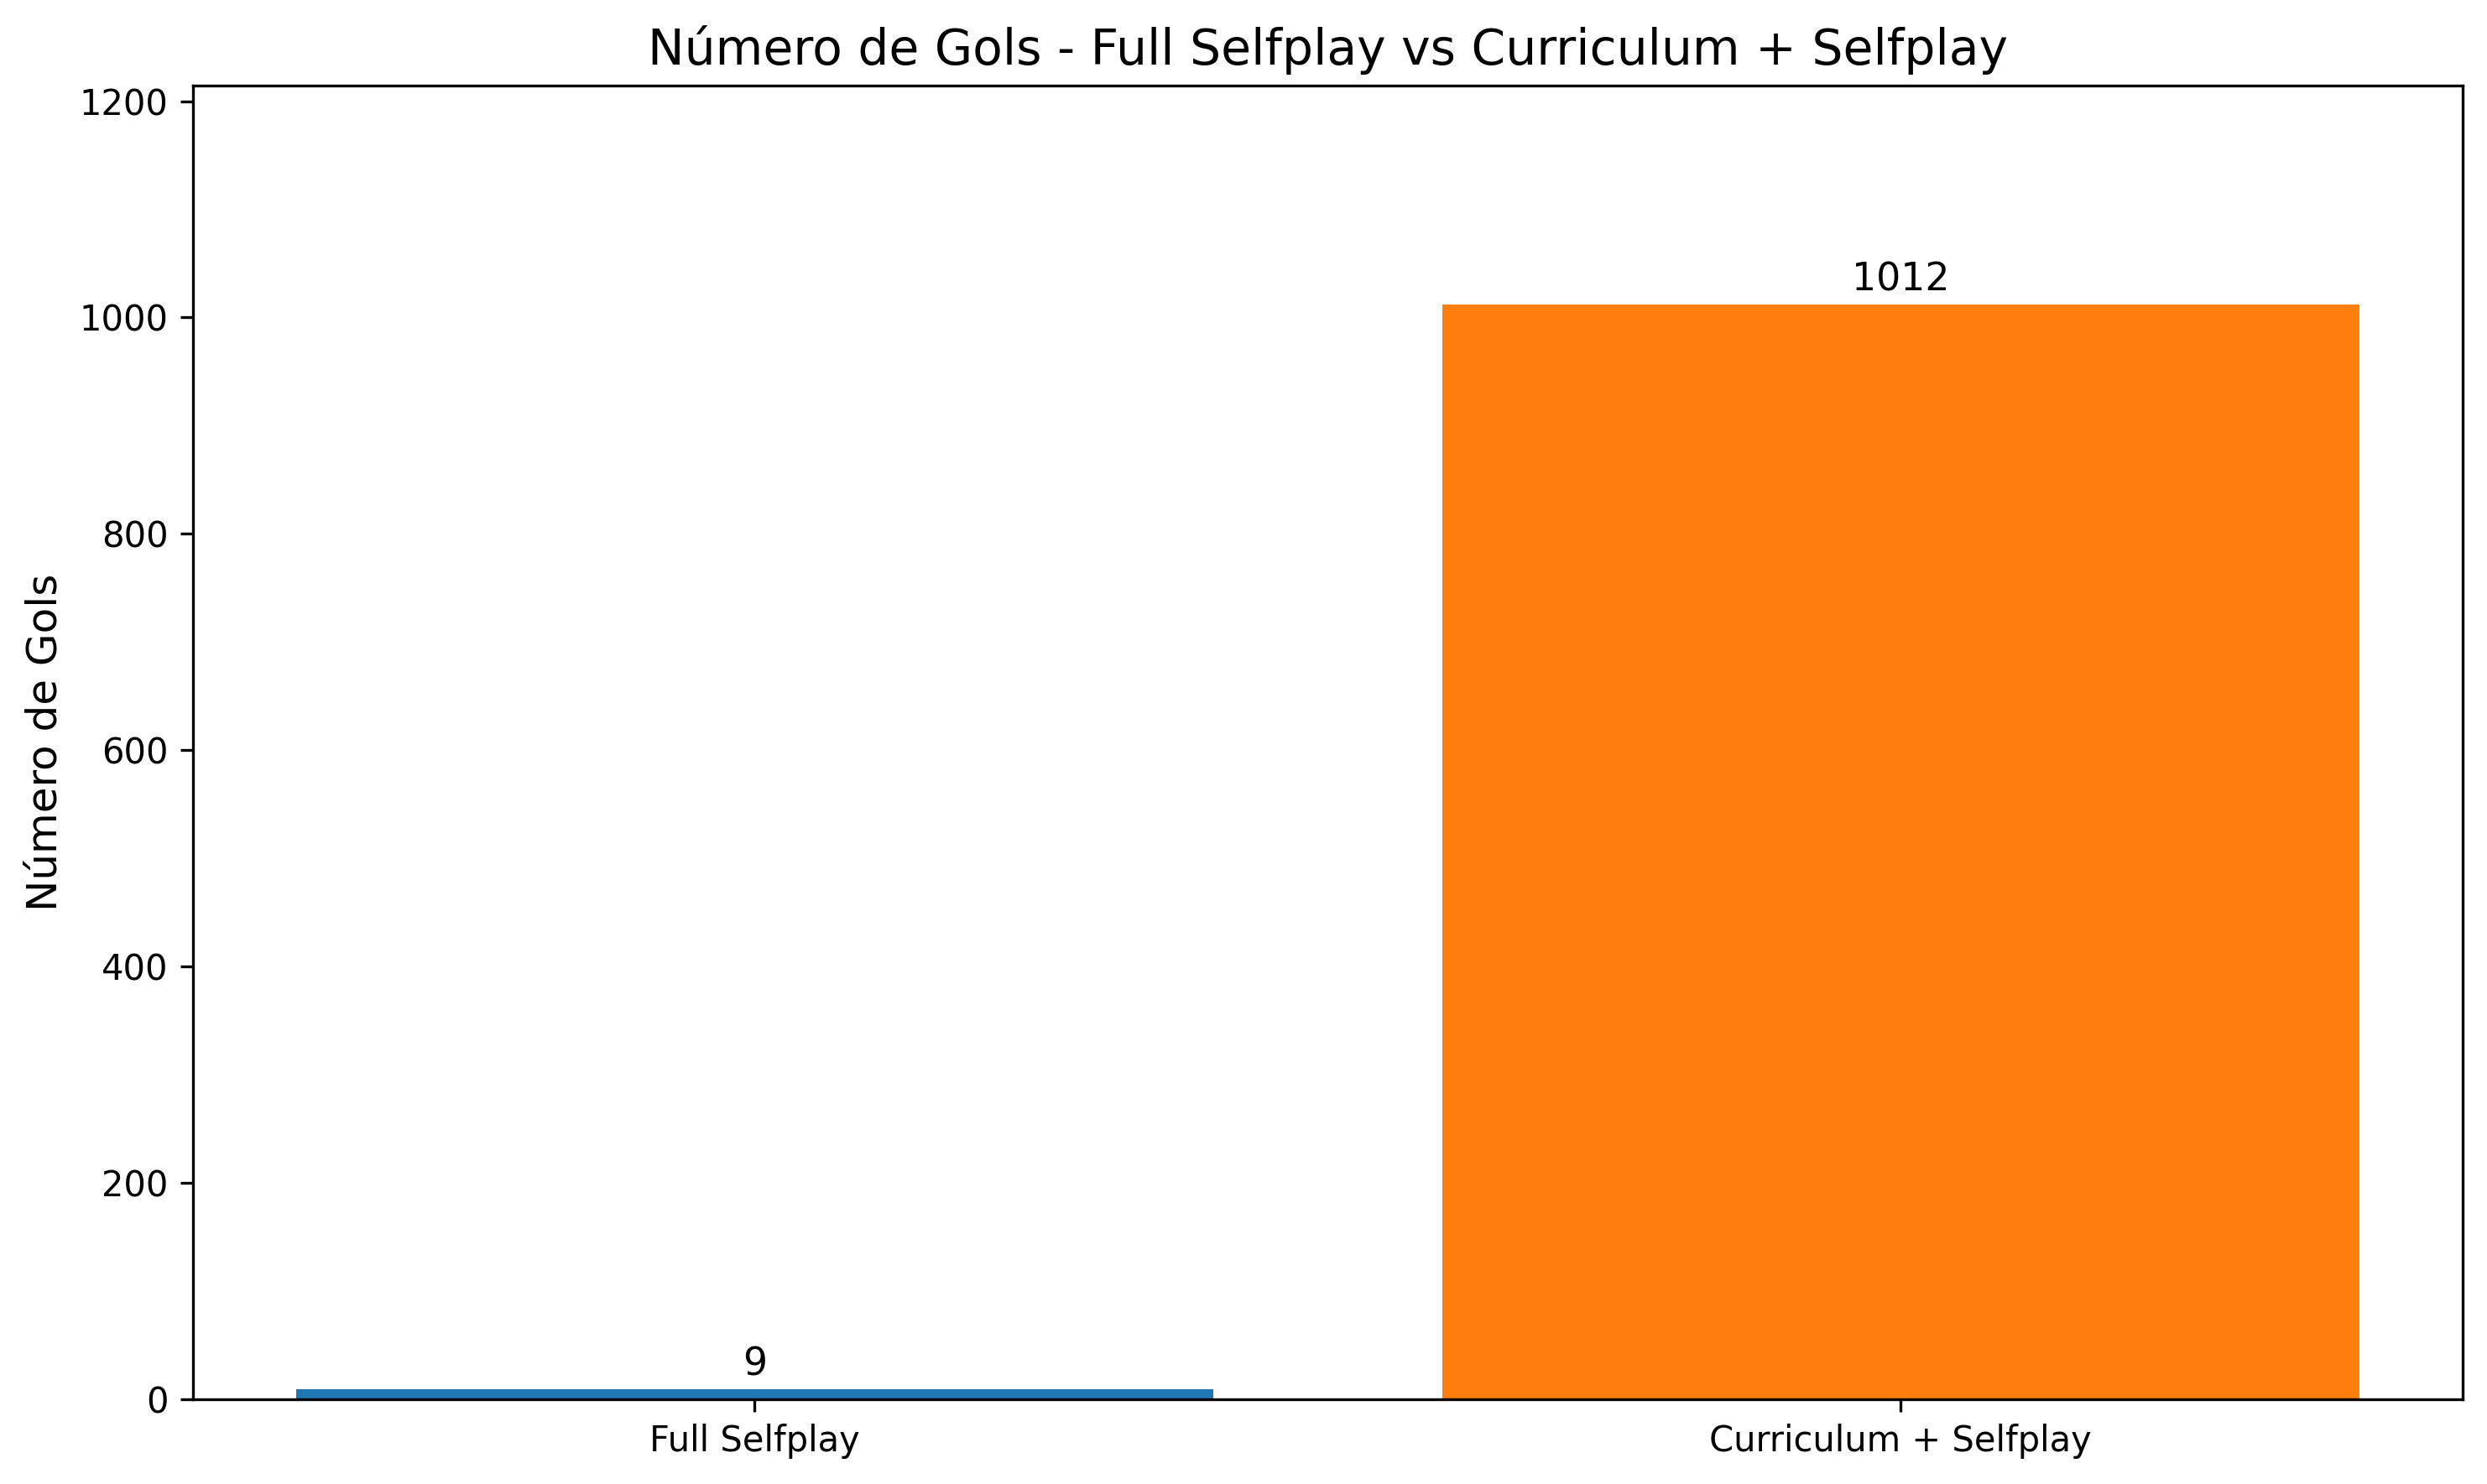
\includegraphics[width=0.8\textwidth]{fig/graficos_trabalho/graficos_torneios/torneios/gols_full_selfplay_vs_curriculum_+_selfplay.png}
    \caption{Comparação de gols marcados no Torneio 2: Full Selfplay vs Curriculum + Selfplay}
    \label{fig:gols_torneio2}
\end{figure}

A análise dos gols marcados em cada torneio revela padrões consistentes com os resultados gerais das partidas, mas com diferenças de magnitude ainda mais pronunciadas.

No Torneio 1 (Full Selfplay vs Curriculum), o modelo treinado apenas com self-play demonstrou capacidade ofensiva significativamente superior, marcando 503 gols durante as 500 partidas, o que corresponde a uma média de 1,006 gols por partida. Em contraste, o modelo treinado exclusivamente com curriculum learning marcou apenas 58 gols (média de 0,116 por partida), aproximadamente 11,5\% do desempenho ofensivo do Full Selfplay.

Esta disparidade sugere que, embora o curriculum learning desenvolva habilidades fundamentais, ele não é suficiente para criar agentes com capacidade ofensiva efetiva em um cenário competitivo completo. A limitação ofensiva explica o alto número de empates e a baixa taxa de vitórias do modelo Curriculum.

No Torneio 2 (Full Selfplay vs Curriculum + Selfplay), observamos uma inversão dramática deste padrão. O modelo combinado (curriculum + self-play) apresentou uma capacidade ofensiva extraordinária, marcando 1.012 gols durante as 500 partidas, o que corresponde a uma impressionante média de 2,024 gols por partida. Em contraste, o modelo Full Selfplay marcou apenas 9 gols (média de 0,018 por partida), menos de 1\% do desempenho ofensivo do modelo combinado.

\begin{figure}[H]
    \centering
    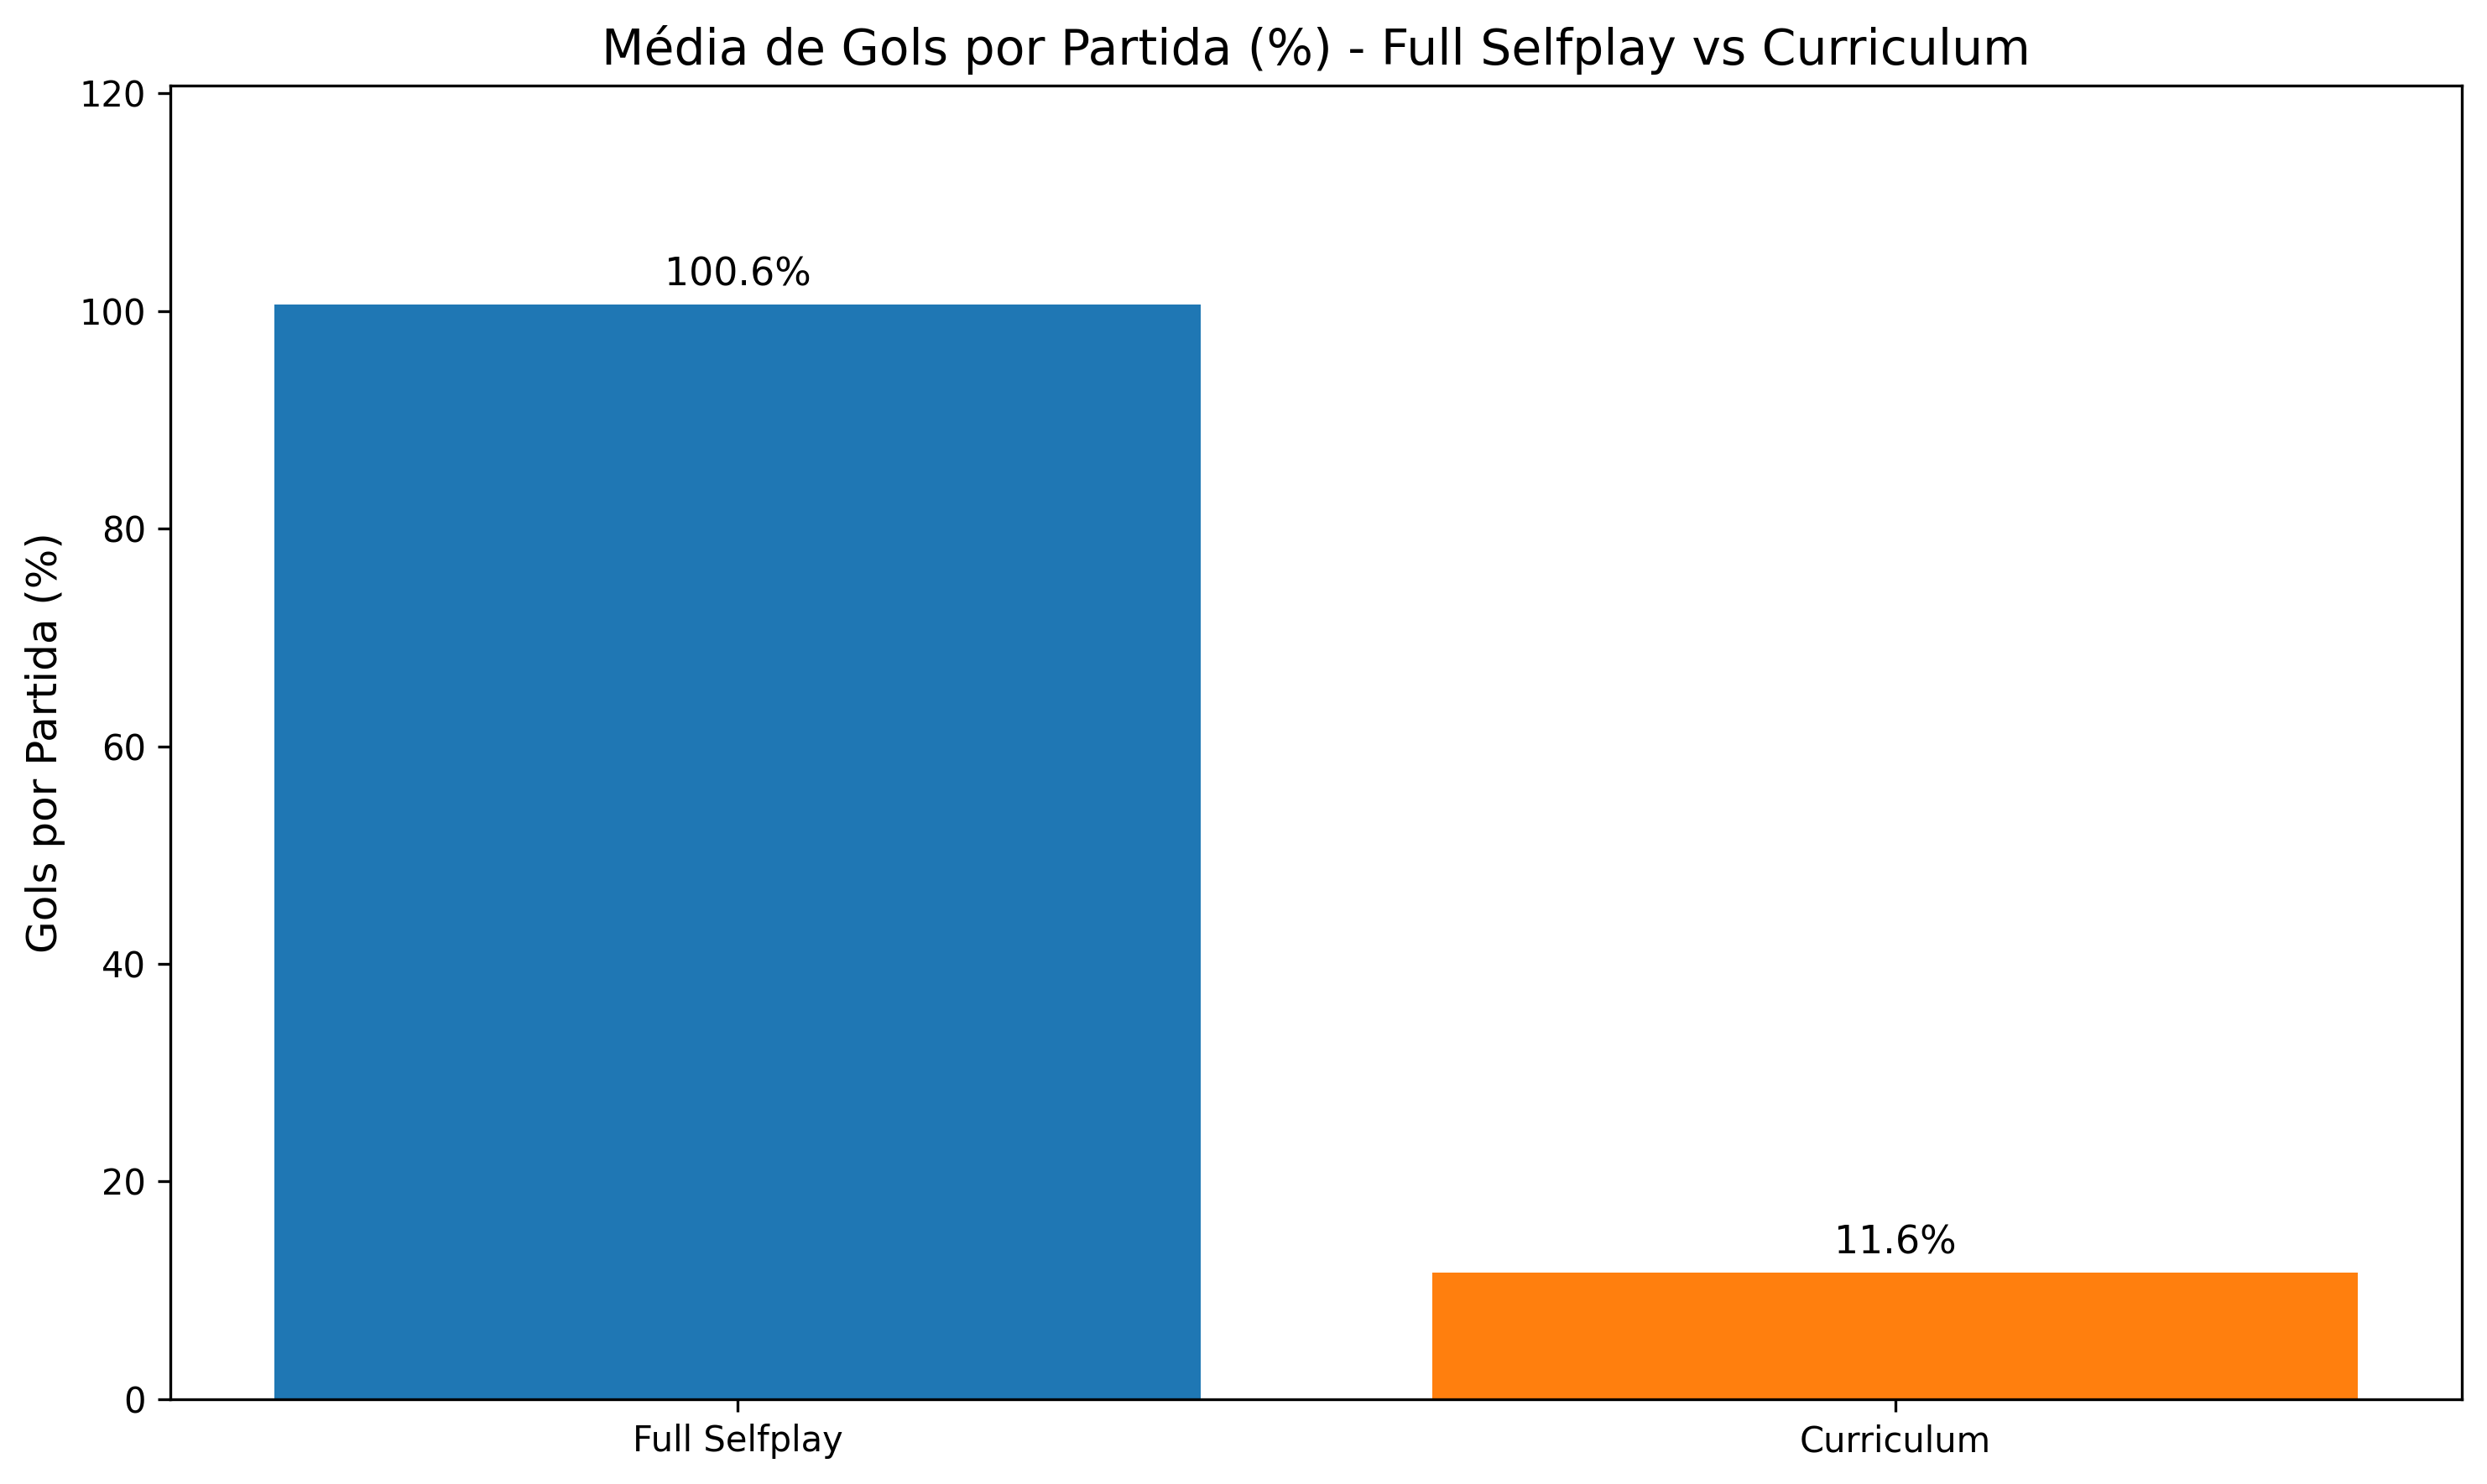
\includegraphics[width=0.8\textwidth]{fig/graficos_trabalho/graficos_torneios/torneios/percentual_gols_full_selfplay_vs_curriculum.png}
    \caption{Percentual de gols no Torneio 1: Full Selfplay vs Curriculum}
    \label{fig:percentual_gols_torneio1}
\end{figure}

\begin{figure}[H]
    \centering
    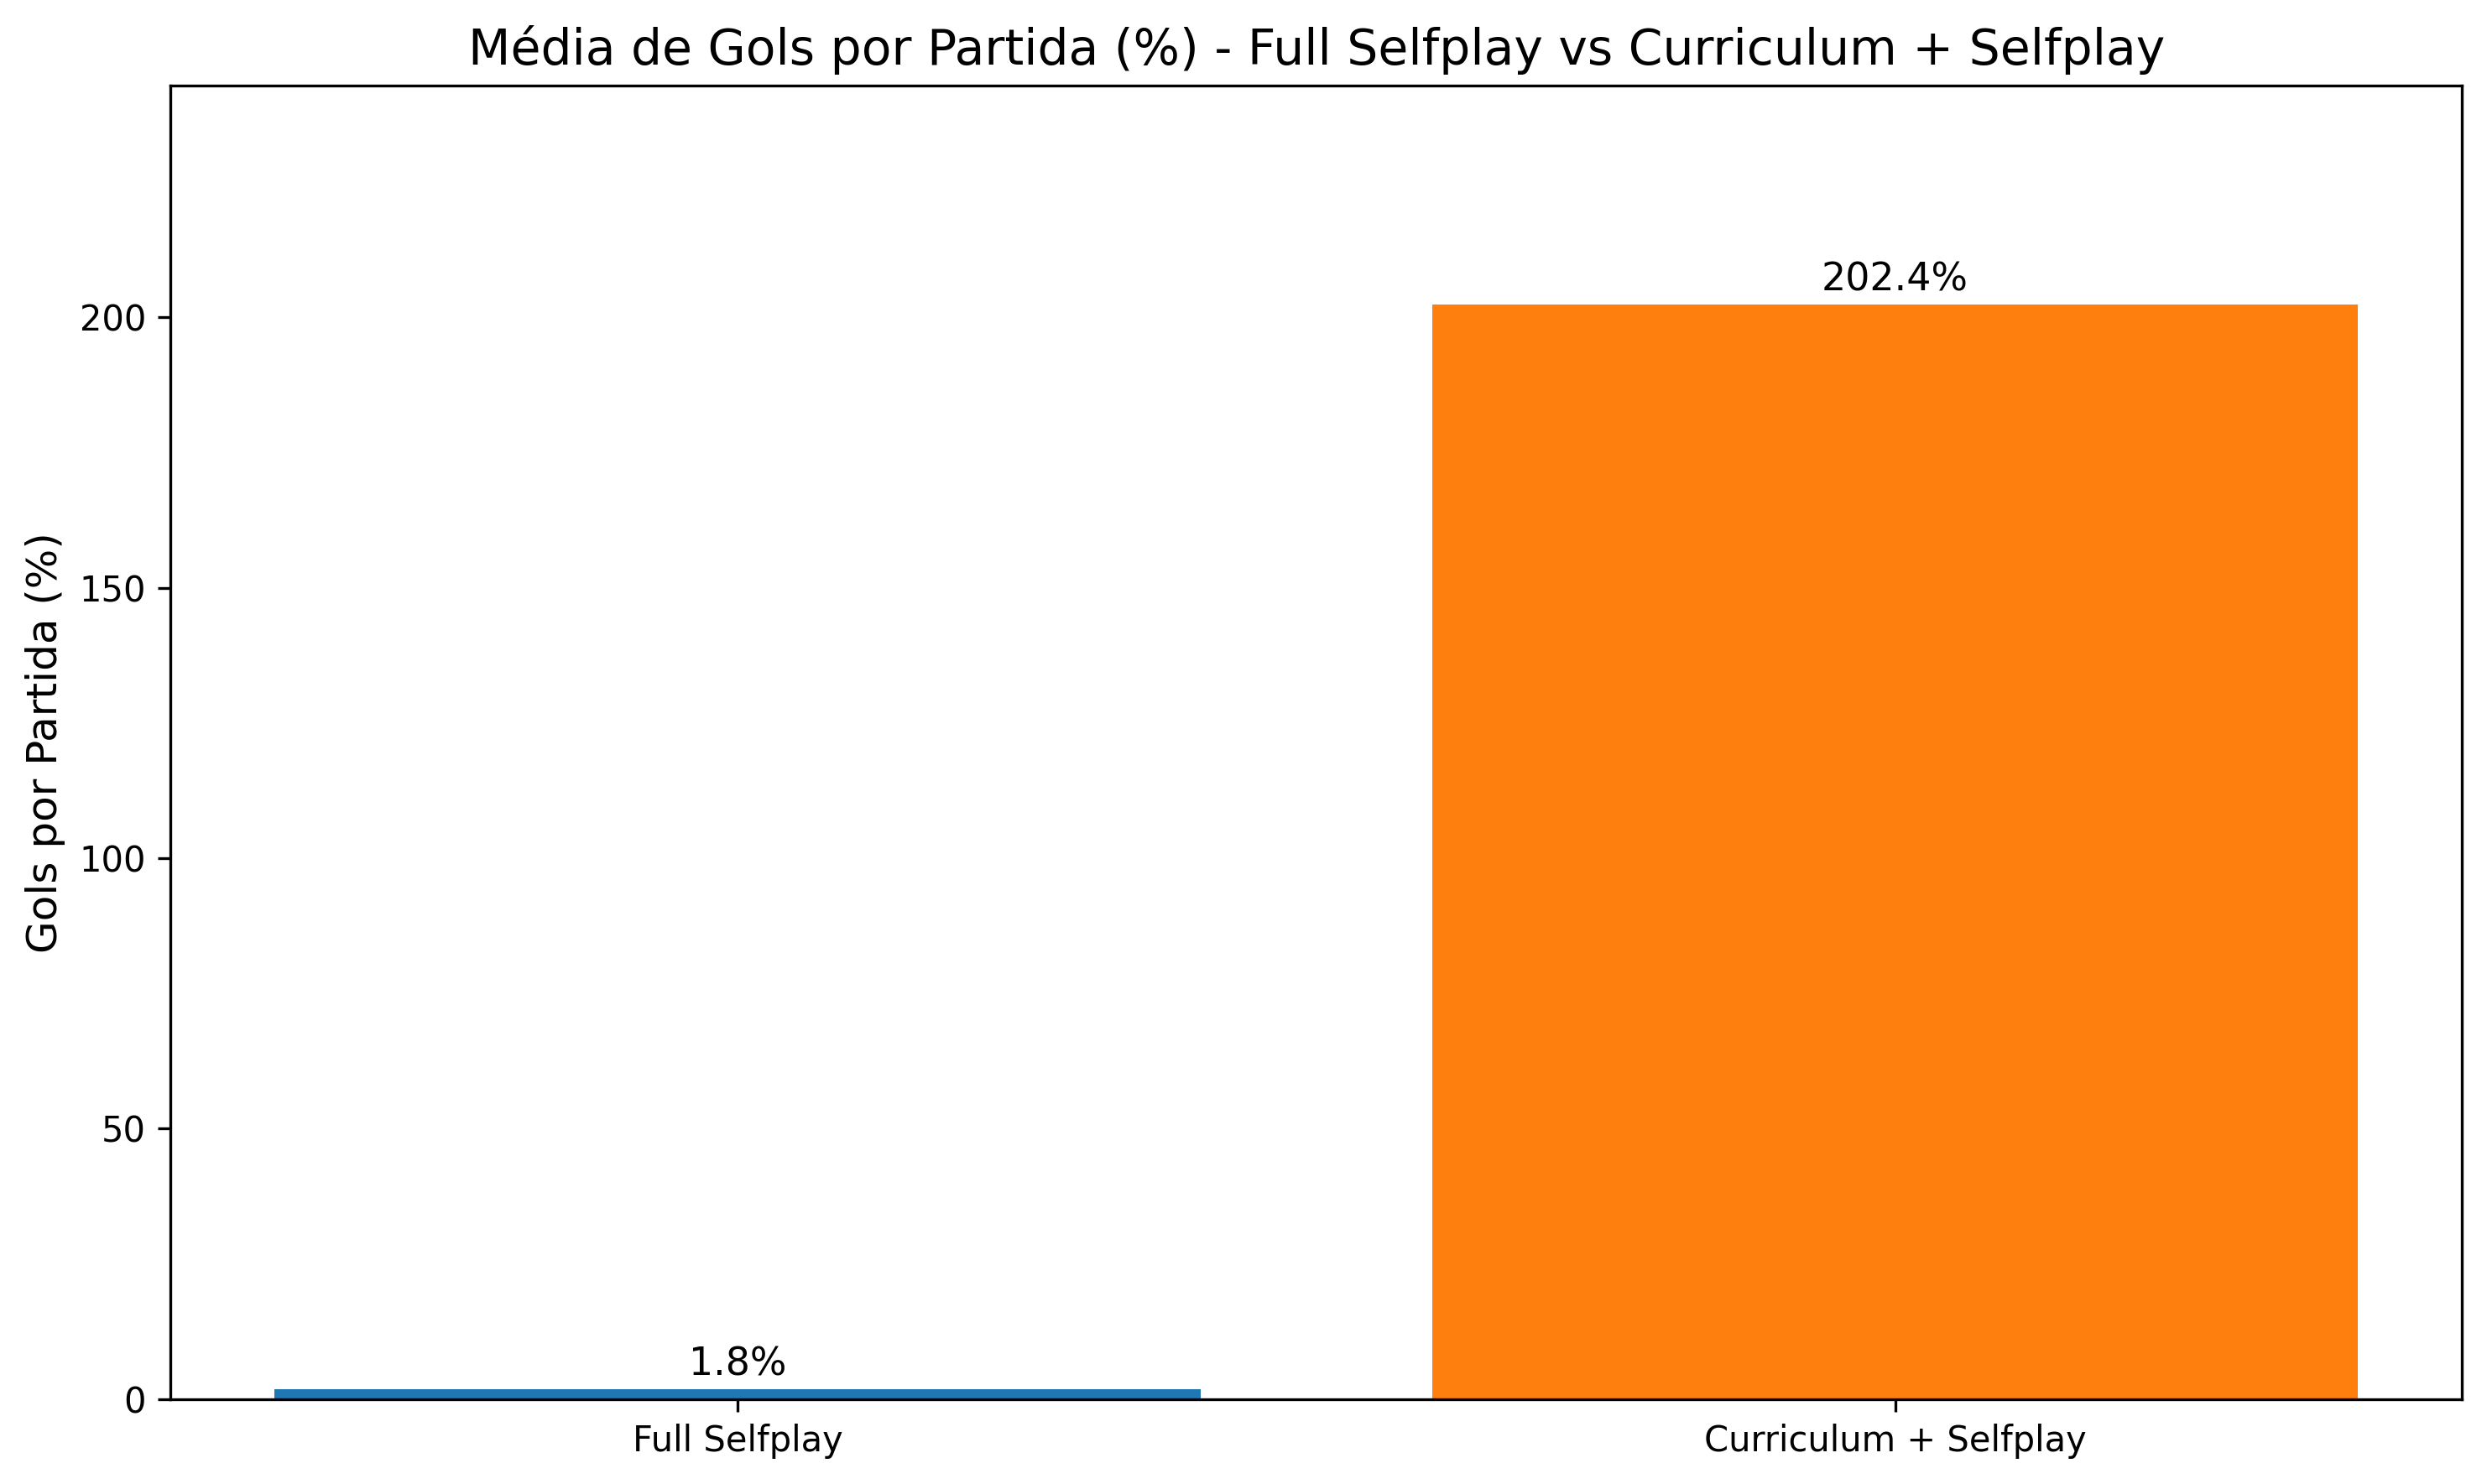
\includegraphics[width=0.8\textwidth]{fig/graficos_trabalho/graficos_torneios/torneios/percentual_gols_full_selfplay_vs_curriculum_+_selfplay.png}
    \caption{Percentual de gols no Torneio 2: Full Selfplay vs Curriculum + Selfplay}
    \label{fig:percentual_gols_torneio2}
\end{figure}

As Figuras \ref{fig:percentual_gols_torneio1} e \ref{fig:percentual_gols_torneio2} ilustram a distribuição percentual dos gols marcados em cada torneio, evidenciando a magnitude da transformação no desempenho ofensivo. No Torneio 1, o Full Selfplay foi responsável por 89,7\% dos gols marcados, enquanto no Torneio 2, o Curriculum + Selfplay marcou impressionantes 99,1\% dos gols.

Esta disparidade extrema na capacidade ofensiva pode ser atribuída ao efeito sinérgico da abordagem combinada. O curriculum learning proporciona uma base sólida de habilidades fundamentais que, quando refinadas através do self-play, resultam em estratégias ofensivas excepcionalmente eficazes. O contraste entre o desempenho do Full Selfplay nos dois torneios sugere que o modelo combinado não apenas desenvolve políticas superiores, mas também consegue neutralizar efetivamente as estratégias do Full Selfplay, limitando drasticamente sua capacidade ofensiva.

\subsection{Análise de Trade-offs entre Abordagens}

Uma observação importante que emerge da análise dos dados dos torneios é o claro trade-off entre as diferentes abordagens de treinamento. A Tabela \ref{tab:comparacao_abordagens_detalhada} resume as principais métricas para cada abordagem nos confrontos diretos, facilitando a visualização destes trade-offs.

\begin{table}[H]
    \centering
    \begin{tabular}{|c|c|c|c|}
        \hline
        \textbf{Métrica} & \textbf{Curriculum} & \textbf{Full Self-play} & \textbf{Curriculum + Self-play} \\
        \hline
        Vitórias vs Full Self-play & 33 (6,6\%) & - & 430 (86\%) \\
        \hline
        Empates vs Full Self-play & 220 (44\%) & - & 63 (12,6\%) \\
        \hline
        Derrotas vs Full Self-play & 247 (49,4\%) & - & 7 (1,4\%) \\
        \hline
        Gols marcados vs Full Self-play & 58 & - & 1.012 \\
        \hline
        Gols sofridos vs Full Self-play & 503 & - & 9 \\
        \hline
        Média de gols/partida & 0,116 & 0,512* & 2,024 \\
        \hline
        \multicolumn{4}{|l|}{* Média calculada considerando os dois torneios (512 gols em 1000 partidas)} \\
        \hline
    \end{tabular}
    \caption{Comparação detalhada entre as três abordagens de treinamento nos torneios}
    \label{tab:comparacao_abordagens_detalhada}
\end{table}

A análise desta tabela revela padrões claros que caracterizam cada abordagem:

\begin{enumerate}
    \item \textbf{Curriculum Learning puro}: Desenvolve agentes com capacidades defensivas significativas, evidenciadas pelo alto número de empates (44\%) mesmo contra o Full Self-play. No entanto, apresenta limitações severas na capacidade ofensiva, com apenas 0,116 gols por partida e baixa taxa de vitórias (6,6\%). Sua estratégia parece focada na neutralização do adversário, mas com dificuldades para criar situações ofensivas efetivas.
    
    \item \textbf{Full Self-play}: Produz agentes com capacidades ofensivas e defensivas moderadamente equilibradas, conseguindo dominar o Curriculum puro (49,4\% de vitórias), mas sendo completamente superado pela abordagem combinada (apenas 1,4\% de vitórias). Esta abordagem baseia-se na exploração auto-dirigida do espaço de estados, resultando em políticas funcionais, mas subótimas.
    
    \item \textbf{Curriculum + Self-play}: Representa uma síntese poderosa que maximiza os benefícios de ambas as abordagens anteriores. Demonstra capacidade ofensiva extraordinária (2,024 gols por partida) combinada com defesa quase impenetrável (apenas 9 gols sofridos em 500 partidas). O resultado é uma dominância esmagadora sobre o Full Self-play, com 86\% de vitórias e mais de 100 vezes mais gols marcados.
\end{enumerate}

Estes resultados confirmam a hipótese central deste trabalho: o curriculum learning proporciona fundamentos sólidos que, quando refinados através do self-play competitivo, resultam em políticas significativamente superiores às desenvolvidas por qualquer uma das abordagens isoladamente.

A análise dos torneios revela aspectos particularmente interessantes sobre a transferência de conhecimento entre fases de treinamento. O modelo Curriculum puro, embora limitado ofensivamente, demonstra capacidades defensivas substanciais, como evidenciado pelo alto número de empates contra o Full Self-play. Quando estas capacidades defensivas são combinadas com o refinamento tático proporcionado pelo self-play, o resultado é um agente com defesa sólida e ataque extremamente eficaz.

Um aspecto notável é a diferença no desempenho do Full Self-play entre os dois torneios. Contra o Curriculum puro, ele demonstra dominância clara, mas contra o Curriculum + Self-play, seu desempenho colapsa. Isto sugere que a abordagem combinada não apenas desenvolve políticas eficazes, mas também consegue neutralizar estrategicamente as políticas aprendidas pelo Full Self-play, explorando suas vulnerabilidades de forma sistemática.

Em síntese, a abordagem combinada Curriculum + Self-play demonstra o melhor equilíbrio entre capacidades ofensivas e defensivas, com uma superioridade que transcende a simples soma das vantagens individuais de cada método. Este efeito sinérgico valida a importância do desenvolvimento estruturado de habilidades fundamentais antes da exposição a cenários competitivos complexos, estabelecendo um paradigma promissor para o treinamento de agentes em ambientes multiagente como o futebol de robôs.

\section{Análise das Métricas de Aprendizado por Reforço}
\label{sec:analise_metricas_aprendizado}

Além das métricas específicas do domínio do futebol de robôs, uma análise detalhada das métricas básicas de aprendizado por reforço fornece insights valiosos sobre os processos internos dos algoritmos durante o treinamento. Esta seção explora três métricas fundamentais: entropia da política, perda da política e variância explicada da função valor, comparando o comportamento dessas métricas entre as abordagens Selfplay após Curriculum e Full Selfplay.

\subsection{Entropia da Política}

A entropia da política é uma métrica que quantifica o grau de aleatoriedade ou exploração nas decisões do agente. Valores mais altos (menos negativos) indicam maior exploração, enquanto valores mais baixos (mais negativos) sugerem maior certeza nas ações escolhidas. A Figura \ref{fig:policy_entropy} apresenta a comparação da entropia da política entre as duas abordagens ao longo do treinamento.

\begin{figure}[H]
    \centering
    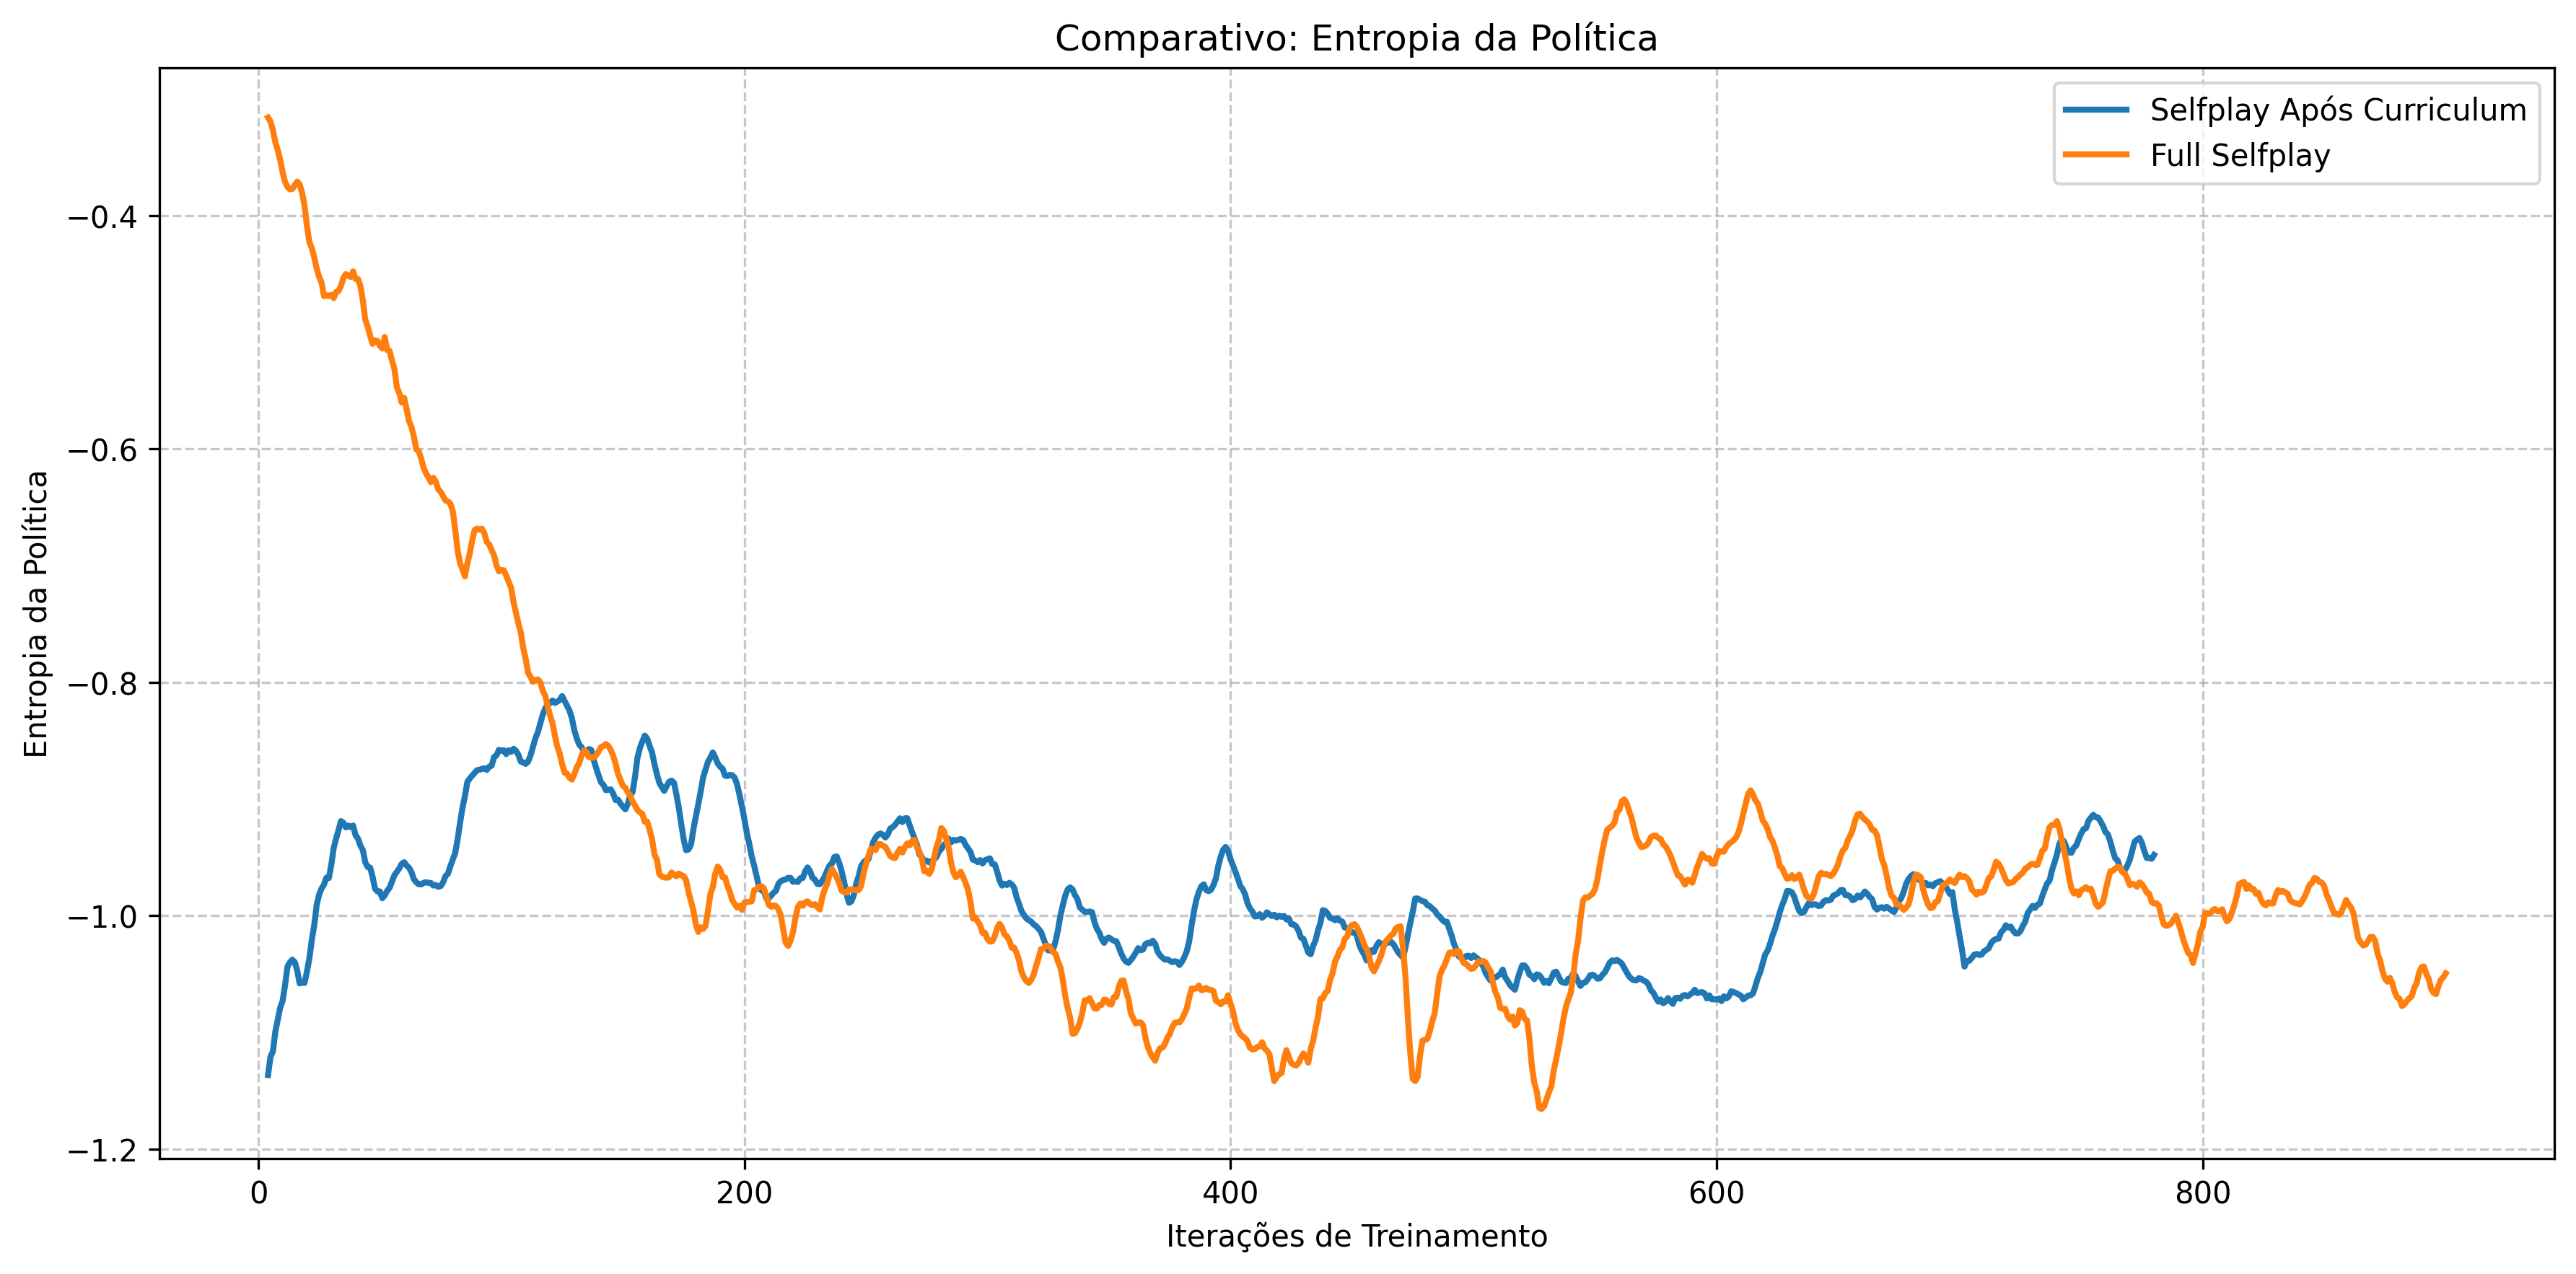
\includegraphics[width=0.95\textwidth]{fig/graficos_trabalho/graficos_experimentos/geral/comparativo_entropia_politica.png}
    \caption{Comparativo da entropia da política com iterações alinhadas entre as abordagens Selfplay após Curriculum e Full Selfplay}
    \label{fig:policy_entropy}
\end{figure}

A análise do gráfico revela diferenças significativas nos padrões de exploração-explotação entre as duas abordagens. O Full Selfplay (linha laranja) inicia o treinamento com valores de entropia mais altos (próximos a -0,3), indicando uma política mais exploratória, o que é esperado para agentes que começam o aprendizado sem conhecimento prévio. Em contraste, o Selfplay após Curriculum (linha azul) começa com valores de entropia significativamente mais baixos (aproximadamente -1,1), sugerindo uma política já mais determinística.

Esta diferença inicial é particularmente reveladora: agentes treinados com curriculum learning iniciam a fase de selfplay com políticas mais refinadas e menos aleatórias, evidenciando que o conhecimento adquirido durante os estágios do curriculum proporciona maior certeza nas ações a serem tomadas.

Após aproximadamente 150-200 iterações, observa-se uma convergência nas entropias, com ambas as abordagens chegando a valores similares. No entanto, é notável que o Full Selfplay apresenta maior volatilidade ao longo de todo o treinamento, com oscilações mais pronunciadas, enquanto o Selfplay após Curriculum mantém níveis mais estáveis de entropia, sugerindo um processo de aprendizado mais consistente e menos errático.

\subsection{Perda da Política}

A perda da política é uma métrica que reflete a divergência entre a política atual e a política que seria ótima segundo as estimativas atuais da função de valor. Em algoritmos como PPO, a minimização desta perda é um dos objetivos principais do processo de otimização. A Figura \ref{fig:policy_loss} apresenta a evolução desta métrica durante o treinamento.

\begin{figure}[H]
    \centering
    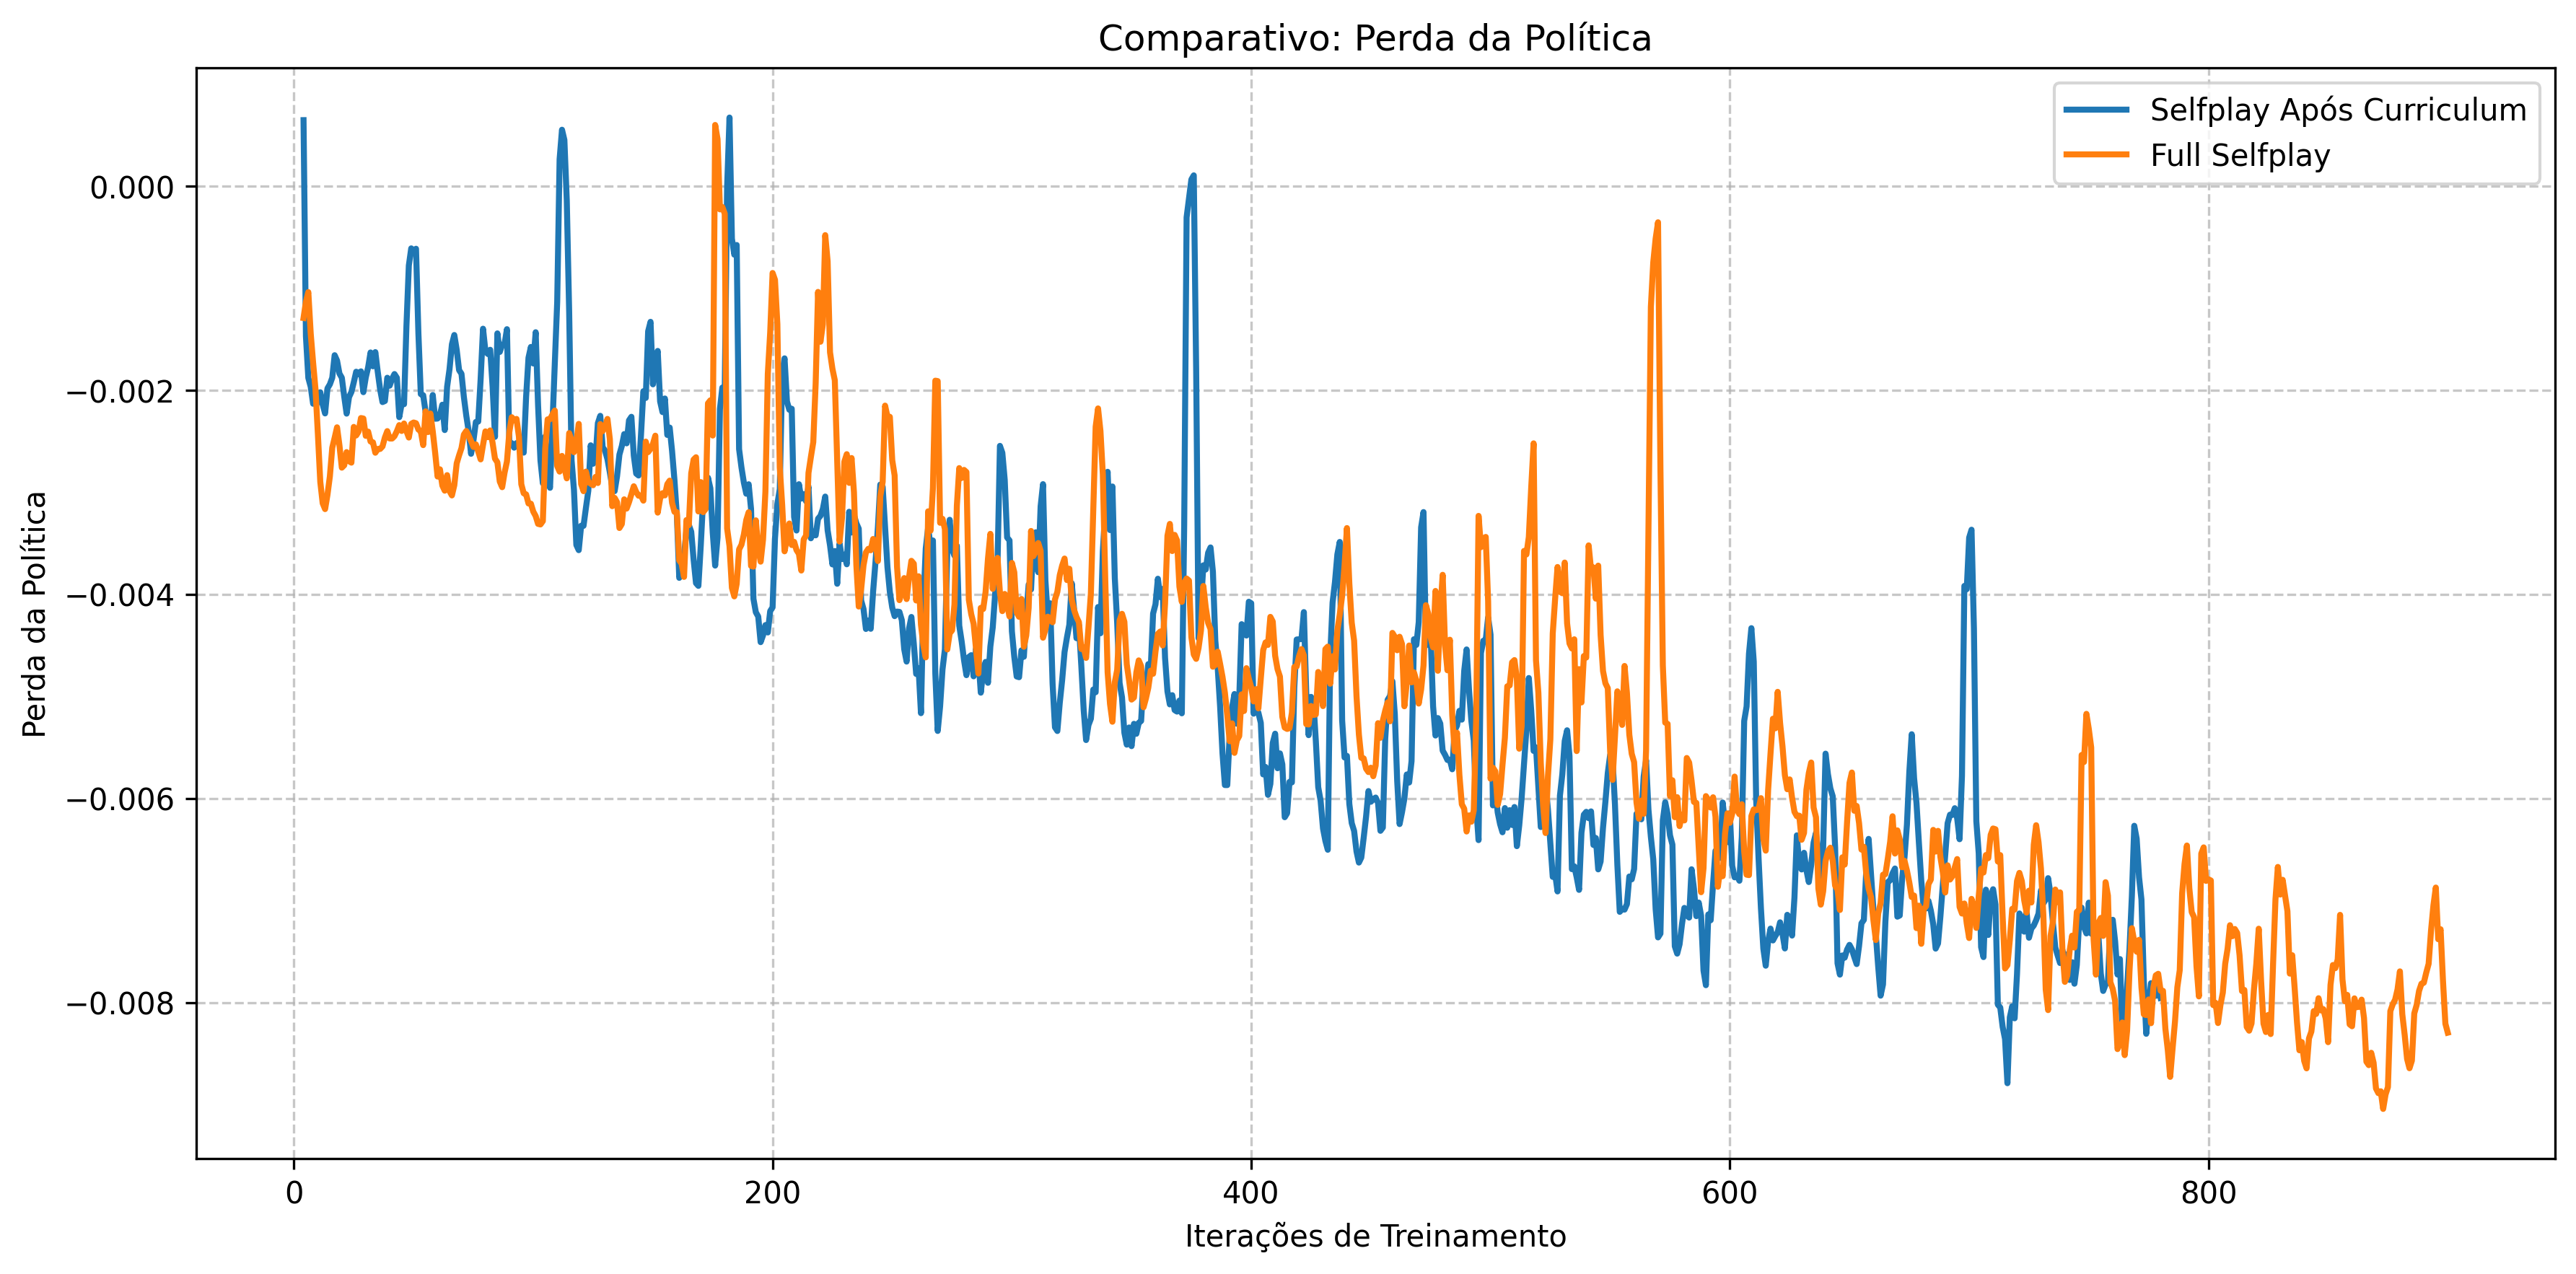
\includegraphics[width=0.95\textwidth]{fig/graficos_trabalho/graficos_experimentos/geral/comparativo_perda_politica.png}
    \caption{Comparativo da perda da política com iterações alinhadas entre as abordagens Selfplay após Curriculum e Full Selfplay}
    \label{fig:policy_loss}
\end{figure}

O gráfico de perda da política mostra um comportamento interessante: ambas as abordagens iniciam com valores similares e seguem uma tendência geral de redução da perda ao longo do treinamento, o que indica uma melhoria progressiva nas políticas. No entanto, há diferenças notáveis na trajetória dessa redução.

Observa-se que ambas as abordagens apresentam alta volatilidade, com várias oscilações ao longo do processo. Esta característica é típica de ambientes competitivos como o self-play, onde as mudanças na política de um oponente podem temporariamente aumentar a perda até que o agente se adapte.

Um aspecto particularmente relevante é que o Full Selfplay continua seu treinamento por mais iterações e alcança valores de perda mais negativos nas fases finais. Isto pode indicar que, sem o benefício do curriculum inicial, esta abordagem requer um período mais longo de refinamento para atingir níveis comparáveis de otimização da política.

A análise conjunta com as outras métricas sugere que, embora o Full Selfplay eventualmente alcance valores de perda similares ou até melhores, o caminho para chegar a este ponto é mais longo e menos eficiente comparado ao Selfplay após Curriculum.

\subsection{Variância Explicada da Função Valor}

A variância explicada é uma métrica que avalia a qualidade da função valor aprendida pelo agente, indicando quão bem o modelo consegue prever retornos futuros. Valores próximos a 1 indicam alta precisão nas previsões, enquanto valores mais baixos sugerem maior incerteza. A Figura \ref{fig:explained_variance} apresenta a comparação desta métrica entre as duas abordagens.

\begin{figure}[H]
    \centering
    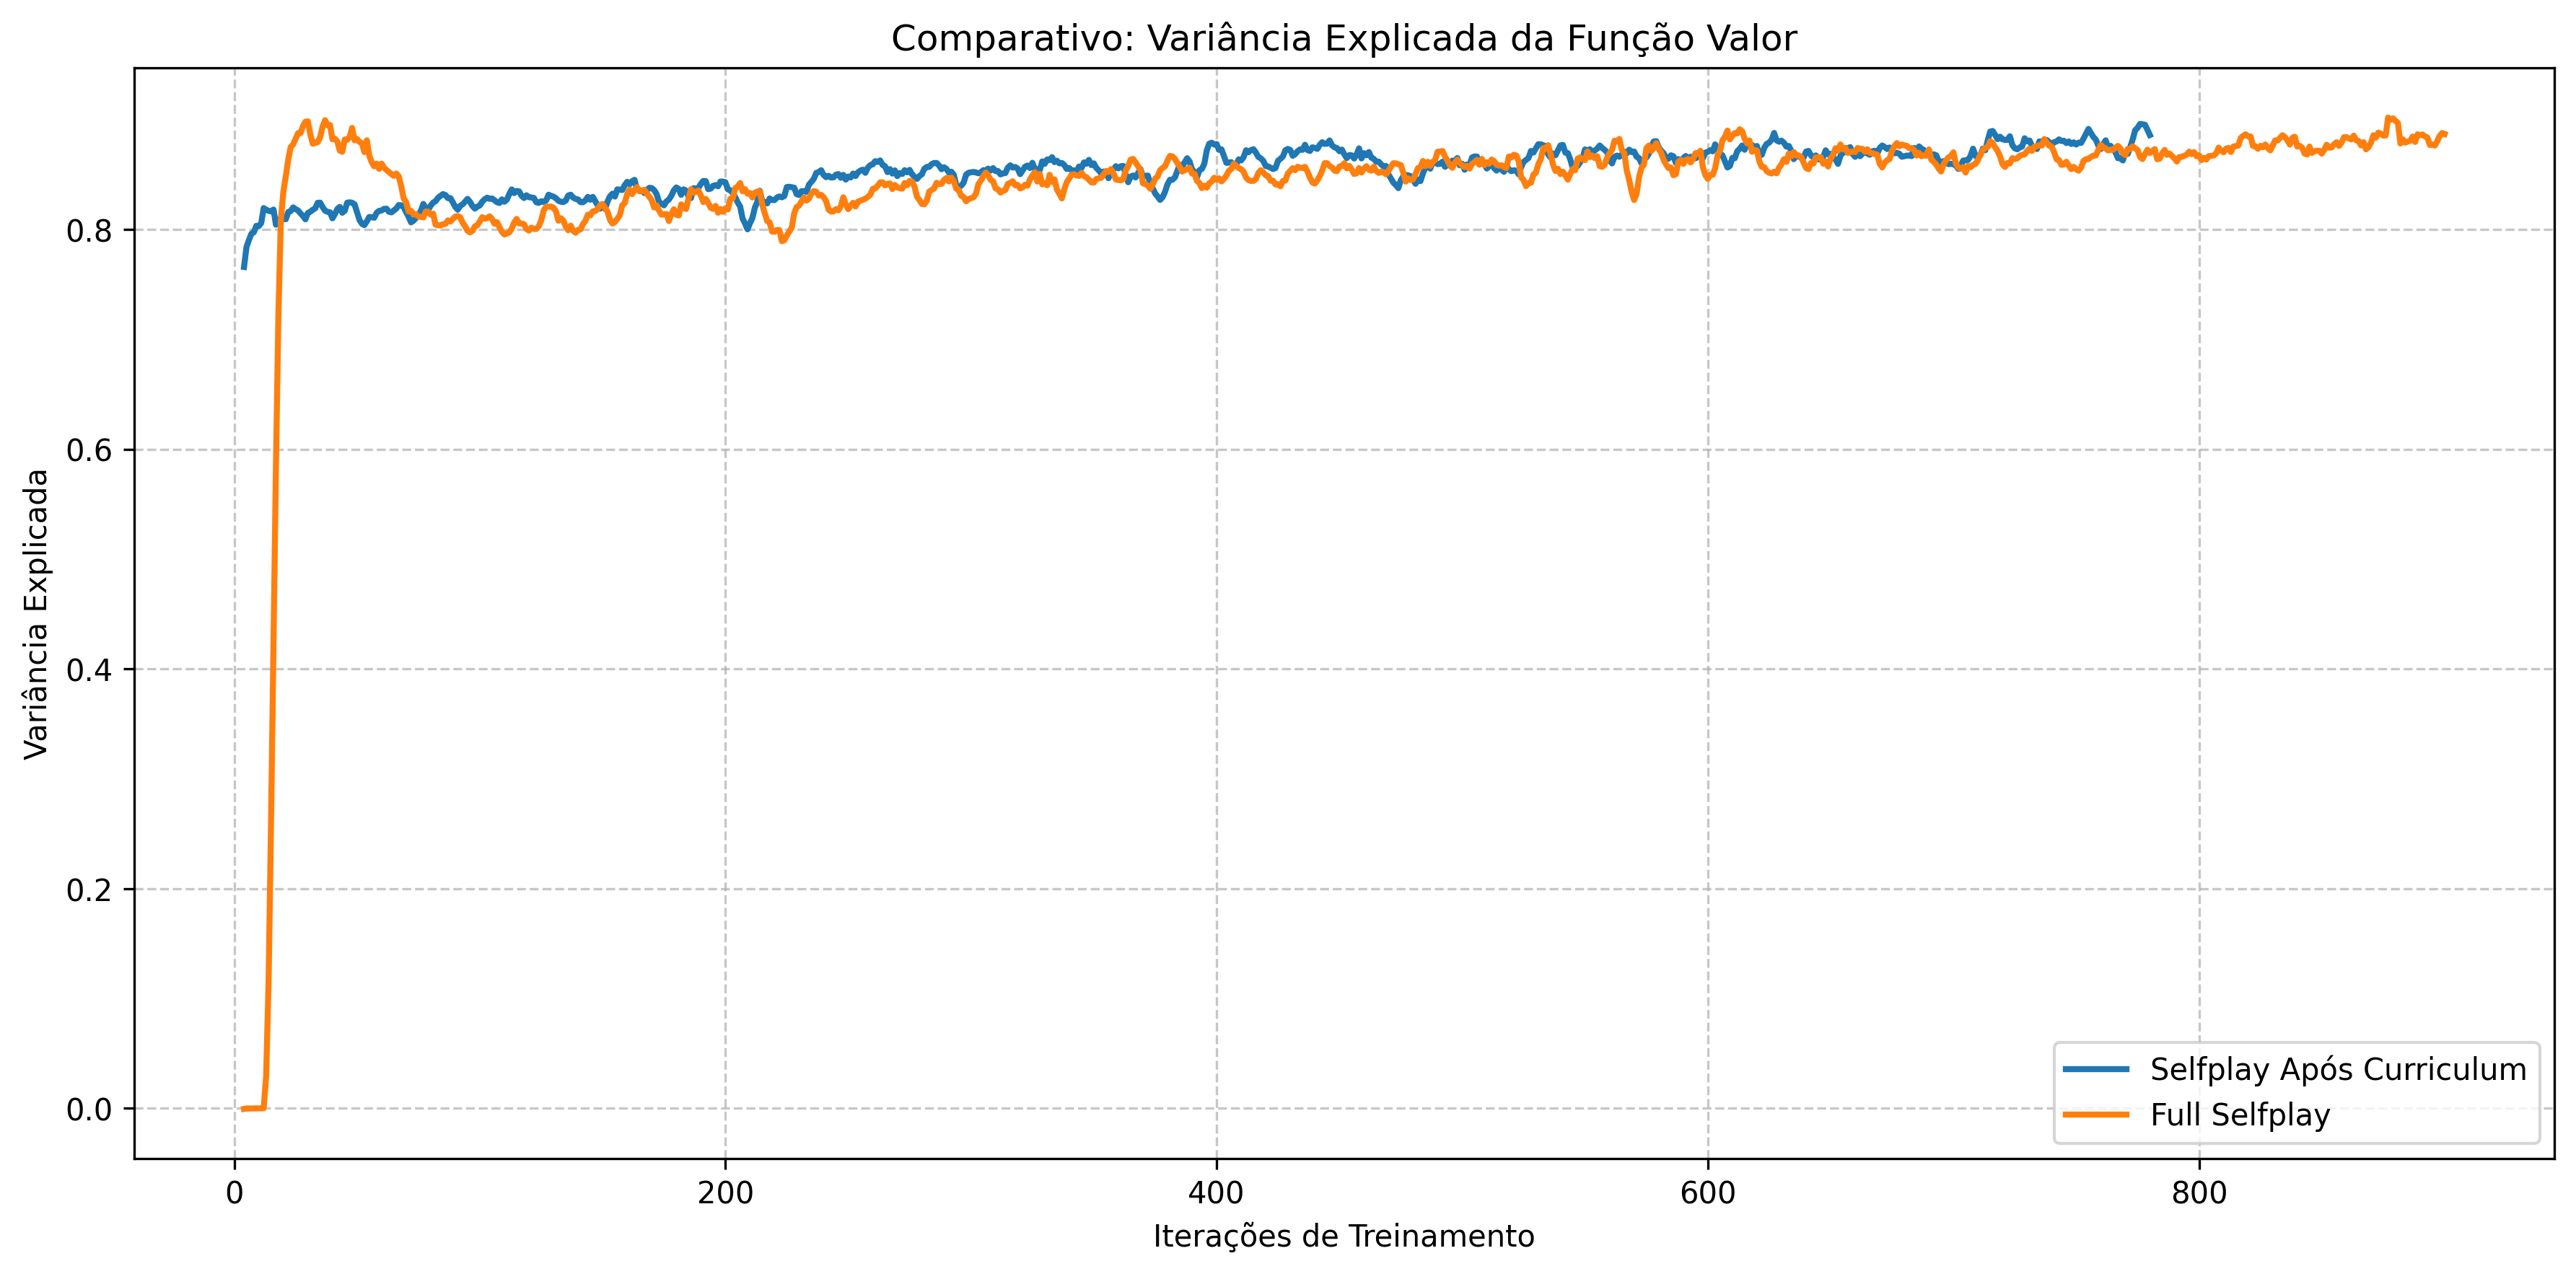
\includegraphics[width=0.95\textwidth]{fig/graficos_trabalho/graficos_experimentos/geral/comparativo_variancia_explicada.png}
    \caption{Comparativo da variância explicada da função valor com iterações alinhadas entre as abordagens Selfplay após Curriculum e Full Selfplay}
    \label{fig:explained_variance}
\end{figure}

A análise do gráfico de variância explicada revela padrões distintos no desenvolvimento da função valor. O Full Selfplay (linha laranja) apresenta um comportamento curioso nas primeiras iterações, com um pico inicial seguido por uma queda abrupta. Este padrão pode ser atribuído a uma superestimação inicial da capacidade preditiva, seguida por um ajuste à medida que o agente enfrenta situações mais diversificadas.

Em contraste, o Selfplay após Curriculum (linha azul) inicia com valores mais estáveis, sem os extremos observados no Full Selfplay. Esta estabilidade inicial é mais uma evidência dos benefícios do treinamento curricular prévio, que proporciona ao agente uma base mais sólida para estimar recompensas futuras.

Após aproximadamente 200 iterações, ambas as abordagens convergem para valores similares de variância explicada, em torno de 0,85, indicando que ambos os métodos eventualmente desenvolvem funções valor de qualidade comparável. No entanto, o caminho para atingir esta convergência é notavelmente diferente, com o Selfplay após Curriculum demonstrando maior consistência ao longo do processo.

Nas fases finais do treinamento, após a convergência, ambas as abordagens mantêm níveis similares e estáveis de variância explicada, sugerindo que, embora o processo de aprendizado seja diferente, o resultado final em termos de capacidade preditiva da função valor é comparável.

\subsection{Implicações para o Processo de Aprendizagem}

A análise integrada das três métricas básicas de aprendizado por reforço revela padrões consistentes que destacam as diferenças fundamentais entre as abordagens Selfplay após Curriculum e Full Selfplay.

Em primeiro lugar, observa-se que o Selfplay após Curriculum consistentemente demonstra maior estabilidade nas fases iniciais e intermediárias do treinamento. Esta característica é particularmente valiosa em cenários complexos como o futebol de robôs, onde a volatilidade excessiva pode levar a políticas subótimas ou comportamentos indesejados.

Em segundo lugar, a transição mais suave nas métricas de aprendizado do Selfplay após Curriculum sugere que o conhecimento adquirido durante os estágios do curriculum proporciona um ponto de partida mais avançado para o desenvolvimento de políticas competitivas. Esta vantagem inicial se traduz em um processo de aprendizado mais eficiente, requerendo menos iterações para atingir níveis comparáveis de desempenho.

Por fim, embora ambas as abordagens eventualmente convirjam para valores similares nas métricas analisadas, o caminho para esta convergência é significativamente diferente. O Selfplay após Curriculum oferece um processo de aprendizado mais direto e consistente, enquanto o Full Selfplay requer um período mais longo de ajustes e adaptações antes de atingir estabilidade.

Estas observações corroboram a hipótese central deste trabalho: o curriculum learning como fase preparatória proporciona um alicerce mais sólido para o desenvolvimento de políticas complexas, resultando em um processo de aprendizado mais eficiente e estável durante o subsequente treinamento competitivo via self-play.

\section{Discussão dos Resultados}
\label{sec:discussao_resultados}

A análise dos resultados experimentais permite estabelecer conclusões substantivas sobre a eficácia da abordagem proposta. Esta seção sintetiza as principais descobertas e suas implicações.

\subsection{Síntese dos Resultados Experimentais}

Os experimentos realizados revelam superioridade consistente da abordagem combinada (Curriculum + Self-play) em relação às alternativas. Esta superioridade manifesta-se em três dimensões principais:

\begin{enumerate}
    \item \textbf{Desempenho competitivo}: A taxa de vitória de 86\% (430 vitórias em 500 partidas) contra o Full Self-play, que obteve apenas 1,4\% (7 vitórias), representa evidência inequívoca da eficácia da abordagem proposta. A capacidade de marcar gols também se destaca, com média de 2,024 gols por partida (1012 gols em 500 partidas), muito superior aos 0,018 gols por partida do Full Self-play (9 gols em 500 partidas).

    \item \textbf{Eficiência computacional}: A redução de aproximadamente 15\% no tempo total de treinamento (7,4 horas versus 8,7 horas) demonstra ganho significativo de eficiência, fator crítico para aplicações práticas.

    \item \textbf{Estabilidade do aprendizado}: As métricas básicas de aprendizado por reforço (entropia da política, perda da política e variância explicada) evidenciam um processo mais estável e consistente, com menor volatilidade durante as fases críticas do treinamento.
\end{enumerate}

Os dados apresentam ainda um padrão claro de complementaridade entre as abordagens. O Curriculum Learning isolado produz agentes com desempenho limitado (apenas 33 vitórias contra 247 do Full Self-play em 500 partidas), enquanto o Self-play puro desenvolve agentes com capacidades mais equilibradas, porém inferiores à abordagem combinada. A estratégia de Curriculum + Self-play potencializa as vantagens de ambas as abordagens, resultando em agentes tecnicamente refinados e taticamente eficazes.

\subsection{Confirmação da Hipótese}

Os resultados obtidos confirmam consistentemente a hipótese central deste trabalho: o curriculum learning como fase preparatória para o self-play melhora significativamente as políticas aprendidas, resultando em agentes com desempenho superior.

Esta confirmação apoia-se em evidências estatisticamente significativas observadas em múltiplos cenários de avaliação e métricas diversas. O curriculum learning proporciona fundamentos técnicos que permitem ao agente aproveitar melhor a fase competitiva do self-play, acelerando e otimizando o desenvolvimento de políticas eficazes.

\subsection{Limitações do Estudo}

Apesar dos resultados promissores, algumas limitações devem ser consideradas:

\begin{itemize}
    \item \textbf{Generalização para ambientes físicos}: Os experimentos foram conduzidos exclusivamente em simulação, existindo o desafio conhecido do reality gap na transferência para robôs reais.
    
    \item \textbf{Sensibilidade paramétrica}: A eficácia do curriculum learning depende do design apropriado das tarefas e critérios de promoção, cuja otimização sistemática não foi completamente explorada.
    
    \item \textbf{Especificidade do domínio}: Embora os princípios sejam potencialmente generalizáveis, os resultados foram validados especificamente no contexto do futebol de robôs.
\end{itemize}

\subsection{Implicações para Aprendizado por Reforço}

As descobertas deste trabalho têm implicações que transcendem o domínio específico do futebol de robôs:

\begin{enumerate}
    \item \textbf{Valor do aprendizado estruturado}: Em domínios complexos com espaço de ações amplo e feedback esparso, o treinamento progressivo demonstra benefícios significativos.
    
    \item \textbf{Importância de métricas diversificadas}: A análise exclusiva de métricas convencionais (como recompensa acumulada) pode obscurecer nuances importantes no processo de aprendizado e qualidade das políticas.
    
    \item \textbf{Complementaridade de abordagens}: Diferentes técnicas de treinamento podem desenvolver habilidades complementares, cuja combinação resulta em agentes com desempenho superior à soma das partes.
\end{enumerate}

A metodologia desenvolvida neste trabalho oferece um framework transferível para o design de trajetórias de aprendizado em ambientes multiagentes complexos, especialmente aqueles que compartilham características como necessidade de coordenação, feedback esparso e complexidade estratégica.

\section{Considerações sobre os Estágios do Curriculum}
\label{sec:analise_estagios}

Esta seção analisa sucintamente o desempenho dos agentes em cada estágio do curriculum e sua transição para the self-play, complementando os resultados já apresentados.

\subsection{Progresso no Curriculum Task 0}

No Curriculum Task 0, os agentes atingiram o critério de promoção (80\% de sucesso em 100 episódios) após aproximadamente 0,35 horas (21 minutos) de treinamento, utilizando menos da metade do orçamento temporal alocado. Essa eficiência indica que o design da tarefa proporcionou um desafio apropriado para o desenvolvimento das habilidades básicas de controle e movimentação, que serviram como fundamento para estágios posteriores.

\subsection{Progresso no Curriculum Task 1}

No Curriculum Task 1, focado em habilidades ofensivas, os agentes completaram o estágio em aproximadamente 0,35 horas (21 minutos) de treinamento. Neste estágio, observou-se o desenvolvimento de estratégias coordenadas, incluindo posicionamento tático e padrões de passe. A transição eficiente entre os estágios validou o design progressivo das tarefas, confirmando a eficácia da sequência de aprendizado.

\subsection{Transição para Self-Play}

A transição para o self-play demonstrou a vantagem da preparação via curriculum. Os agentes com treinamento prévio apresentaram adaptação mais rápida ao ambiente competitivo, evidenciada pelo crescimento superior da recompensa nas primeiras horas do self-play e menor volatilidade nas métricas de desempenho. Esta transição mais suave corrobora os resultados apresentados nas seções anteriores, onde a estabilidade do aprendizado foi identificada como uma das principais vantagens da abordagem combinada.

A análise dos estágios do curriculum permite compreender a origem das vantagens observadas na abordagem Selfplay após Curriculum, especialmente a maior eficiência computacional (redução de 15\% no tempo total) e estabilidade nas métricas de aprendizado por reforço discutidas anteriormente.

\section{Conclusões Experimentais}
\label{sec:conclusoes_experimentais}

Os experimentos realizados neste trabalho permitem extrair conclusões importantes sobre a eficácia da abordagem proposta e suas implicações para o treinamento de agentes em ambientes complexos e multiagentes.

\subsection{Principais Descobertas}

A análise integrada dos resultados experimentais permite identificar as seguintes descobertas principais:

\begin{enumerate}
    \item \textbf{Eficácia do curriculum learning}: A abordagem proposta, combinando curriculum learning e self-play, demonstrou superioridade estatisticamente significativa em termos de desempenho global, evidenciada pela maior taxa de vitória em confrontos diretos (86\% de vitórias contra 1,4\% do Full Self-play) e melhor equilíbrio entre métricas ofensivas e defensivas.
    
    \item \textbf{Desenvolvimento de habilidades fundamentais}: O curriculum learning promoveu o desenvolvimento eficiente de habilidades fundamentais em apenas 42 minutos de treinamento, resultando em melhorias significativas nas métricas de continuidade do jogo e controle técnico.
    
    \item \textbf{Aprendizado mais estável}: A abordagem proposta apresentou maior estabilidade durante o processo de aprendizagem, com menor variabilidade nas métricas de desempenho e progressão mais consistente, reduzindo o tempo total de treinamento em 15\% (7,4 horas vs 8,7 horas do Full Self-play).
    
    \item \textbf{Trade-off entre agressividade e controle}: O modelo treinado com curriculum learning desenvolveu um estilo de jogo mais equilibrado, priorizando controle técnico e manutenção da posse de bola sobre tentativas arriscadas de finalização, resultando em uma média superior de gols por partida (2,02 vs 0,018 do Full Self-play).
\end{enumerate}

Estas descobertas corroboram a premissa central deste trabalho: que o aprendizado estruturado e progressivo proporcionado pelo curriculum learning oferece vantagens significativas para o treinamento de agentes em ambientes complexos como o futebol de robôs.

\subsection{Implicações para Aprendizado por Reforço em Ambientes Multiagentes}

Os resultados obtidos têm implicações mais amplas para o campo do aprendizado por reforço em ambientes multiagentes, estendendo-se além do domínio específico do futebol de robôs.

Em primeiro lugar, os experimentos demonstram o valor do treinamento progressivo em cenários onde o espaço de ações é amplo e o feedback é esparso. O curriculum learning oferece uma abordagem estruturada para decompor problemas complexos em desafios gerenciáveis, facilitando o desenvolvimento de competências em uma sequência lógica.

Em segundo lugar, os resultados destacam a importância de considerar métricas diversificadas na avaliação do desempenho dos agentes. A análise restrita a métricas convencionais (como recompensa acumulada) pode não capturar nuances importantes no comportamento e na qualidade das políticas aprendidas.

Por fim, o equilíbrio superior entre características ofensivas e defensivas observado no modelo proposto sugere que o curriculum learning pode promover o desenvolvimento de políticas mais robustas e versáteis, capazes de adaptar-se a diferentes contextos e adversários.

\subsection{Transferibilidade dos Resultados}

Uma consideração importante é a transferibilidade dos resultados obtidos para outros domínios e aplicações. Embora os experimentos tenham sido realizados no contexto específico do futebol de robôs, os princípios fundamentais da abordagem proposta podem ser adaptados para diversos cenários multiagentes.

O framework de curriculum learning desenvolvido neste trabalho oferece uma metodologia generalizável para o design de trajetórias de aprendizado em ambientes complexos. Os critérios de promoção adaptativos e a integração com self-play representam contribuições que podem ser aplicadas em domínios que compartilham características como:

\begin{itemize}
    \item Espaço de ações amplo e contínuo
    \item Necessidade de coordenação multiagente
    \item Feedback esparso ou atrasado
    \item Complexidade estratégica e tática
    \item Oposição adaptativa
\end{itemize}

Exemplos potenciais de aplicação incluem robótica colaborativa, sistemas de transporte autônomos coordenados, gerenciamento de recursos distribuídos e simulações militares.

A metodologia experimental desenvolvida, incluindo as métricas de avaliação e o sistema de torneios, também oferece um template valioso para a avaliação comparativa de diferentes abordagens de treinamento em ambientes complexos. 